\documentclass[twoside]{book}

% Packages required by doxygen
\usepackage{calc}
\usepackage{doxygen}
\usepackage{graphicx}
\usepackage[utf8]{inputenc}
\usepackage{makeidx}
\usepackage{multicol}
\usepackage{multirow}
\usepackage{fixltx2e}
\PassOptionsToPackage{warn}{textcomp}
\usepackage{textcomp}
\usepackage[nointegrals]{wasysym}
\usepackage[table]{xcolor}

% Font selection
\usepackage[T1]{fontenc}
\usepackage{mathptmx}
\usepackage[scaled=.90]{helvet}
\usepackage{courier}
\usepackage{amssymb}
\usepackage{sectsty}
\renewcommand{\familydefault}{\sfdefault}
\allsectionsfont{%
  \fontseries{bc}\selectfont%
  \color{darkgray}%
}
\renewcommand{\DoxyLabelFont}{%
  \fontseries{bc}\selectfont%
  \color{darkgray}%
}
\newcommand{\+}{\discretionary{\mbox{\scriptsize$\hookleftarrow$}}{}{}}

% Page & text layout
\usepackage{geometry}
\geometry{%
  a4paper,%
  top=2.5cm,%
  bottom=2.5cm,%
  left=2.5cm,%
  right=2.5cm%
}
\tolerance=750
\hfuzz=15pt
\hbadness=750
\setlength{\emergencystretch}{15pt}
\setlength{\parindent}{0cm}
\setlength{\parskip}{0.2cm}
\makeatletter
\renewcommand{\paragraph}{%
  \@startsection{paragraph}{4}{0ex}{-1.0ex}{1.0ex}{%
    \normalfont\normalsize\bfseries\SS@parafont%
  }%
}
\renewcommand{\subparagraph}{%
  \@startsection{subparagraph}{5}{0ex}{-1.0ex}{1.0ex}{%
    \normalfont\normalsize\bfseries\SS@subparafont%
  }%
}
\makeatother

% Headers & footers
\usepackage{fancyhdr}
\pagestyle{fancyplain}
\fancyhead[LE]{\fancyplain{}{\bfseries\thepage}}
\fancyhead[CE]{\fancyplain{}{}}
\fancyhead[RE]{\fancyplain{}{\bfseries\leftmark}}
\fancyhead[LO]{\fancyplain{}{\bfseries\rightmark}}
\fancyhead[CO]{\fancyplain{}{}}
\fancyhead[RO]{\fancyplain{}{\bfseries\thepage}}
\fancyfoot[LE]{\fancyplain{}{}}
\fancyfoot[CE]{\fancyplain{}{}}
\fancyfoot[RE]{\fancyplain{}{\bfseries\scriptsize Generated on Sat Oct 4 2014 14\+:31\+:39 for Battle Tanks by Doxygen }}
\fancyfoot[LO]{\fancyplain{}{\bfseries\scriptsize Generated on Sat Oct 4 2014 14\+:31\+:39 for Battle Tanks by Doxygen }}
\fancyfoot[CO]{\fancyplain{}{}}
\fancyfoot[RO]{\fancyplain{}{}}
\renewcommand{\footrulewidth}{0.4pt}
\renewcommand{\chaptermark}[1]{%
  \markboth{#1}{}%
}
\renewcommand{\sectionmark}[1]{%
  \markright{\thesection\ #1}%
}

% Indices & bibliography
\usepackage{natbib}
\usepackage[titles]{tocloft}
\setcounter{tocdepth}{3}
\setcounter{secnumdepth}{5}
\makeindex

% Hyperlinks (required, but should be loaded last)
\usepackage{ifpdf}
\ifpdf
  \usepackage[pdftex,pagebackref=true]{hyperref}
\else
  \usepackage[ps2pdf,pagebackref=true]{hyperref}
\fi
\hypersetup{%
  colorlinks=true,%
  linkcolor=blue,%
  citecolor=blue,%
  unicode%
}

% Custom commands
\newcommand{\clearemptydoublepage}{%
  \newpage{\pagestyle{empty}\cleardoublepage}%
}


%===== C O N T E N T S =====

\begin{document}

% Titlepage & ToC
\hypersetup{pageanchor=false,
             bookmarks=true,
             bookmarksnumbered=true,
             pdfencoding=unicode
            }
\pagenumbering{roman}
\begin{titlepage}
\vspace*{7cm}
\begin{center}%
{\Large Battle Tanks \\[1ex]\large 1.\+3 }\\
\vspace*{1cm}
{\large Generated by Doxygen 1.8.7}\\
\vspace*{0.5cm}
{\small Sat Oct 4 2014 14:31:39}\\
\end{center}
\end{titlepage}
\clearemptydoublepage
\tableofcontents
\clearemptydoublepage
\pagenumbering{arabic}
\hypersetup{pageanchor=true}

%--- Begin generated contents ---
\chapter{Hierarchical Index}
\section{Class Hierarchy}
This inheritance list is sorted roughly, but not completely, alphabetically\+:\begin{DoxyCompactList}
\item \contentsline{section}{Action\+Data}{\pageref{class_action_data}}{}
\begin{DoxyCompactList}
\item \contentsline{section}{Game\+Management\+Data}{\pageref{class_game_management_data}}{}
\end{DoxyCompactList}
\item \contentsline{section}{actions\+\_\+info}{\pageref{structactions__info}}{}
\item \contentsline{section}{Collision\+Helper}{\pageref{class_collision_helper}}{}
\item \contentsline{section}{coordinate}{\pageref{structcoordinate}}{}
\item \contentsline{section}{Deletable}{\pageref{class_deletable}}{}
\begin{DoxyCompactList}
\item \contentsline{section}{Collidable}{\pageref{class_collidable}}{}
\begin{DoxyCompactList}
\item \contentsline{section}{Barrier}{\pageref{class_barrier}}{}
\item \contentsline{section}{Mine}{\pageref{class_mine}}{}
\item \contentsline{section}{Missile}{\pageref{class_missile}}{}
\item \contentsline{section}{Tank}{\pageref{class_tank}}{}
\item \contentsline{section}{Turret}{\pageref{class_turret}}{}
\end{DoxyCompactList}
\item \contentsline{section}{Movable}{\pageref{class_movable}}{}
\begin{DoxyCompactList}
\item \contentsline{section}{Missile}{\pageref{class_missile}}{}
\item \contentsline{section}{Tank}{\pageref{class_tank}}{}
\end{DoxyCompactList}
\item \contentsline{section}{Trackable}{\pageref{class_trackable}}{}
\begin{DoxyCompactList}
\item \contentsline{section}{Tank}{\pageref{class_tank}}{}
\item \contentsline{section}{Turret}{\pageref{class_turret}}{}
\end{DoxyCompactList}
\end{DoxyCompactList}
\item \contentsline{section}{Display}{\pageref{class_display}}{}
\item \contentsline{section}{draw\+\_\+strings}{\pageref{structdraw__strings}}{}
\item \contentsline{section}{Game}{\pageref{class_game}}{}
\item \contentsline{section}{game\+\_\+state\+\_\+info}{\pageref{structgame__state__info}}{}
\item \contentsline{section}{Game\+State\+Data}{\pageref{class_game_state_data}}{}
\begin{DoxyCompactList}
\item \contentsline{section}{Game\+Management\+Data}{\pageref{class_game_management_data}}{}
\end{DoxyCompactList}
\item \contentsline{section}{Game\+State\+Manager}{\pageref{class_game_state_manager}}{}
\item \contentsline{section}{Geometry\+Engine}{\pageref{class_geometry_engine}}{}
\item \contentsline{section}{Stop\+Watch\+:\+:h}{\pageref{class_stop_watch_1_1h}}{}
\item \contentsline{section}{Invalid\+Constructor\+Arguments\+Barrier}{\pageref{class_invalid_constructor_arguments_barrier}}{}
\item \contentsline{section}{Invalid\+Constructor\+Arguments\+Mine}{\pageref{class_invalid_constructor_arguments_mine}}{}
\item \contentsline{section}{Invalid\+Constructor\+Arguments\+Missile}{\pageref{class_invalid_constructor_arguments_missile}}{}
\item \contentsline{section}{Invalid\+Constructor\+Arguments\+Tank}{\pageref{class_invalid_constructor_arguments_tank}}{}
\item \contentsline{section}{Invalid\+Constructor\+Arguments\+Turret}{\pageref{class_invalid_constructor_arguments_turret}}{}
\item \contentsline{section}{Invalid\+Rect\+Entity\+Provided}{\pageref{class_invalid_rect_entity_provided}}{}
\item \contentsline{section}{Invalid\+State\+Of\+Coordinates}{\pageref{class_invalid_state_of_coordinates}}{}
\item \contentsline{section}{Keyboard}{\pageref{class_keyboard}}{}
\item \contentsline{section}{Manager}{\pageref{class_manager}}{}
\begin{DoxyCompactList}
\item \contentsline{section}{Collision\+Manager}{\pageref{class_collision_manager}}{}
\item \contentsline{section}{Destruction\+Manager}{\pageref{class_destruction_manager}}{}
\item \contentsline{section}{Draw\+Manager}{\pageref{class_draw_manager}}{}
\item \contentsline{section}{Move\+Manager}{\pageref{class_move_manager}}{}
\item \contentsline{section}{Tracking\+Manager}{\pageref{class_tracking_manager}}{}
\item \contentsline{section}{Turret\+Manager}{\pageref{class_turret_manager}}{}
\end{DoxyCompactList}
\item \contentsline{section}{Manager\+Test\+Assistant}{\pageref{class_manager_test_assistant}}{}
\item \contentsline{section}{Orientation}{\pageref{class_orientation}}{}
\item \contentsline{section}{rect\+\_\+corners}{\pageref{structrect__corners}}{}
\item \contentsline{section}{sprite\+\_\+draw\+\_\+info}{\pageref{structsprite__draw__info}}{}
\item \contentsline{section}{Sprite\+Dimensions}{\pageref{class_sprite_dimensions}}{}
\item \contentsline{section}{Stop\+Watch}{\pageref{class_stop_watch}}{}
\item \contentsline{section}{textures}{\pageref{structtextures}}{}
\end{DoxyCompactList}

\chapter{Class Index}
\section{Class List}
Here are the classes, structs, unions and interfaces with brief descriptions\-:\begin{DoxyCompactList}
\item\contentsline{section}{\hyperlink{classActionData}{Action\-Data} }{\pageref{classActionData}}{}
\item\contentsline{section}{\hyperlink{structactions__info}{actions\-\_\-info} \\*Player\-\_\-action is an enum of the possible actions that the tank can take }{\pageref{structactions__info}}{}
\item\contentsline{section}{\hyperlink{classBarrier}{Barrier} }{\pageref{classBarrier}}{}
\item\contentsline{section}{\hyperlink{classCollidable}{Collidable} }{\pageref{classCollidable}}{}
\item\contentsline{section}{\hyperlink{classCollisionManager}{Collision\-Manager} \\*\hyperlink{classManager}{Manager} class responsible for managing collisions }{\pageref{classCollisionManager}}{}
\item\contentsline{section}{\hyperlink{structcoordinate}{coordinate} \\*Basic Cartesian coordinate }{\pageref{structcoordinate}}{}
\item\contentsline{section}{\hyperlink{classDeletable}{Deletable} }{\pageref{classDeletable}}{}
\item\contentsline{section}{\hyperlink{classDestructionManager}{Destruction\-Manager} \\*\hyperlink{classManager}{Manager} class responsible for deletions of destroyed game entities }{\pageref{classDestructionManager}}{}
\item\contentsline{section}{\hyperlink{classDisplay}{Display} \\*Handles all draw and display functionality }{\pageref{classDisplay}}{}
\item\contentsline{section}{\hyperlink{structdraw__strings}{draw\-\_\-strings} \\*Holds the strings that will be drawn into text }{\pageref{structdraw__strings}}{}
\item\contentsline{section}{\hyperlink{classDrawManager}{Draw\-Manager} \\*\hyperlink{classManager}{Manager} class responsible for preparing draw data }{\pageref{classDrawManager}}{}
\item\contentsline{section}{\hyperlink{classGame}{Game} \\*Main class which runs the program loop }{\pageref{classGame}}{}
\item\contentsline{section}{\hyperlink{structgame__state__info}{game\-\_\-state\-\_\-info} \\*Contains information about the game state }{\pageref{structgame__state__info}}{}
\item\contentsline{section}{\hyperlink{classGameManagementData}{Game\-Management\-Data} \\*Implementation for the \hyperlink{classGameManagementData}{Game\-Management\-Data} Class }{\pageref{classGameManagementData}}{}
\item\contentsline{section}{\hyperlink{classGameStateData}{Game\-State\-Data} }{\pageref{classGameStateData}}{}
\item\contentsline{section}{\hyperlink{classGameStateManager}{Game\-State\-Manager} \\*\hyperlink{classManager}{Manager} class responsible for managing state of the game }{\pageref{classGameStateManager}}{}
\item\contentsline{section}{\hyperlink{classGeometryEngine}{Geometry\-Engine} \\*Class responisible for handling geometrical calculations }{\pageref{classGeometryEngine}}{}
\item\contentsline{section}{\hyperlink{classInvalidConstructorArgumentsBarrier}{Invalid\-Constructor\-Arguments\-Barrier} }{\pageref{classInvalidConstructorArgumentsBarrier}}{}
\item\contentsline{section}{\hyperlink{classInvalidConstructorArgumentsMine}{Invalid\-Constructor\-Arguments\-Mine} }{\pageref{classInvalidConstructorArgumentsMine}}{}
\item\contentsline{section}{\hyperlink{classInvalidConstructorArgumentsMissile}{Invalid\-Constructor\-Arguments\-Missile} }{\pageref{classInvalidConstructorArgumentsMissile}}{}
\item\contentsline{section}{\hyperlink{classInvalidConstructorArgumentsTank}{Invalid\-Constructor\-Arguments\-Tank} }{\pageref{classInvalidConstructorArgumentsTank}}{}
\item\contentsline{section}{\hyperlink{classInvalidConstructorArgumentsTurret}{Invalid\-Constructor\-Arguments\-Turret} }{\pageref{classInvalidConstructorArgumentsTurret}}{}
\item\contentsline{section}{\hyperlink{classInvalidRectEntityProvided}{Invalid\-Rect\-Entity\-Provided} }{\pageref{classInvalidRectEntityProvided}}{}
\item\contentsline{section}{\hyperlink{classInvalidStateOfCoordinates}{Invalid\-State\-Of\-Coordinates} }{\pageref{classInvalidStateOfCoordinates}}{}
\item\contentsline{section}{\hyperlink{classKeyboard}{Keyboard} \\*Simple class to act as an interface for S\-F\-M\-L keyboard functions }{\pageref{classKeyboard}}{}
\item\contentsline{section}{\hyperlink{classManager}{Manager} \\*Abstract-\/\-Base Class of Managers }{\pageref{classManager}}{}
\item\contentsline{section}{\hyperlink{classManagerTestAssistant}{Manager\-Test\-Assistant} }{\pageref{classManagerTestAssistant}}{}
\item\contentsline{section}{\hyperlink{classMine}{Mine} \\*Model class for a \hyperlink{classMine}{Mine} }{\pageref{classMine}}{}
\item\contentsline{section}{\hyperlink{classMissile}{Missile} \\*\hyperlink{classMissile}{Missile} Class implementation }{\pageref{classMissile}}{}
\item\contentsline{section}{\hyperlink{classMovable}{Movable} \\*An Abstract-\/based class forming an interface for all Moveable objects within the game }{\pageref{classMovable}}{}
\item\contentsline{section}{\hyperlink{classMoveManager}{Move\-Manager} }{\pageref{classMoveManager}}{}
\item\contentsline{section}{\hyperlink{classOrientation}{Orientation} }{\pageref{classOrientation}}{}
\item\contentsline{section}{\hyperlink{structrect__corners}{rect\-\_\-corners} \\*Contains x and y corners of a rectangle, used in the algorithm for collision detection }{\pageref{structrect__corners}}{}
\item\contentsline{section}{\hyperlink{structsprite__draw__info}{sprite\-\_\-draw\-\_\-info} \\*Used for passing information from draw manager to display }{\pageref{structsprite__draw__info}}{}
\item\contentsline{section}{\hyperlink{classSpriteDimensions}{Sprite\-Dimensions} }{\pageref{classSpriteDimensions}}{}
\item\contentsline{section}{\hyperlink{classStopWatch}{Stop\-Watch} \\*Responsible for keeping time }{\pageref{classStopWatch}}{}
\item\contentsline{section}{\hyperlink{classTank}{Tank} }{\pageref{classTank}}{}
\item\contentsline{section}{\hyperlink{structtextures}{textures} \\*All testures in the game }{\pageref{structtextures}}{}
\item\contentsline{section}{\hyperlink{classTrackable}{Trackable} \\*An Abstract-\/based class forming an interface for all \hyperlink{classTrackable}{Trackable} objects within the game }{\pageref{classTrackable}}{}
\item\contentsline{section}{\hyperlink{classTrackingManager}{Tracking\-Manager} \\*\hyperlink{classManager}{Manager} responsible for keeping track of game entity positions }{\pageref{classTrackingManager}}{}
\item\contentsline{section}{\hyperlink{classTurret}{Turret} }{\pageref{classTurret}}{}
\item\contentsline{section}{\hyperlink{classTurretManager}{Turret\-Manager} \\*\hyperlink{classManager}{Manager} responsible for controlling the turrets rotation }{\pageref{classTurretManager}}{}
\end{DoxyCompactList}

\chapter{File Index}
\section{File List}
Here is a list of all documented files with brief descriptions\+:\begin{DoxyCompactList}
\item\contentsline{section}{\hyperlink{_action_data_8h}{Action\+Data.\+h} \\*Abstract-\/\+Base class responsible for defining the interface for handling all dynamic, user-\/related/generated data, within the game world }{\pageref{_action_data_8h}}{}
\item\contentsline{section}{{\bfseries Barrier.\+cpp} }{\pageref{_barrier_8cpp}}{}
\item\contentsline{section}{\hyperlink{_barrier_8h}{Barrier.\+h} \\*Child class for all barrier objects }{\pageref{_barrier_8h}}{}
\item\contentsline{section}{\hyperlink{_class_tests_8cpp}{Class\+Tests.\+cpp} \\*Unit tests for all classes. Included in single file for regression testing purposes }{\pageref{_class_tests_8cpp}}{}
\item\contentsline{section}{\hyperlink{_collidable_8cpp}{Collidable.\+cpp} \\*Parent class for all objects capable of 'Colliding' within the game world }{\pageref{_collidable_8cpp}}{}
\item\contentsline{section}{\hyperlink{_collidable_8h}{Collidable.\+h} \\*Parent class for all objects capable of 'Colliding' within the game world }{\pageref{_collidable_8h}}{}
\item\contentsline{section}{\hyperlink{_collision_helper_8cpp}{Collision\+Helper.\+cpp} \\*Implementation }{\pageref{_collision_helper_8cpp}}{}
\item\contentsline{section}{\hyperlink{_collision_helper_8h}{Collision\+Helper.\+h} \\*Helper class for \hyperlink{class_collision_manager}{Collision\+Manager} that determines if there is a collision between two rectangles }{\pageref{_collision_helper_8h}}{}
\item\contentsline{section}{\hyperlink{_collision_manager_8cpp}{Collision\+Manager.\+cpp} \\*Implementation for \hyperlink{class_collision_manager}{Collision\+Manager} class }{\pageref{_collision_manager_8cpp}}{}
\item\contentsline{section}{\hyperlink{_collision_manager_8h}{Collision\+Manager.\+h} \\*Class that manages all collidable objects }{\pageref{_collision_manager_8h}}{}
\item\contentsline{section}{\hyperlink{_deletable_8cpp}{Deletable.\+cpp} \\*Base class for all entities within the battle-\/tank world }{\pageref{_deletable_8cpp}}{}
\item\contentsline{section}{\hyperlink{_deletable_8h}{Deletable.\+h} \\*Base class for all entities within the battle-\/tank world }{\pageref{_deletable_8h}}{}
\item\contentsline{section}{{\bfseries Destruction\+Manager.\+cpp} }{\pageref{_destruction_manager_8cpp}}{}
\item\contentsline{section}{\hyperlink{_destruction_manager_8h}{Destruction\+Manager.\+h} \\*Class that manages all destructable objects }{\pageref{_destruction_manager_8h}}{}
\item\contentsline{section}{\hyperlink{_display_8cpp}{Display.\+cpp} \\*Implementation for S\+F\+M\+L display class }{\pageref{_display_8cpp}}{}
\item\contentsline{section}{\hyperlink{_display_8h}{Display.\+h} \\*Class that handles all display functionality }{\pageref{_display_8h}}{}
\item\contentsline{section}{{\bfseries Draw\+Manager.\+cpp} }{\pageref{_draw_manager_8cpp}}{}
\item\contentsline{section}{\hyperlink{_draw_manager_8h}{Draw\+Manager.\+h} \\*Class that manages all drawable objects }{\pageref{_draw_manager_8h}}{}
\item\contentsline{section}{\hyperlink{_game_8cpp}{Game.\+cpp} \\*Implementation for \hyperlink{class_game}{Game} class }{\pageref{_game_8cpp}}{}
\item\contentsline{section}{\hyperlink{_game_8h}{Game.\+h} \\*Class that performs game wolrd functions }{\pageref{_game_8h}}{}
\item\contentsline{section}{\hyperlink{_game_management_data_8cpp}{Game\+Management\+Data.\+cpp} \\*Compositional class responsible for defining the interface for handling all game-\/runtime variables and player related actions }{\pageref{_game_management_data_8cpp}}{}
\item\contentsline{section}{\hyperlink{_game_management_data_8h}{Game\+Management\+Data.\+h} \\*Compositional class responsible for defining the interface for handling all game-\/runtime variables and player related actions }{\pageref{_game_management_data_8h}}{}
\item\contentsline{section}{\hyperlink{_game_state_data_8h}{Game\+State\+Data.\+h} \\*Abstract-\/\+Base class responsible for defining the interface for handling all game-\/runtime variables\+: player score etc }{\pageref{_game_state_data_8h}}{}
\item\contentsline{section}{{\bfseries Game\+State\+Manager.\+cpp} }{\pageref{_game_state_manager_8cpp}}{}
\item\contentsline{section}{\hyperlink{_game_state_manager_8h}{Game\+State\+Manager.\+h} \\*Class that manages all collidable objects }{\pageref{_game_state_manager_8h}}{}
\item\contentsline{section}{\hyperlink{_geometry_engine_8cpp}{Geometry\+Engine.\+cpp} \\*Implementation }{\pageref{_geometry_engine_8cpp}}{}
\item\contentsline{section}{\hyperlink{_geometry_engine_8h}{Geometry\+Engine.\+h} \\*Class that takes care of all geometrical calculations }{\pageref{_geometry_engine_8h}}{}
\item\contentsline{section}{\hyperlink{_keyboard_8cpp}{Keyboard.\+cpp} \\*Implementation keyboard class }{\pageref{_keyboard_8cpp}}{}
\item\contentsline{section}{\hyperlink{_keyboard_8h}{Keyboard.\+h} \\*Class that interfaces between the game and S\+F\+M\+L keyboard class }{\pageref{_keyboard_8h}}{}
\item\contentsline{section}{{\bfseries Manager.\+cpp} }{\pageref{_manager_8cpp}}{}
\item\contentsline{section}{\hyperlink{_manager_8h}{Manager.\+h} \\*Class that manages all world managers }{\pageref{_manager_8h}}{}
\item\contentsline{section}{\hyperlink{_manager_test_assistant_8cpp}{Manager\+Test\+Assistant.\+cpp} \\*Class to assist in the correct running of Google Tests }{\pageref{_manager_test_assistant_8cpp}}{}
\item\contentsline{section}{\hyperlink{_manager_test_assistant_8h}{Manager\+Test\+Assistant.\+h} \\*Class to assist in the correct running of Google Tests }{\pageref{_manager_test_assistant_8h}}{}
\item\contentsline{section}{{\bfseries Mine.\+cpp} }{\pageref{_mine_8cpp}}{}
\item\contentsline{section}{\hyperlink{_mine_8h}{Mine.\+h} \\*Child class for all mine objects }{\pageref{_mine_8h}}{}
\item\contentsline{section}{\hyperlink{_missile_8cpp}{Missile.\+cpp} \\*Implementation for \hyperlink{class_missile}{Missile} class }{\pageref{_missile_8cpp}}{}
\item\contentsline{section}{\hyperlink{_missile_8h}{Missile.\+h} \\*Child class for all missile objects }{\pageref{_missile_8h}}{}
\item\contentsline{section}{{\bfseries Movable.\+cpp} }{\pageref{_movable_8cpp}}{}
\item\contentsline{section}{{\bfseries Movable.\+h} }{\pageref{_movable_8h}}{}
\item\contentsline{section}{{\bfseries Move\+Manager.\+cpp} }{\pageref{_move_manager_8cpp}}{}
\item\contentsline{section}{\hyperlink{_move_manager_8h}{Move\+Manager.\+h} \\*Class that moves all movable objects }{\pageref{_move_manager_8h}}{}
\item\contentsline{section}{\hyperlink{_new_game_8cpp}{New\+Game.\+cpp} \\*\hyperlink{class_game}{Game} class and the \hyperlink{class_game}{Game} is instansiated within this file }{\pageref{_new_game_8cpp}}{}
\item\contentsline{section}{\hyperlink{_orientation_8cpp}{Orientation.\+cpp} \\*Data class for all orientation data of entities }{\pageref{_orientation_8cpp}}{}
\item\contentsline{section}{\hyperlink{_orientation_8h}{Orientation.\+h} \\*Data class for all game entity's orientation }{\pageref{_orientation_8h}}{}
\item\contentsline{section}{\hyperlink{_sprite_dimensions_8cpp}{Sprite\+Dimensions.\+cpp} \\*Class that holds all sprite dimensions for the game }{\pageref{_sprite_dimensions_8cpp}}{}
\item\contentsline{section}{\hyperlink{_sprite_dimensions_8h}{Sprite\+Dimensions.\+h} \\*Class that holds all sprite dimensions for the game }{\pageref{_sprite_dimensions_8h}}{}
\item\contentsline{section}{\hyperlink{_stop_watch_8cpp}{Stop\+Watch.\+cpp} \\*All implementation for \hyperlink{class_stop_watch}{Stop\+Watch} class }{\pageref{_stop_watch_8cpp}}{}
\item\contentsline{section}{{\bfseries Stop\+Watch.\+h} }{\pageref{_stop_watch_8h}}{}
\item\contentsline{section}{\hyperlink{_structures_8h}{Structures.\+h} \\*Class that performs game wolrd functions }{\pageref{_structures_8h}}{}
\item\contentsline{section}{\hyperlink{_tank_8cpp}{Tank.\+cpp} \\*Implementation for \hyperlink{class_tank}{Tank} class }{\pageref{_tank_8cpp}}{}
\item\contentsline{section}{\hyperlink{_tank_8h}{Tank.\+h} \\*Child class for all tank objects }{\pageref{_tank_8h}}{}
\item\contentsline{section}{{\bfseries Timing\+Test\+\_\+\+Battle\+Tanks.\+cpp} }{\pageref{_timing_test___battle_tanks_8cpp}}{}
\item\contentsline{section}{{\bfseries Trackable.\+cpp} }{\pageref{_trackable_8cpp}}{}
\item\contentsline{section}{\hyperlink{_trackable_8h}{Trackable.\+h} \\*Parent class for all objects capable of being 'Tracked' within the game world }{\pageref{_trackable_8h}}{}
\item\contentsline{section}{\hyperlink{_tracking_manager_8cpp}{Tracking\+Manager.\+cpp} \\*Implementation for the \hyperlink{class_tracking_manager}{Tracking\+Manager} class }{\pageref{_tracking_manager_8cpp}}{}
\item\contentsline{section}{\hyperlink{_tracking_manager_8h}{Tracking\+Manager.\+h} \\*Class that manages all world managers }{\pageref{_tracking_manager_8h}}{}
\item\contentsline{section}{\hyperlink{_turret_8cpp}{Turret.\+cpp} \\*Implementation file for Turrent }{\pageref{_turret_8cpp}}{}
\item\contentsline{section}{\hyperlink{_turret_8h}{Turret.\+h} \\*Child composition class for all turrnet objects }{\pageref{_turret_8h}}{}
\item\contentsline{section}{{\bfseries Turret\+Manager.\+cpp} }{\pageref{_turret_manager_8cpp}}{}
\item\contentsline{section}{\hyperlink{_turret_manager_8h}{Turret\+Manager.\+h} \\*Class that manages all \hyperlink{class_turret}{Turret} objects }{\pageref{_turret_manager_8h}}{}
\end{DoxyCompactList}

\chapter{Class Documentation}
\hypertarget{class_action_data}{\section{Action\+Data Class Reference}
\label{class_action_data}\index{Action\+Data@{Action\+Data}}
}
Inheritance diagram for Action\+Data\+:\begin{figure}[H]
\begin{center}
\leavevmode
\includegraphics[height=2.000000cm]{class_action_data}
\end{center}
\end{figure}
\subsection*{Public Member Functions}
\begin{DoxyCompactItemize}
\item 
\hypertarget{class_action_data_aede7cfa65182cda2a2d43df11ccf2183}{virtual void \hyperlink{class_action_data_aede7cfa65182cda2a2d43df11ccf2183}{reset\+Actions\+Info} ()=0}\label{class_action_data_aede7cfa65182cda2a2d43df11ccf2183}

\begin{DoxyCompactList}\small\item\em Virtual void function, look to child for defenition. \end{DoxyCompactList}\item 
\hypertarget{class_action_data_ab2f5b210968c91a01ed1439904b3ffee}{virtual const \hyperlink{structactions__info}{actions\+\_\+info} \& {\bfseries give\+Action\+Info} () const =0}\label{class_action_data_ab2f5b210968c91a01ed1439904b3ffee}

\item 
\hypertarget{class_action_data_a043baaefa338dd8027ee3eec10f47e44}{virtual void {\bfseries reset\+Turret\+Fire} ()=0}\label{class_action_data_a043baaefa338dd8027ee3eec10f47e44}

\item 
\hypertarget{class_action_data_a30502665240f4a0b0e37fbcd6447b590}{virtual void {\bfseries set\+Turret\+Fire} ()=0}\label{class_action_data_a30502665240f4a0b0e37fbcd6447b590}

\item 
\hypertarget{class_action_data_a002859569085e9868adb7beabd3a2ad8}{virtual void {\bfseries move\+Forward\+P1} ()=0}\label{class_action_data_a002859569085e9868adb7beabd3a2ad8}

\item 
\hypertarget{class_action_data_a711265f479e845086896c42d1e906c57}{virtual void {\bfseries move\+Backward\+P1} ()=0}\label{class_action_data_a711265f479e845086896c42d1e906c57}

\item 
\hypertarget{class_action_data_acca33ba2c7ea6df807d7e7b787733178}{virtual void {\bfseries rotate\+Left\+P1} ()=0}\label{class_action_data_acca33ba2c7ea6df807d7e7b787733178}

\item 
\hypertarget{class_action_data_af780bdc2145493cb28b7f9dbee238328}{virtual void {\bfseries rotate\+Right\+P1} ()=0}\label{class_action_data_af780bdc2145493cb28b7f9dbee238328}

\item 
\hypertarget{class_action_data_a30c547419564c80e3764b620bb1833cc}{virtual void {\bfseries move\+Forward\+P2} ()=0}\label{class_action_data_a30c547419564c80e3764b620bb1833cc}

\item 
\hypertarget{class_action_data_a9914514aed490cdf131f4a4be4d0f411}{virtual void {\bfseries move\+Backward\+P2} ()=0}\label{class_action_data_a9914514aed490cdf131f4a4be4d0f411}

\item 
\hypertarget{class_action_data_aa67078569c7aa6f0f39449c2e9d20abf}{virtual void {\bfseries rotate\+Left\+P2} ()=0}\label{class_action_data_aa67078569c7aa6f0f39449c2e9d20abf}

\item 
\hypertarget{class_action_data_aae9de974e0b844d04eec06087d867246}{virtual void {\bfseries rotate\+Right\+P2} ()=0}\label{class_action_data_aae9de974e0b844d04eec06087d867246}

\item 
\hypertarget{class_action_data_aeb7f1219ff0bf0cc81fee1d669317cdb}{virtual void {\bfseries missile\+Fired\+P1} ()=0}\label{class_action_data_aeb7f1219ff0bf0cc81fee1d669317cdb}

\item 
\hypertarget{class_action_data_a5a2d45d0fc03daf8edaacd6a9757fafd}{virtual void {\bfseries missile\+Fired\+P2} ()=0}\label{class_action_data_a5a2d45d0fc03daf8edaacd6a9757fafd}

\item 
\hypertarget{class_action_data_a8abc4e84c4e6d676010c7e2497278312}{virtual void {\bfseries mine\+Laid\+P1} ()=0}\label{class_action_data_a8abc4e84c4e6d676010c7e2497278312}

\item 
\hypertarget{class_action_data_a71c04f577d3c06aa45b7c43d935ca567}{virtual void {\bfseries mine\+Laid\+P2} ()=0}\label{class_action_data_a71c04f577d3c06aa45b7c43d935ca567}

\item 
\hypertarget{class_action_data_a12925d051a1cd40bddcb18f0be2c2b01}{virtual void {\bfseries reset\+P1\+Attack} ()=0}\label{class_action_data_a12925d051a1cd40bddcb18f0be2c2b01}

\item 
\hypertarget{class_action_data_ab8a96447019bfc7a275903dfa42cfcf5}{virtual void {\bfseries reset\+P2\+Attack} ()=0}\label{class_action_data_ab8a96447019bfc7a275903dfa42cfcf5}

\end{DoxyCompactItemize}


\subsection{Detailed Description}


Definition at line 15 of file Action\+Data.\+h.



The documentation for this class was generated from the following file\+:\begin{DoxyCompactItemize}
\item 
\hyperlink{_action_data_8h}{Action\+Data.\+h}\end{DoxyCompactItemize}

\hypertarget{structactions__info}{\section{actions\-\_\-info Struct Reference}
\label{structactions__info}\index{actions\-\_\-info@{actions\-\_\-info}}
}


player\-\_\-action is an enum of the possible actions that the tank can take  




{\ttfamily \#include $<$Structures.\-h$>$}

\subsection*{Public Attributes}
\begin{DoxyCompactItemize}
\item 
bool \hyperlink{structactions__info_a69ac673533838f973f09492a12516816}{change\-\_\-1}
\item 
bool \hyperlink{structactions__info_a0f20d9c244d92a71dad9cf8ce10cd2f2}{change\-\_\-2}
\item 
bool \hyperlink{structactions__info_afd5886948959786f75255fccbc965154}{turret\-\_\-fire}
\item 
\hyperlink{Structures_8h_abf3d9daa4559fb2f9e16fc1836fead1b}{player\-\_\-action} \hyperlink{structactions__info_a5cb853144009b2bfb7e58c7bf43e2a42}{move\-\_\-1}
\item 
\hyperlink{Structures_8h_abf3d9daa4559fb2f9e16fc1836fead1b}{player\-\_\-action} \hyperlink{structactions__info_adf9ed4a9ad4b604295846d06872e0ebf}{move\-\_\-2}
\item 
\hyperlink{Structures_8h_abf3d9daa4559fb2f9e16fc1836fead1b}{player\-\_\-action} \hyperlink{structactions__info_a722a3805cc06ba6e5f9627b942f9bbf2}{attack\-\_\-1}
\item 
\hyperlink{Structures_8h_abf3d9daa4559fb2f9e16fc1836fead1b}{player\-\_\-action} \hyperlink{structactions__info_a9bfb93ce33b8969b45fa72a12b89be89}{attack\-\_\-2}
\end{DoxyCompactItemize}


\subsection{Detailed Description}
player\-\_\-action is an enum of the possible actions that the tank can take 

Definition at line 60 of file Structures.\-h.



\subsection{Member Data Documentation}
\hypertarget{structactions__info_a722a3805cc06ba6e5f9627b942f9bbf2}{\index{actions\-\_\-info@{actions\-\_\-info}!attack\-\_\-1@{attack\-\_\-1}}
\index{attack\-\_\-1@{attack\-\_\-1}!actions_info@{actions\-\_\-info}}
\subsubsection[{attack\-\_\-1}]{\setlength{\rightskip}{0pt plus 5cm}{\bf player\-\_\-action} actions\-\_\-info\-::attack\-\_\-1}}\label{structactions__info_a722a3805cc06ba6e5f9627b942f9bbf2}


Definition at line 67 of file Structures.\-h.



Referenced by Game\-::add\-New\-World\-Entity(), Game\-Management\-Data\-::mine\-Laid\-P1(), Game\-Management\-Data\-::missile\-Fired\-P1(), Game\-Management\-Data\-::reset\-Actions\-Info(), Game\-Management\-Data\-::reset\-P1\-Attack(), and T\-E\-S\-T().

\hypertarget{structactions__info_a9bfb93ce33b8969b45fa72a12b89be89}{\index{actions\-\_\-info@{actions\-\_\-info}!attack\-\_\-2@{attack\-\_\-2}}
\index{attack\-\_\-2@{attack\-\_\-2}!actions_info@{actions\-\_\-info}}
\subsubsection[{attack\-\_\-2}]{\setlength{\rightskip}{0pt plus 5cm}{\bf player\-\_\-action} actions\-\_\-info\-::attack\-\_\-2}}\label{structactions__info_a9bfb93ce33b8969b45fa72a12b89be89}


Definition at line 68 of file Structures.\-h.



Referenced by Game\-::add\-New\-World\-Entity(), Game\-Management\-Data\-::mine\-Laid\-P2(), Game\-Management\-Data\-::missile\-Fired\-P2(), Game\-Management\-Data\-::reset\-Actions\-Info(), Game\-Management\-Data\-::reset\-P2\-Attack(), and T\-E\-S\-T().

\hypertarget{structactions__info_a69ac673533838f973f09492a12516816}{\index{actions\-\_\-info@{actions\-\_\-info}!change\-\_\-1@{change\-\_\-1}}
\index{change\-\_\-1@{change\-\_\-1}!actions_info@{actions\-\_\-info}}
\subsubsection[{change\-\_\-1}]{\setlength{\rightskip}{0pt plus 5cm}bool actions\-\_\-info\-::change\-\_\-1}}\label{structactions__info_a69ac673533838f973f09492a12516816}


Definition at line 62 of file Structures.\-h.



Referenced by Game\-::add\-New\-World\-Entity(), Move\-Manager\-::manage(), Game\-Management\-Data\-::mine\-Laid\-P1(), Game\-Management\-Data\-::missile\-Fired\-P1(), Game\-Management\-Data\-::move\-Backward\-P1(), Game\-Management\-Data\-::move\-Forward\-P1(), Game\-Management\-Data\-::reset\-Actions\-Info(), Game\-Management\-Data\-::rotate\-Left\-P1(), and Game\-Management\-Data\-::rotate\-Right\-P1().

\hypertarget{structactions__info_a0f20d9c244d92a71dad9cf8ce10cd2f2}{\index{actions\-\_\-info@{actions\-\_\-info}!change\-\_\-2@{change\-\_\-2}}
\index{change\-\_\-2@{change\-\_\-2}!actions_info@{actions\-\_\-info}}
\subsubsection[{change\-\_\-2}]{\setlength{\rightskip}{0pt plus 5cm}bool actions\-\_\-info\-::change\-\_\-2}}\label{structactions__info_a0f20d9c244d92a71dad9cf8ce10cd2f2}


Definition at line 63 of file Structures.\-h.



Referenced by Game\-::add\-New\-World\-Entity(), Move\-Manager\-::manage(), Game\-Management\-Data\-::mine\-Laid\-P2(), Game\-Management\-Data\-::missile\-Fired\-P2(), Game\-Management\-Data\-::move\-Backward\-P2(), Game\-Management\-Data\-::move\-Forward\-P2(), Game\-Management\-Data\-::reset\-Actions\-Info(), Game\-Management\-Data\-::rotate\-Left\-P2(), and Game\-Management\-Data\-::rotate\-Right\-P2().

\hypertarget{structactions__info_a5cb853144009b2bfb7e58c7bf43e2a42}{\index{actions\-\_\-info@{actions\-\_\-info}!move\-\_\-1@{move\-\_\-1}}
\index{move\-\_\-1@{move\-\_\-1}!actions_info@{actions\-\_\-info}}
\subsubsection[{move\-\_\-1}]{\setlength{\rightskip}{0pt plus 5cm}{\bf player\-\_\-action} actions\-\_\-info\-::move\-\_\-1}}\label{structactions__info_a5cb853144009b2bfb7e58c7bf43e2a42}


Definition at line 65 of file Structures.\-h.



Referenced by Move\-Manager\-::manage(), Game\-Management\-Data\-::move\-Backward\-P1(), Game\-Management\-Data\-::move\-Forward\-P1(), Game\-Management\-Data\-::reset\-Actions\-Info(), Game\-Management\-Data\-::rotate\-Left\-P1(), and Game\-Management\-Data\-::rotate\-Right\-P1().

\hypertarget{structactions__info_adf9ed4a9ad4b604295846d06872e0ebf}{\index{actions\-\_\-info@{actions\-\_\-info}!move\-\_\-2@{move\-\_\-2}}
\index{move\-\_\-2@{move\-\_\-2}!actions_info@{actions\-\_\-info}}
\subsubsection[{move\-\_\-2}]{\setlength{\rightskip}{0pt plus 5cm}{\bf player\-\_\-action} actions\-\_\-info\-::move\-\_\-2}}\label{structactions__info_adf9ed4a9ad4b604295846d06872e0ebf}


Definition at line 66 of file Structures.\-h.



Referenced by Move\-Manager\-::manage(), Game\-Management\-Data\-::move\-Backward\-P2(), Game\-Management\-Data\-::move\-Forward\-P2(), Game\-Management\-Data\-::reset\-Actions\-Info(), Game\-Management\-Data\-::rotate\-Left\-P2(), and Game\-Management\-Data\-::rotate\-Right\-P2().

\hypertarget{structactions__info_afd5886948959786f75255fccbc965154}{\index{actions\-\_\-info@{actions\-\_\-info}!turret\-\_\-fire@{turret\-\_\-fire}}
\index{turret\-\_\-fire@{turret\-\_\-fire}!actions_info@{actions\-\_\-info}}
\subsubsection[{turret\-\_\-fire}]{\setlength{\rightskip}{0pt plus 5cm}bool actions\-\_\-info\-::turret\-\_\-fire}}\label{structactions__info_afd5886948959786f75255fccbc965154}


Definition at line 64 of file Structures.\-h.



Referenced by Game\-::add\-New\-World\-Entity(), Game\-Management\-Data\-::reset\-Actions\-Info(), Game\-Management\-Data\-::reset\-Turret\-Fire(), Game\-Management\-Data\-::set\-Turret\-Fire(), and T\-E\-S\-T().



The documentation for this struct was generated from the following file\-:\begin{DoxyCompactItemize}
\item 
\hyperlink{Structures_8h}{Structures.\-h}\end{DoxyCompactItemize}

\hypertarget{class_barrier}{\section{Barrier Class Reference}
\label{class_barrier}\index{Barrier@{Barrier}}
}
Inheritance diagram for Barrier\+:\begin{figure}[H]
\begin{center}
\leavevmode
\includegraphics[height=3.000000cm]{class_barrier}
\end{center}
\end{figure}
\subsection*{Public Member Functions}
\begin{DoxyCompactItemize}
\item 
\hyperlink{class_barrier_aa5930a2e2b7cfc516a9badd3fcc8babd}{Barrier} (float position\+X, float position\+Y, entity\+\_\+type barrier\+Type\+Set)
\begin{DoxyCompactList}\small\item\em \hyperlink{class_barrier}{Barrier} entity constructor. \end{DoxyCompactList}\item 
\hypertarget{class_barrier_a649b80eadc6948e68947f7516fee258c}{virtual const entity\+\_\+type \& \hyperlink{class_barrier_a649b80eadc6948e68947f7516fee258c}{get\+Type} () const }\label{class_barrier_a649b80eadc6948e68947f7516fee258c}

\begin{DoxyCompactList}\small\item\em \hyperlink{class_barrier}{Barrier} is able to provide its identification. \end{DoxyCompactList}\item 
\hypertarget{class_barrier_a17cb20afd2fe9e63618e234da9d6c97b}{virtual void \hyperlink{class_barrier_a17cb20afd2fe9e63618e234da9d6c97b}{draw} ()}\label{class_barrier_a17cb20afd2fe9e63618e234da9d6c97b}

\begin{DoxyCompactList}\small\item\em \hyperlink{class_barrier}{Barrier} entity is able to be rendered. \end{DoxyCompactList}\item 
\hypertarget{class_barrier_a050de6c9ffbb0a321c6d8a2e3d1dd418}{virtual const \hyperlink{structrect__corners}{rect\+\_\+corners} \& \hyperlink{class_barrier_a050de6c9ffbb0a321c6d8a2e3d1dd418}{get\+Bounding\+Box} ()}\label{class_barrier_a050de6c9ffbb0a321c6d8a2e3d1dd418}

\begin{DoxyCompactList}\small\item\em Provide the bounding box for the \hyperlink{class_barrier}{Barrier} entity. \end{DoxyCompactList}\item 
\hypertarget{class_barrier_a5fe813c8e78457566a5ff61235c12ea6}{virtual const \hyperlink{structrect__corners}{rect\+\_\+corners} \& \hyperlink{class_barrier_a5fe813c8e78457566a5ff61235c12ea6}{get\+Aligned\+Bounding\+Box} ()}\label{class_barrier_a5fe813c8e78457566a5ff61235c12ea6}

\begin{DoxyCompactList}\small\item\em Get Axis Aligned bounding box of entity. \end{DoxyCompactList}\item 
\hypertarget{class_barrier_acff61ab4742c427abdf0d46abd52c832}{virtual const int \hyperlink{class_barrier_acff61ab4742c427abdf0d46abd52c832}{set\+Blocked} (const blocked\+\_\+status obstruction\+\_\+type)}\label{class_barrier_acff61ab4742c427abdf0d46abd52c832}

\begin{DoxyCompactList}\small\item\em This function is not used by barrier. \end{DoxyCompactList}\item 
\hypertarget{class_barrier_a863ef65ef677abdcf97373157f86c138}{virtual void \hyperlink{class_barrier_a863ef65ef677abdcf97373157f86c138}{set\+Unblocked} ()}\label{class_barrier_a863ef65ef677abdcf97373157f86c138}

\begin{DoxyCompactList}\small\item\em This function is not used by barrier. \end{DoxyCompactList}\item 
\hypertarget{class_barrier_adeedae22d7df279613359026ecf9f279}{virtual void \hyperlink{class_barrier_adeedae22d7df279613359026ecf9f279}{set\+Collided} ()}\label{class_barrier_adeedae22d7df279613359026ecf9f279}

\begin{DoxyCompactList}\small\item\em This function may be implmented later$\ast$$\ast$. \end{DoxyCompactList}\item 
virtual const bool \hyperlink{class_barrier_a8199ad8a6f070435da55832bdd3893b8}{is\+Deleted} ()
\begin{DoxyCompactList}\small\item\em Boolean state of the barrier entities life. \end{DoxyCompactList}\item 
\hypertarget{class_barrier_a53317aaef27996362c933d65914d663c}{virtual const float \hyperlink{class_barrier_a53317aaef27996362c933d65914d663c}{get\+Draw\+Position\+X} ()}\label{class_barrier_a53317aaef27996362c933d65914d663c}

\begin{DoxyCompactList}\small\item\em Retrieve the \hyperlink{class_barrier}{Barrier} x Position. \end{DoxyCompactList}\item 
\hypertarget{class_barrier_af90c9b4b6f28c7710637ccda7148fbd4}{virtual const float \hyperlink{class_barrier_af90c9b4b6f28c7710637ccda7148fbd4}{get\+Draw\+Position\+Y} ()}\label{class_barrier_af90c9b4b6f28c7710637ccda7148fbd4}

\begin{DoxyCompactList}\small\item\em Retrieve the \hyperlink{class_barrier}{Barrier} y Position. \end{DoxyCompactList}\item 
\hypertarget{class_barrier_aac579711db52df907e86ef4deea7ba1d}{virtual const float \hyperlink{class_barrier_aac579711db52df907e86ef4deea7ba1d}{get\+Draw\+Rotation} ()}\label{class_barrier_aac579711db52df907e86ef4deea7ba1d}

\begin{DoxyCompactList}\small\item\em Recieve the \hyperlink{class_barrier}{Barrier} rotation. \end{DoxyCompactList}\item 
virtual \hyperlink{class_barrier_a401f40e73302009b305904ffc7825304}{$\sim$\+Barrier} ()
\begin{DoxyCompactList}\small\item\em Destructor for the Barrrier entity. \end{DoxyCompactList}\end{DoxyCompactItemize}


\subsection{Detailed Description}


Definition at line 23 of file Barrier.\+h.



\subsection{Constructor \& Destructor Documentation}
\hypertarget{class_barrier_aa5930a2e2b7cfc516a9badd3fcc8babd}{\index{Barrier@{Barrier}!Barrier@{Barrier}}
\index{Barrier@{Barrier}!Barrier@{Barrier}}
\subsubsection[{Barrier}]{\setlength{\rightskip}{0pt plus 5cm}Barrier\+::\+Barrier (
\begin{DoxyParamCaption}
\item[{float}]{position\+X, }
\item[{float}]{position\+Y, }
\item[{entity\+\_\+type}]{barrier\+Type\+Set}
\end{DoxyParamCaption}
)}}\label{class_barrier_aa5930a2e2b7cfc516a9badd3fcc8babd}


\hyperlink{class_barrier}{Barrier} entity constructor. 

/file \hyperlink{_barrier_8cpp_source}{Barrier.\+cpp} /author Daniel Holmes \& Jonathan Gerrand /date 2 September 2014 /brief Implementation for \hyperlink{class_barrier}{Barrier} class 

Definition at line 11 of file Barrier.\+cpp.

\hypertarget{class_barrier_a401f40e73302009b305904ffc7825304}{\index{Barrier@{Barrier}!````~Barrier@{$\sim$\+Barrier}}
\index{````~Barrier@{$\sim$\+Barrier}!Barrier@{Barrier}}
\subsubsection[{$\sim$\+Barrier}]{\setlength{\rightskip}{0pt plus 5cm}Barrier\+::$\sim$\+Barrier (
\begin{DoxyParamCaption}
{}
\end{DoxyParamCaption}
)\hspace{0.3cm}{\ttfamily [virtual]}}}\label{class_barrier_a401f40e73302009b305904ffc7825304}


Destructor for the Barrrier entity. 

Destructor for the barrier entity. 

Definition at line 91 of file Barrier.\+cpp.



\subsection{Member Function Documentation}
\hypertarget{class_barrier_a8199ad8a6f070435da55832bdd3893b8}{\index{Barrier@{Barrier}!is\+Deleted@{is\+Deleted}}
\index{is\+Deleted@{is\+Deleted}!Barrier@{Barrier}}
\subsubsection[{is\+Deleted}]{\setlength{\rightskip}{0pt plus 5cm}const bool Barrier\+::is\+Deleted (
\begin{DoxyParamCaption}
{}
\end{DoxyParamCaption}
)\hspace{0.3cm}{\ttfamily [virtual]}}}\label{class_barrier_a8199ad8a6f070435da55832bdd3893b8}


Boolean state of the barrier entities life. 

Barriers are currently immortal and hence will always return a false. 

Implements \hyperlink{class_deletable_a6572440c291077cf52bf21288c6cd25c}{Deletable}.



Definition at line 67 of file Barrier.\+cpp.



The documentation for this class was generated from the following files\+:\begin{DoxyCompactItemize}
\item 
\hyperlink{_barrier_8h}{Barrier.\+h}\item 
Barrier.\+cpp\end{DoxyCompactItemize}

\hypertarget{class_collidable}{\section{Collidable Class Reference}
\label{class_collidable}\index{Collidable@{Collidable}}
}
Inheritance diagram for Collidable\+:\begin{figure}[H]
\begin{center}
\leavevmode
\includegraphics[height=3.000000cm]{class_collidable}
\end{center}
\end{figure}
\subsection*{Public Member Functions}
\begin{DoxyCompactItemize}
\item 
\hypertarget{class_collidable_a92ce9e2b08086bb2f466168ffc69c9ed}{\hyperlink{class_collidable_a92ce9e2b08086bb2f466168ffc69c9ed}{Collidable} ()}\label{class_collidable_a92ce9e2b08086bb2f466168ffc69c9ed}

\begin{DoxyCompactList}\small\item\em Constructor. \end{DoxyCompactList}\item 
\hypertarget{class_collidable_a3436effdcd9bea230f4a1aa32b8dd8ab}{virtual const \hyperlink{structrect__corners}{rect\+\_\+corners} \& \hyperlink{class_collidable_a3436effdcd9bea230f4a1aa32b8dd8ab}{get\+Bounding\+Box} ()=0}\label{class_collidable_a3436effdcd9bea230f4a1aa32b8dd8ab}

\begin{DoxyCompactList}\small\item\em Get bounding box of entity. \end{DoxyCompactList}\item 
\hypertarget{class_collidable_a6909df57a0915f044d5d967a3be086f3}{virtual const \hyperlink{structrect__corners}{rect\+\_\+corners} \& \hyperlink{class_collidable_a6909df57a0915f044d5d967a3be086f3}{get\+Aligned\+Bounding\+Box} ()=0}\label{class_collidable_a6909df57a0915f044d5d967a3be086f3}

\begin{DoxyCompactList}\small\item\em Get Axis Aligned bounding box of entity. \end{DoxyCompactList}\item 
\hypertarget{class_collidable_a6d312198ba82d26b5e360733bb87a2f0}{virtual const int \hyperlink{class_collidable_a6d312198ba82d26b5e360733bb87a2f0}{set\+Blocked} (const blocked\+\_\+status obstruction\+\_\+type)=0}\label{class_collidable_a6d312198ba82d26b5e360733bb87a2f0}

\begin{DoxyCompactList}\small\item\em Set blocked state of entity. \end{DoxyCompactList}\item 
\hypertarget{class_collidable_a817d864d0640bc6bcb13bbecf14ddf31}{virtual void \hyperlink{class_collidable_a817d864d0640bc6bcb13bbecf14ddf31}{set\+Unblocked} ()=0}\label{class_collidable_a817d864d0640bc6bcb13bbecf14ddf31}

\begin{DoxyCompactList}\small\item\em Unset the blocked state of the entity. \end{DoxyCompactList}\item 
\hypertarget{class_collidable_a5ea0417bea000712171bbe5531705082}{virtual void \hyperlink{class_collidable_a5ea0417bea000712171bbe5531705082}{set\+Collided} ()=0}\label{class_collidable_a5ea0417bea000712171bbe5531705082}

\begin{DoxyCompactList}\small\item\em Set collision state of entity. \end{DoxyCompactList}\item 
\hypertarget{class_collidable_ab742fb86ee54c44b706713b0d6876af7}{virtual \hyperlink{class_collidable_ab742fb86ee54c44b706713b0d6876af7}{$\sim$\+Collidable} ()=0}\label{class_collidable_ab742fb86ee54c44b706713b0d6876af7}

\begin{DoxyCompactList}\small\item\em Destructor. \end{DoxyCompactList}\end{DoxyCompactItemize}


\subsection{Detailed Description}


Definition at line 20 of file Collidable.\+h.



The documentation for this class was generated from the following files\+:\begin{DoxyCompactItemize}
\item 
\hyperlink{_collidable_8h}{Collidable.\+h}\item 
\hyperlink{_collidable_8cpp}{Collidable.\+cpp}\end{DoxyCompactItemize}

\hypertarget{class_collision_helper}{\section{Collision\+Helper Class Reference}
\label{class_collision_helper}\index{Collision\+Helper@{Collision\+Helper}}
}
\subsection*{Public Member Functions}
\begin{DoxyCompactItemize}
\item 
\hypertarget{class_collision_helper_a7d01caf852dbcaf55f29423b23ee41b0}{bool \hyperlink{class_collision_helper_a7d01caf852dbcaf55f29423b23ee41b0}{is\+Collision} (const \hyperlink{structrect__corners}{rect\+\_\+corners} \&rect\+\_\+\+A, const \hyperlink{structrect__corners}{rect\+\_\+corners} \&rect\+\_\+\+B)}\label{class_collision_helper_a7d01caf852dbcaf55f29423b23ee41b0}

\begin{DoxyCompactList}\small\item\em Function that client code can call to check final collision status. \end{DoxyCompactList}\item 
\hypertarget{class_collision_helper_a98eec1721067ba0a05a2ab1fa6e4225b}{bool \hyperlink{class_collision_helper_a98eec1721067ba0a05a2ab1fa6e4225b}{is\+Rectangle\+Overlap\+For\+Axis} (\hyperlink{structcoordinate}{coordinate} axis, const \hyperlink{structrect__corners}{rect\+\_\+corners} \&rect\+\_\+\+A, const \hyperlink{structrect__corners}{rect\+\_\+corners} \&rect\+\_\+\+B)}\label{class_collision_helper_a98eec1721067ba0a05a2ab1fa6e4225b}

\begin{DoxyCompactList}\small\item\em Main function called to check overlap. \end{DoxyCompactList}\item 
\hypertarget{class_collision_helper_a0b7a4d3a6d63aa67264b99f4257bd94d}{void \hyperlink{class_collision_helper_a0b7a4d3a6d63aa67264b99f4257bd94d}{calculate\+Vector\+Projections} (std\+::vector$<$ \hyperlink{structcoordinate}{coordinate} $>$ \&axis\+\_\+projections, const \hyperlink{structrect__corners}{rect\+\_\+corners} \&rect, const \hyperlink{structcoordinate}{coordinate} \&axis)}\label{class_collision_helper_a0b7a4d3a6d63aa67264b99f4257bd94d}

\begin{DoxyCompactList}\small\item\em Calculates the projections of the rectangles vertices vectors onto an axis. \end{DoxyCompactList}\item 
\hypertarget{class_collision_helper_a21281c78132a190fb6d8a747a5979d7b}{void \hyperlink{class_collision_helper_a21281c78132a190fb6d8a747a5979d7b}{calculate\+Max\+And\+Min\+Projection\+Magnitude} (const std\+::vector$<$ \hyperlink{structcoordinate}{coordinate} $>$ \&axis\+\_\+projections, const \hyperlink{structrect__corners}{rect\+\_\+corners} \&rect, const \hyperlink{structcoordinate}{coordinate} \&axis, float \&max, float \&min)}\label{class_collision_helper_a21281c78132a190fb6d8a747a5979d7b}

\begin{DoxyCompactList}\small\item\em Calculates which of the projected vectors are furtherest along. \end{DoxyCompactList}\end{DoxyCompactItemize}


\subsection{Detailed Description}


Definition at line 16 of file Collision\+Helper.\+h.



The documentation for this class was generated from the following files\+:\begin{DoxyCompactItemize}
\item 
\hyperlink{_collision_helper_8h}{Collision\+Helper.\+h}\item 
\hyperlink{_collision_helper_8cpp}{Collision\+Helper.\+cpp}\end{DoxyCompactItemize}

\hypertarget{class_collision_manager}{\section{Collision\+Manager Class Reference}
\label{class_collision_manager}\index{Collision\+Manager@{Collision\+Manager}}
}
Inheritance diagram for Collision\+Manager\+:\begin{figure}[H]
\begin{center}
\leavevmode
\includegraphics[height=2.000000cm]{class_collision_manager}
\end{center}
\end{figure}
\subsection*{Public Member Functions}
\begin{DoxyCompactItemize}
\item 
\hypertarget{class_collision_manager_a81f0b3f0cc0268c80f54714cd7ddb55f}{\hyperlink{class_collision_manager_a81f0b3f0cc0268c80f54714cd7ddb55f}{Collision\+Manager} ()}\label{class_collision_manager_a81f0b3f0cc0268c80f54714cd7ddb55f}

\begin{DoxyCompactList}\small\item\em Collision manager constructor. \end{DoxyCompactList}\item 
\hypertarget{class_collision_manager_a43a05dc775565d23ecfaa1fb2638f6cf}{void \hyperlink{class_collision_manager_a43a05dc775565d23ecfaa1fb2638f6cf}{manage} ()}\label{class_collision_manager_a43a05dc775565d23ecfaa1fb2638f6cf}

\begin{DoxyCompactList}\small\item\em Check and assign collision states of all collidable entities. \end{DoxyCompactList}\item 
\hypertarget{class_collision_manager_a2ffe03a672702b8f33d8991b5d631e16}{void \hyperlink{class_collision_manager_a2ffe03a672702b8f33d8991b5d631e16}{add\+New\+Entity} (std\+::weak\+\_\+ptr$<$ \hyperlink{class_collidable}{Collidable} $>$ new\+\_\+entity)}\label{class_collision_manager_a2ffe03a672702b8f33d8991b5d631e16}

\begin{DoxyCompactList}\small\item\em Add Collidable-\/type shared\+\_\+ptr's to the Collision\+Managers internal data members. \end{DoxyCompactList}\item 
\hypertarget{class_collision_manager_acdbb3c842f0ef1c7a028d3f080855766}{virtual \hyperlink{class_collision_manager_acdbb3c842f0ef1c7a028d3f080855766}{$\sim$\+Collision\+Manager} ()}\label{class_collision_manager_acdbb3c842f0ef1c7a028d3f080855766}

\begin{DoxyCompactList}\small\item\em Collision manager destructor. \end{DoxyCompactList}\end{DoxyCompactItemize}


\subsection{Detailed Description}


Definition at line 21 of file Collision\+Manager.\+h.



The documentation for this class was generated from the following files\+:\begin{DoxyCompactItemize}
\item 
\hyperlink{_collision_manager_8h}{Collision\+Manager.\+h}\item 
\hyperlink{_collision_manager_8cpp}{Collision\+Manager.\+cpp}\end{DoxyCompactItemize}

\hypertarget{structcoordinate}{\section{coordinate Struct Reference}
\label{structcoordinate}\index{coordinate@{coordinate}}
}


Basic Cartesian coordinate.  




{\ttfamily \#include $<$Structures.\-h$>$}

\subsection*{Public Attributes}
\begin{DoxyCompactItemize}
\item 
float \hyperlink{structcoordinate_acde0819ef9d30b7ce25b7d833d3df327}{x}
\item 
float \hyperlink{structcoordinate_ad48911206c84b1a8306a7023900ff622}{y}
\end{DoxyCompactItemize}


\subsection{Detailed Description}
Basic Cartesian coordinate. 

Definition at line 86 of file Structures.\-h.



\subsection{Member Data Documentation}
\hypertarget{structcoordinate_acde0819ef9d30b7ce25b7d833d3df327}{\index{coordinate@{coordinate}!x@{x}}
\index{x@{x}!coordinate@{coordinate}}
\subsubsection[{x}]{\setlength{\rightskip}{0pt plus 5cm}float coordinate\-::x}}\label{structcoordinate_acde0819ef9d30b7ce25b7d833d3df327}


Definition at line 88 of file Structures.\-h.



Referenced by Geometry\-Engine\-::calculate\-Max\-And\-Min\-Projection\-Magnitude(), Geometry\-Engine\-::calculate\-Vector\-Projections(), Display\-::draw\-Entity(), Orientation\-::get\-Aligned\-Global\-Bounds(), Draw\-Manager\-::get\-Barrier\-Draw\-Info(), Draw\-Manager\-::get\-Draw\-Position(), Draw\-Manager\-::get\-Mine\-Draw\-Info(), Draw\-Manager\-::get\-Missile\-Draw\-Info(), Draw\-Manager\-::get\-Tank\-Draw\-Info(), Draw\-Manager\-::get\-Turret\-Draw\-Info(), Geometry\-Engine\-::is\-Collision(), Geometry\-Engine\-::is\-In\-Line\-Of\-Fire(), Geometry\-Engine\-::is\-Valid\-Rect\-Entity(), Geometry\-Engine\-::left\-Points\-Right\-Of\-Object(), Geometry\-Engine\-::right\-Points\-Left\-Of\-Object(), Orientation\-::set\-Global\-Bounds(), and T\-E\-S\-T().

\hypertarget{structcoordinate_ad48911206c84b1a8306a7023900ff622}{\index{coordinate@{coordinate}!y@{y}}
\index{y@{y}!coordinate@{coordinate}}
\subsubsection[{y}]{\setlength{\rightskip}{0pt plus 5cm}float coordinate\-::y}}\label{structcoordinate_ad48911206c84b1a8306a7023900ff622}


Definition at line 89 of file Structures.\-h.



Referenced by Geometry\-Engine\-::calculate\-Max\-And\-Min\-Projection\-Magnitude(), Geometry\-Engine\-::calculate\-Vector\-Projections(), Display\-::draw\-Entity(), Orientation\-::get\-Aligned\-Global\-Bounds(), Draw\-Manager\-::get\-Barrier\-Draw\-Info(), Draw\-Manager\-::get\-Draw\-Position(), Draw\-Manager\-::get\-Mine\-Draw\-Info(), Draw\-Manager\-::get\-Missile\-Draw\-Info(), Draw\-Manager\-::get\-Tank\-Draw\-Info(), Draw\-Manager\-::get\-Turret\-Draw\-Info(), Geometry\-Engine\-::is\-Collision(), Geometry\-Engine\-::is\-In\-Line\-Of\-Fire(), Geometry\-Engine\-::is\-Valid\-Rect\-Entity(), Geometry\-Engine\-::lowwer\-Points\-Above\-Top\-Of\-Object(), Orientation\-::set\-Global\-Bounds(), T\-E\-S\-T(), and Geometry\-Engine\-::upper\-Points\-Below\-Bottom\-Of\-Object().



The documentation for this struct was generated from the following file\-:\begin{DoxyCompactItemize}
\item 
\hyperlink{Structures_8h}{Structures.\-h}\end{DoxyCompactItemize}

\hypertarget{class_deletable}{\section{Deletable Class Reference}
\label{class_deletable}\index{Deletable@{Deletable}}
}
Inheritance diagram for Deletable\+:\begin{figure}[H]
\begin{center}
\leavevmode
\includegraphics[height=7.000000cm]{class_deletable}
\end{center}
\end{figure}
\subsection*{Public Member Functions}
\begin{DoxyCompactItemize}
\item 
\hypertarget{class_deletable_a0ffa30c5232f87be98552a0dc90ab4ef}{\hyperlink{class_deletable_a0ffa30c5232f87be98552a0dc90ab4ef}{Deletable} ()}\label{class_deletable_a0ffa30c5232f87be98552a0dc90ab4ef}

\begin{DoxyCompactList}\small\item\em Constructor. \end{DoxyCompactList}\item 
\hypertarget{class_deletable_a6572440c291077cf52bf21288c6cd25c}{virtual const bool \hyperlink{class_deletable_a6572440c291077cf52bf21288c6cd25c}{is\+Deleted} ()=0}\label{class_deletable_a6572440c291077cf52bf21288c6cd25c}

\begin{DoxyCompactList}\small\item\em Check the death state of an entity. \end{DoxyCompactList}\item 
\hypertarget{class_deletable_af8a0208abc297180873692f4215fe50f}{virtual const entity\+\_\+type \& \hyperlink{class_deletable_af8a0208abc297180873692f4215fe50f}{get\+Type} () const =0}\label{class_deletable_af8a0208abc297180873692f4215fe50f}

\begin{DoxyCompactList}\small\item\em Recieve the identification of the created object. \end{DoxyCompactList}\item 
\hypertarget{class_deletable_ac14ea0c5986d50ba3ba454f89c87b8fe}{virtual const float \hyperlink{class_deletable_ac14ea0c5986d50ba3ba454f89c87b8fe}{get\+Draw\+Position\+X} ()=0}\label{class_deletable_ac14ea0c5986d50ba3ba454f89c87b8fe}

\begin{DoxyCompactList}\small\item\em Retrieve the entity's x Position. \end{DoxyCompactList}\item 
\hypertarget{class_deletable_a2a88d7e40c56902a3d3d8f668e9d126d}{virtual const float \hyperlink{class_deletable_a2a88d7e40c56902a3d3d8f668e9d126d}{get\+Draw\+Position\+Y} ()=0}\label{class_deletable_a2a88d7e40c56902a3d3d8f668e9d126d}

\begin{DoxyCompactList}\small\item\em Retrieve the entity's y Position. \end{DoxyCompactList}\item 
\hypertarget{class_deletable_ad7061a6bef3efce030aa5abbc7646d47}{virtual const float \hyperlink{class_deletable_ad7061a6bef3efce030aa5abbc7646d47}{get\+Draw\+Rotation} ()=0}\label{class_deletable_ad7061a6bef3efce030aa5abbc7646d47}

\begin{DoxyCompactList}\small\item\em Retrieve the entity's Position. \end{DoxyCompactList}\item 
\hypertarget{class_deletable_a20633231281c5a7110389a3f416f4989}{virtual \hyperlink{class_deletable_a20633231281c5a7110389a3f416f4989}{$\sim$\+Deletable} ()=0}\label{class_deletable_a20633231281c5a7110389a3f416f4989}

\begin{DoxyCompactList}\small\item\em Destructor. \end{DoxyCompactList}\end{DoxyCompactItemize}


\subsection{Detailed Description}


Definition at line 18 of file Deletable.\+h.



The documentation for this class was generated from the following files\+:\begin{DoxyCompactItemize}
\item 
\hyperlink{_deletable_8h}{Deletable.\+h}\item 
\hyperlink{_deletable_8cpp}{Deletable.\+cpp}\end{DoxyCompactItemize}

\hypertarget{class_destruction_manager}{\section{Destruction\+Manager Class Reference}
\label{class_destruction_manager}\index{Destruction\+Manager@{Destruction\+Manager}}
}
Inheritance diagram for Destruction\+Manager\+:\begin{figure}[H]
\begin{center}
\leavevmode
\includegraphics[height=2.000000cm]{class_destruction_manager}
\end{center}
\end{figure}
\subsection*{Public Member Functions}
\begin{DoxyCompactItemize}
\item 
\hyperlink{class_destruction_manager_aec752aef0eb6b659293910c011e0fe93}{Destruction\+Manager} ()
\begin{DoxyCompactList}\small\item\em Constructor for the Destruction manager. \end{DoxyCompactList}\item 
\hypertarget{class_destruction_manager_acfb0e5bf3e2d24368918b4246a972394}{void \hyperlink{class_destruction_manager_acfb0e5bf3e2d24368918b4246a972394}{manage} (\hyperlink{class_game_state_data}{Game\+State\+Data} \&game\+\_\+state\+\_\+container)}\label{class_destruction_manager_acfb0e5bf3e2d24368918b4246a972394}

\begin{DoxyCompactList}\small\item\em Destruction management process for the Destruction \hyperlink{class_manager}{Manager}. \end{DoxyCompactList}\item 
\hypertarget{class_destruction_manager_a666b4ad3ae0c1383e4c9f53a48daf2ce}{void \hyperlink{class_destruction_manager_a666b4ad3ae0c1383e4c9f53a48daf2ce}{add\+New\+Entity} (std\+::shared\+\_\+ptr$<$ \hyperlink{class_deletable}{Deletable} $>$ new\+\_\+entity)}\label{class_destruction_manager_a666b4ad3ae0c1383e4c9f53a48daf2ce}

\begin{DoxyCompactList}\small\item\em Add Deletable-\/type shared\+\_\+ptr's to the Destruction\+Managers internal data members. \end{DoxyCompactList}\item 
\hypertarget{class_destruction_manager_a0c43cc0724e29a707e5a190c7f0d6761}{virtual \hyperlink{class_destruction_manager_a0c43cc0724e29a707e5a190c7f0d6761}{$\sim$\+Destruction\+Manager} ()}\label{class_destruction_manager_a0c43cc0724e29a707e5a190c7f0d6761}

\begin{DoxyCompactList}\small\item\em Destructor for the destruction manager. \end{DoxyCompactList}\end{DoxyCompactItemize}


\subsection{Detailed Description}


Definition at line 18 of file Destruction\+Manager.\+h.



\subsection{Constructor \& Destructor Documentation}
\hypertarget{class_destruction_manager_aec752aef0eb6b659293910c011e0fe93}{\index{Destruction\+Manager@{Destruction\+Manager}!Destruction\+Manager@{Destruction\+Manager}}
\index{Destruction\+Manager@{Destruction\+Manager}!Destruction\+Manager@{Destruction\+Manager}}
\subsubsection[{Destruction\+Manager}]{\setlength{\rightskip}{0pt plus 5cm}Destruction\+Manager\+::\+Destruction\+Manager (
\begin{DoxyParamCaption}
{}
\end{DoxyParamCaption}
)}}\label{class_destruction_manager_aec752aef0eb6b659293910c011e0fe93}


Constructor for the Destruction manager. 

/file \hyperlink{_destruction_manager_8cpp_source}{Destruction\+Manager.\+cpp} /author Daniel Holmes \& Jonathan Gerrand /date 2 September 2014 /brief Implementation for \hyperlink{class_destruction_manager}{Destruction\+Manager} class 

Definition at line 11 of file Destruction\+Manager.\+cpp.



The documentation for this class was generated from the following files\+:\begin{DoxyCompactItemize}
\item 
\hyperlink{_destruction_manager_8h}{Destruction\+Manager.\+h}\item 
Destruction\+Manager.\+cpp\end{DoxyCompactItemize}

\hypertarget{class_display}{\section{Display Class Reference}
\label{class_display}\index{Display@{Display}}
}
\subsection*{Public Member Functions}
\begin{DoxyCompactItemize}
\item 
\hypertarget{class_display_a305a7d8fc20a838a73d5706820935136}{\hyperlink{class_display_a305a7d8fc20a838a73d5706820935136}{Display} (int window\+\_\+width=800, int window\+\_\+height=600)}\label{class_display_a305a7d8fc20a838a73d5706820935136}

\begin{DoxyCompactList}\small\item\em Constructor with default window dimensions. \end{DoxyCompactList}\item 
\hypertarget{class_display_abfcf2f222f42edcfa2c9b3949817ec84}{bool {\bfseries is\+Open} ()}\label{class_display_abfcf2f222f42edcfa2c9b3949817ec84}

\item 
\hypertarget{class_display_aa56b082e14b61988f2d0d01617e0c27d}{void {\bfseries poll\+Events} ()}\label{class_display_aa56b082e14b61988f2d0d01617e0c27d}

\item 
\hypertarget{class_display_a14242933dd00fc1d50f9ae70d5121d14}{void {\bfseries clear} ()}\label{class_display_a14242933dd00fc1d50f9ae70d5121d14}

\item 
\hypertarget{class_display_a2db7dc6b0ffa4851cf49f3d37095d185}{void {\bfseries draw\+Background} ()}\label{class_display_a2db7dc6b0ffa4851cf49f3d37095d185}

\item 
\hypertarget{class_display_a8eff4790fce1c95ad443b224c313488a}{void {\bfseries draw\+Entity} (const entity\+\_\+type \&entity, const \hyperlink{structsprite__draw__info}{sprite\+\_\+draw\+\_\+info} \&draw\+\_\+info)}\label{class_display_a8eff4790fce1c95ad443b224c313488a}

\item 
\hypertarget{class_display_a37aef4a33faf48a6f0c777290f5334ce}{void {\bfseries draw\+Text} (const \hyperlink{structdraw__strings}{draw\+\_\+strings} \&strings)}\label{class_display_a37aef4a33faf48a6f0c777290f5334ce}

\item 
\hypertarget{class_display_aa3ab70ec7b76fa3ed139d19e53e72283}{void {\bfseries display} ()}\label{class_display_aa3ab70ec7b76fa3ed139d19e53e72283}

\end{DoxyCompactItemize}


\subsection{Detailed Description}


Definition at line 17 of file Display.\+h.



The documentation for this class was generated from the following files\+:\begin{DoxyCompactItemize}
\item 
\hyperlink{_display_8h}{Display.\+h}\item 
\hyperlink{_display_8cpp}{Display.\+cpp}\end{DoxyCompactItemize}

\hypertarget{structdraw__strings}{\section{draw\-\_\-strings Struct Reference}
\label{structdraw__strings}\index{draw\-\_\-strings@{draw\-\_\-strings}}
}


Holds the strings that will be drawn into text.  




{\ttfamily \#include $<$Structures.\-h$>$}

\subsection*{Public Attributes}
\begin{DoxyCompactItemize}
\item 
std\-::string \hyperlink{structdraw__strings_a4d19f66b000d19861c475694328d9fce}{game\-\_\-time}
\item 
std\-::string \hyperlink{structdraw__strings_a0d59a0f9e78f1c539dbe7959dcd9c3bb}{p1\-\_\-score}
\item 
std\-::string \hyperlink{structdraw__strings_a749fa74ab7403f436f100c546b073be8}{p2\-\_\-score}
\end{DoxyCompactItemize}


\subsection{Detailed Description}
Holds the strings that will be drawn into text. 

Definition at line 131 of file Structures.\-h.



\subsection{Member Data Documentation}
\hypertarget{structdraw__strings_a4d19f66b000d19861c475694328d9fce}{\index{draw\-\_\-strings@{draw\-\_\-strings}!game\-\_\-time@{game\-\_\-time}}
\index{game\-\_\-time@{game\-\_\-time}!draw_strings@{draw\-\_\-strings}}
\subsubsection[{game\-\_\-time}]{\setlength{\rightskip}{0pt plus 5cm}std\-::string draw\-\_\-strings\-::game\-\_\-time}}\label{structdraw__strings_a4d19f66b000d19861c475694328d9fce}


Definition at line 133 of file Structures.\-h.



Referenced by Display\-::draw\-Text(), and Draw\-Manager\-::manage().

\hypertarget{structdraw__strings_a0d59a0f9e78f1c539dbe7959dcd9c3bb}{\index{draw\-\_\-strings@{draw\-\_\-strings}!p1\-\_\-score@{p1\-\_\-score}}
\index{p1\-\_\-score@{p1\-\_\-score}!draw_strings@{draw\-\_\-strings}}
\subsubsection[{p1\-\_\-score}]{\setlength{\rightskip}{0pt plus 5cm}std\-::string draw\-\_\-strings\-::p1\-\_\-score}}\label{structdraw__strings_a0d59a0f9e78f1c539dbe7959dcd9c3bb}


Definition at line 134 of file Structures.\-h.



Referenced by Display\-::draw\-Text(), and Draw\-Manager\-::manage().

\hypertarget{structdraw__strings_a749fa74ab7403f436f100c546b073be8}{\index{draw\-\_\-strings@{draw\-\_\-strings}!p2\-\_\-score@{p2\-\_\-score}}
\index{p2\-\_\-score@{p2\-\_\-score}!draw_strings@{draw\-\_\-strings}}
\subsubsection[{p2\-\_\-score}]{\setlength{\rightskip}{0pt plus 5cm}std\-::string draw\-\_\-strings\-::p2\-\_\-score}}\label{structdraw__strings_a749fa74ab7403f436f100c546b073be8}


Definition at line 135 of file Structures.\-h.



Referenced by Display\-::draw\-Text(), and Draw\-Manager\-::manage().



The documentation for this struct was generated from the following file\-:\begin{DoxyCompactItemize}
\item 
\hyperlink{Structures_8h}{Structures.\-h}\end{DoxyCompactItemize}

\hypertarget{class_draw_manager}{\section{Draw\+Manager Class Reference}
\label{class_draw_manager}\index{Draw\+Manager@{Draw\+Manager}}
}
Inheritance diagram for Draw\+Manager\+:\begin{figure}[H]
\begin{center}
\leavevmode
\includegraphics[height=2.000000cm]{class_draw_manager}
\end{center}
\end{figure}
\subsection*{Public Member Functions}
\begin{DoxyCompactItemize}
\item 
\hyperlink{class_draw_manager_a9a1e8b606471661af565479f7366bf21}{Draw\+Manager} ()
\begin{DoxyCompactList}\small\item\em Constructor for \hyperlink{class_draw_manager}{Draw\+Manager}. \end{DoxyCompactList}\item 
\hypertarget{class_draw_manager_a2c48a7d348b9f6961f2b615015dc482f}{virtual void \hyperlink{class_draw_manager_a2c48a7d348b9f6961f2b615015dc482f}{manage} (\hyperlink{class_game_state_data}{Game\+State\+Data} \&game\+\_\+state\+\_\+container, std\+::shared\+\_\+ptr$<$ \hyperlink{class_display}{Display} $>$ display)}\label{class_draw_manager_a2c48a7d348b9f6961f2b615015dc482f}

\begin{DoxyCompactList}\small\item\em Drawing management cycle. The manager will render all the entites within the game world. \end{DoxyCompactList}\item 
\hypertarget{class_draw_manager_aea3804a9564e6185eec3750f5ff4e33f}{void \hyperlink{class_draw_manager_aea3804a9564e6185eec3750f5ff4e33f}{add\+New\+Entity} (const std\+::weak\+\_\+ptr$<$ \hyperlink{class_deletable}{Deletable} $>$ new\+\_\+entity)}\label{class_draw_manager_aea3804a9564e6185eec3750f5ff4e33f}

\begin{DoxyCompactList}\small\item\em Add Drawable-\/type shared\+\_\+ptr's to the Draw\+Managers internal data members. \end{DoxyCompactList}\item 
\hypertarget{class_draw_manager_ab2cbca4d18cb8838662754bb01585a9a}{virtual \hyperlink{class_draw_manager_ab2cbca4d18cb8838662754bb01585a9a}{$\sim$\+Draw\+Manager} ()}\label{class_draw_manager_ab2cbca4d18cb8838662754bb01585a9a}

\begin{DoxyCompactList}\small\item\em Destructor for \hyperlink{class_draw_manager}{Draw\+Manager}. \end{DoxyCompactList}\end{DoxyCompactItemize}


\subsection{Detailed Description}


Definition at line 24 of file Draw\+Manager.\+h.



\subsection{Constructor \& Destructor Documentation}
\hypertarget{class_draw_manager_a9a1e8b606471661af565479f7366bf21}{\index{Draw\+Manager@{Draw\+Manager}!Draw\+Manager@{Draw\+Manager}}
\index{Draw\+Manager@{Draw\+Manager}!Draw\+Manager@{Draw\+Manager}}
\subsubsection[{Draw\+Manager}]{\setlength{\rightskip}{0pt plus 5cm}Draw\+Manager\+::\+Draw\+Manager (
\begin{DoxyParamCaption}
{}
\end{DoxyParamCaption}
)}}\label{class_draw_manager_a9a1e8b606471661af565479f7366bf21}


Constructor for \hyperlink{class_draw_manager}{Draw\+Manager}. 

/file \hyperlink{_draw_manager_8cpp_source}{Draw\+Manager.\+cpp} /author Daniel Holmes \& Jonathan Gerrand /date 2 September 2014 /brief Implementation for \hyperlink{class_draw_manager}{Draw\+Manager} class 

Definition at line 14 of file Draw\+Manager.\+cpp.



The documentation for this class was generated from the following files\+:\begin{DoxyCompactItemize}
\item 
\hyperlink{_draw_manager_8h}{Draw\+Manager.\+h}\item 
Draw\+Manager.\+cpp\end{DoxyCompactItemize}

\hypertarget{class_game}{\section{Game Class Reference}
\label{class_game}\index{Game@{Game}}
}
\subsection*{Public Member Functions}
\begin{DoxyCompactItemize}
\item 
\hypertarget{class_game_ad59df6562a58a614fda24622d3715b65}{\hyperlink{class_game_ad59df6562a58a614fda24622d3715b65}{Game} ()}\label{class_game_ad59df6562a58a614fda24622d3715b65}

\begin{DoxyCompactList}\small\item\em Constuctor with defineable window width and height. \end{DoxyCompactList}\item 
\hypertarget{class_game_a6073fbea287e3bd28ae5eaf350559448}{void \hyperlink{class_game_a6073fbea287e3bd28ae5eaf350559448}{run\+World} (std\+::shared\+\_\+ptr$<$ \hyperlink{class_display}{Display} $>$ display)}\label{class_game_a6073fbea287e3bd28ae5eaf350559448}

\begin{DoxyCompactList}\small\item\em Contains the main program loop. \end{DoxyCompactList}\item 
\hypertarget{class_game_ae3d112ca6e0e55150d2fdbc704474530}{\hyperlink{class_game_ae3d112ca6e0e55150d2fdbc704474530}{$\sim$\+Game} ()}\label{class_game_ae3d112ca6e0e55150d2fdbc704474530}

\begin{DoxyCompactList}\small\item\em Destrctor. \end{DoxyCompactList}\end{DoxyCompactItemize}


\subsection{Detailed Description}


Definition at line 47 of file Game.\+h.



The documentation for this class was generated from the following files\+:\begin{DoxyCompactItemize}
\item 
\hyperlink{_game_8h}{Game.\+h}\item 
\hyperlink{_game_8cpp}{Game.\+cpp}\end{DoxyCompactItemize}

\hypertarget{structgame__state__info}{\section{game\-\_\-state\-\_\-info Struct Reference}
\label{structgame__state__info}\index{game\-\_\-state\-\_\-info@{game\-\_\-state\-\_\-info}}
}


Contains information about the game state.  




{\ttfamily \#include $<$Structures.\-h$>$}

\subsection*{Public Attributes}
\begin{DoxyCompactItemize}
\item 
bool \hyperlink{structgame__state__info_a5b4e6baa76c6df97aeffc8621baec2d4}{finished}
\item 
double \hyperlink{structgame__state__info_ac601ae590859dff59da88a221761a1f2}{runtime}
\item 
int \hyperlink{structgame__state__info_ad1d0950a104fa3def5a1f259a3c0914c}{player1\-\_\-score}
\item 
int \hyperlink{structgame__state__info_a16292b25dcb66803f6eeecf8779c5edd}{player2\-\_\-score}
\item 
bool \hyperlink{structgame__state__info_a6ece578c6ce78f5f2d71b55f1678bb22}{player1\-\_\-respawn}
\item 
bool \hyperlink{structgame__state__info_ac2783a12bd611e0873284e0c4dd5fcf4}{player2\-\_\-respawn}
\end{DoxyCompactItemize}


\subsection{Detailed Description}
Contains information about the game state. 

Definition at line 102 of file Structures.\-h.



\subsection{Member Data Documentation}
\hypertarget{structgame__state__info_a5b4e6baa76c6df97aeffc8621baec2d4}{\index{game\-\_\-state\-\_\-info@{game\-\_\-state\-\_\-info}!finished@{finished}}
\index{finished@{finished}!game_state_info@{game\-\_\-state\-\_\-info}}
\subsubsection[{finished}]{\setlength{\rightskip}{0pt plus 5cm}bool game\-\_\-state\-\_\-info\-::finished}}\label{structgame__state__info_a5b4e6baa76c6df97aeffc8621baec2d4}


Definition at line 104 of file Structures.\-h.

\hypertarget{structgame__state__info_a6ece578c6ce78f5f2d71b55f1678bb22}{\index{game\-\_\-state\-\_\-info@{game\-\_\-state\-\_\-info}!player1\-\_\-respawn@{player1\-\_\-respawn}}
\index{player1\-\_\-respawn@{player1\-\_\-respawn}!game_state_info@{game\-\_\-state\-\_\-info}}
\subsubsection[{player1\-\_\-respawn}]{\setlength{\rightskip}{0pt plus 5cm}bool game\-\_\-state\-\_\-info\-::player1\-\_\-respawn}}\label{structgame__state__info_a6ece578c6ce78f5f2d71b55f1678bb22}


Definition at line 108 of file Structures.\-h.

\hypertarget{structgame__state__info_ad1d0950a104fa3def5a1f259a3c0914c}{\index{game\-\_\-state\-\_\-info@{game\-\_\-state\-\_\-info}!player1\-\_\-score@{player1\-\_\-score}}
\index{player1\-\_\-score@{player1\-\_\-score}!game_state_info@{game\-\_\-state\-\_\-info}}
\subsubsection[{player1\-\_\-score}]{\setlength{\rightskip}{0pt plus 5cm}int game\-\_\-state\-\_\-info\-::player1\-\_\-score}}\label{structgame__state__info_ad1d0950a104fa3def5a1f259a3c0914c}


Definition at line 106 of file Structures.\-h.

\hypertarget{structgame__state__info_ac2783a12bd611e0873284e0c4dd5fcf4}{\index{game\-\_\-state\-\_\-info@{game\-\_\-state\-\_\-info}!player2\-\_\-respawn@{player2\-\_\-respawn}}
\index{player2\-\_\-respawn@{player2\-\_\-respawn}!game_state_info@{game\-\_\-state\-\_\-info}}
\subsubsection[{player2\-\_\-respawn}]{\setlength{\rightskip}{0pt plus 5cm}bool game\-\_\-state\-\_\-info\-::player2\-\_\-respawn}}\label{structgame__state__info_ac2783a12bd611e0873284e0c4dd5fcf4}


Definition at line 109 of file Structures.\-h.

\hypertarget{structgame__state__info_a16292b25dcb66803f6eeecf8779c5edd}{\index{game\-\_\-state\-\_\-info@{game\-\_\-state\-\_\-info}!player2\-\_\-score@{player2\-\_\-score}}
\index{player2\-\_\-score@{player2\-\_\-score}!game_state_info@{game\-\_\-state\-\_\-info}}
\subsubsection[{player2\-\_\-score}]{\setlength{\rightskip}{0pt plus 5cm}int game\-\_\-state\-\_\-info\-::player2\-\_\-score}}\label{structgame__state__info_a16292b25dcb66803f6eeecf8779c5edd}


Definition at line 107 of file Structures.\-h.

\hypertarget{structgame__state__info_ac601ae590859dff59da88a221761a1f2}{\index{game\-\_\-state\-\_\-info@{game\-\_\-state\-\_\-info}!runtime@{runtime}}
\index{runtime@{runtime}!game_state_info@{game\-\_\-state\-\_\-info}}
\subsubsection[{runtime}]{\setlength{\rightskip}{0pt plus 5cm}double game\-\_\-state\-\_\-info\-::runtime}}\label{structgame__state__info_ac601ae590859dff59da88a221761a1f2}


Definition at line 105 of file Structures.\-h.



The documentation for this struct was generated from the following file\-:\begin{DoxyCompactItemize}
\item 
\hyperlink{Structures_8h}{Structures.\-h}\end{DoxyCompactItemize}

\hypertarget{class_game_management_data}{\section{Game\+Management\+Data Class Reference}
\label{class_game_management_data}\index{Game\+Management\+Data@{Game\+Management\+Data}}
}
Inheritance diagram for Game\+Management\+Data\+:\begin{figure}[H]
\begin{center}
\leavevmode
\includegraphics[height=2.000000cm]{class_game_management_data}
\end{center}
\end{figure}
\subsection*{Public Member Functions}
\begin{DoxyCompactItemize}
\item 
\hypertarget{class_game_management_data_a62ed683d4e02da56bda0507892a72041}{\hyperlink{class_game_management_data_a62ed683d4e02da56bda0507892a72041}{Game\+Management\+Data} ()}\label{class_game_management_data_a62ed683d4e02da56bda0507892a72041}

\begin{DoxyCompactList}\small\item\em Constructor. \end{DoxyCompactList}\item 
\hypertarget{class_game_management_data_ae49afd739e313caf0b5cd3799be1b125}{virtual void \hyperlink{class_game_management_data_ae49afd739e313caf0b5cd3799be1b125}{reset\+Actions\+Info} ()}\label{class_game_management_data_ae49afd739e313caf0b5cd3799be1b125}

\begin{DoxyCompactList}\small\item\em Virtual void function, look to child for defenition. \end{DoxyCompactList}\item 
\hypertarget{class_game_management_data_afa213f0d90a9d0878fae317457f5e851}{virtual const \hyperlink{structactions__info}{actions\+\_\+info} \& {\bfseries give\+Action\+Info} () const }\label{class_game_management_data_afa213f0d90a9d0878fae317457f5e851}

\item 
\hypertarget{class_game_management_data_a2e9acf1ddddabee775dc106b478aa2e2}{virtual void {\bfseries reset\+Turret\+Fire} ()}\label{class_game_management_data_a2e9acf1ddddabee775dc106b478aa2e2}

\item 
\hypertarget{class_game_management_data_aa3e5f9aaa99a44c4518933ad75b7ccd6}{virtual void {\bfseries set\+Turret\+Fire} ()}\label{class_game_management_data_aa3e5f9aaa99a44c4518933ad75b7ccd6}

\item 
\hypertarget{class_game_management_data_a4ad4fccb78261b8299142db3185828e3}{virtual void {\bfseries move\+Forward\+P1} ()}\label{class_game_management_data_a4ad4fccb78261b8299142db3185828e3}

\item 
\hypertarget{class_game_management_data_ab023b818d0ffc740fc5574654ff89cfa}{virtual void {\bfseries move\+Backward\+P1} ()}\label{class_game_management_data_ab023b818d0ffc740fc5574654ff89cfa}

\item 
\hypertarget{class_game_management_data_afe92b173c32488f148fc7a2fa3ac0388}{virtual void {\bfseries rotate\+Left\+P1} ()}\label{class_game_management_data_afe92b173c32488f148fc7a2fa3ac0388}

\item 
\hypertarget{class_game_management_data_a933b945bef3e7b15306ed361f611ec2d}{virtual void {\bfseries rotate\+Right\+P1} ()}\label{class_game_management_data_a933b945bef3e7b15306ed361f611ec2d}

\item 
\hypertarget{class_game_management_data_ab434e39574c0511a37bd5799607dc782}{virtual void {\bfseries move\+Forward\+P2} ()}\label{class_game_management_data_ab434e39574c0511a37bd5799607dc782}

\item 
\hypertarget{class_game_management_data_a130c7b68c41bfcc92bae027f5db11e68}{virtual void {\bfseries move\+Backward\+P2} ()}\label{class_game_management_data_a130c7b68c41bfcc92bae027f5db11e68}

\item 
\hypertarget{class_game_management_data_a7b6ba982e678159bd687243facce3ab2}{virtual void {\bfseries rotate\+Left\+P2} ()}\label{class_game_management_data_a7b6ba982e678159bd687243facce3ab2}

\item 
\hypertarget{class_game_management_data_a93b5d21e2b4e347e8d7051885aab2bb2}{virtual void {\bfseries rotate\+Right\+P2} ()}\label{class_game_management_data_a93b5d21e2b4e347e8d7051885aab2bb2}

\item 
\hypertarget{class_game_management_data_af31200e3fa7302496f48d81ad3934ace}{virtual void {\bfseries missile\+Fired\+P1} ()}\label{class_game_management_data_af31200e3fa7302496f48d81ad3934ace}

\item 
\hypertarget{class_game_management_data_ae55ccfb644fc58de62c42779dbf710c4}{virtual void {\bfseries missile\+Fired\+P2} ()}\label{class_game_management_data_ae55ccfb644fc58de62c42779dbf710c4}

\item 
\hypertarget{class_game_management_data_a5450f20ab4ad8d8f81c4d673ea72bfc2}{virtual void {\bfseries mine\+Laid\+P1} ()}\label{class_game_management_data_a5450f20ab4ad8d8f81c4d673ea72bfc2}

\item 
\hypertarget{class_game_management_data_a794b882a00b5c979e59590db0c452828}{virtual void {\bfseries mine\+Laid\+P2} ()}\label{class_game_management_data_a794b882a00b5c979e59590db0c452828}

\item 
\hypertarget{class_game_management_data_a82c3d16a50fb6e79a3b9aaca2272d000}{virtual void {\bfseries reset\+P1\+Attack} ()}\label{class_game_management_data_a82c3d16a50fb6e79a3b9aaca2272d000}

\item 
\hypertarget{class_game_management_data_a3434062fcb5872de24787b2cfa49b605}{virtual void {\bfseries reset\+P2\+Attack} ()}\label{class_game_management_data_a3434062fcb5872de24787b2cfa49b605}

\item 
\hypertarget{class_game_management_data_a2738ec4d85bdb87f957d21e8a314e502}{virtual const int {\bfseries get\+P1\+Score} ()}\label{class_game_management_data_a2738ec4d85bdb87f957d21e8a314e502}

\item 
\hypertarget{class_game_management_data_ad1d991be2ab8b8f814ef6898dd887d15}{virtual const int {\bfseries get\+P2\+Score} ()}\label{class_game_management_data_ad1d991be2ab8b8f814ef6898dd887d15}

\item 
\hypertarget{class_game_management_data_a7d574170fe76a837c05372c8c52eed63}{virtual void {\bfseries increase\+P1\+Score} ()}\label{class_game_management_data_a7d574170fe76a837c05372c8c52eed63}

\item 
\hypertarget{class_game_management_data_a9a7a124ef719be6f9d45c4ec231e7774}{virtual void {\bfseries increase\+P2\+Score} ()}\label{class_game_management_data_a9a7a124ef719be6f9d45c4ec231e7774}

\item 
\hypertarget{class_game_management_data_a1df14e6642056790f6677cbd779c6815}{virtual void {\bfseries set\+P1\+Respawn} ()}\label{class_game_management_data_a1df14e6642056790f6677cbd779c6815}

\item 
\hypertarget{class_game_management_data_a31113c80e1caa2604c98db63d565641a}{virtual void {\bfseries set\+P2\+Respawn} ()}\label{class_game_management_data_a31113c80e1caa2604c98db63d565641a}

\item 
\hypertarget{class_game_management_data_a66c80fd2795e9e95fe47ad5a77263a9b}{virtual void {\bfseries disable\+P1\+Respawn} ()}\label{class_game_management_data_a66c80fd2795e9e95fe47ad5a77263a9b}

\item 
\hypertarget{class_game_management_data_a2bcc4361d645773587a722755f53cf29}{virtual void {\bfseries disable\+P2\+Respawn} ()}\label{class_game_management_data_a2bcc4361d645773587a722755f53cf29}

\item 
\hypertarget{class_game_management_data_a2abb452bd5ecd1f8d09b76dc1f909260}{virtual const bool {\bfseries is\+P1\+Respawn} ()}\label{class_game_management_data_a2abb452bd5ecd1f8d09b76dc1f909260}

\item 
\hypertarget{class_game_management_data_a3b94efaf212d65515c1c511a17636b5f}{virtual const bool {\bfseries is\+P2\+Respawn} ()}\label{class_game_management_data_a3b94efaf212d65515c1c511a17636b5f}

\item 
\hypertarget{class_game_management_data_ac8d6deb9285fe8e5205f9984b0a2622d}{virtual const bool {\bfseries is\+Game\+Finished} ()}\label{class_game_management_data_ac8d6deb9285fe8e5205f9984b0a2622d}

\item 
\hypertarget{class_game_management_data_afef95ac9618619ca6ec29277fd04c361}{virtual void {\bfseries set\+Game\+Finished} ()}\label{class_game_management_data_afef95ac9618619ca6ec29277fd04c361}

\item 
\hypertarget{class_game_management_data_ae3ed7d9a9cbed2222ad34c52a4bcfd5c}{virtual void {\bfseries set\+Game\+Time} (const float game\+\_\+time)}\label{class_game_management_data_ae3ed7d9a9cbed2222ad34c52a4bcfd5c}

\item 
\hypertarget{class_game_management_data_aa507f9e395464888ad9dc66a90b1bbc3}{virtual const float {\bfseries get\+Game\+Time} ()}\label{class_game_management_data_aa507f9e395464888ad9dc66a90b1bbc3}

\item 
\hypertarget{class_game_management_data_aa665bdaa6c75dcf11c5e24bc6173d07b}{virtual \hyperlink{class_game_management_data_aa665bdaa6c75dcf11c5e24bc6173d07b}{$\sim$\+Game\+Management\+Data} ()}\label{class_game_management_data_aa665bdaa6c75dcf11c5e24bc6173d07b}

\begin{DoxyCompactList}\small\item\em Destructor. \end{DoxyCompactList}\end{DoxyCompactItemize}


\subsection{Detailed Description}


Definition at line 16 of file Game\+Management\+Data.\+h.



The documentation for this class was generated from the following files\+:\begin{DoxyCompactItemize}
\item 
\hyperlink{_game_management_data_8h}{Game\+Management\+Data.\+h}\item 
\hyperlink{_game_management_data_8cpp}{Game\+Management\+Data.\+cpp}\end{DoxyCompactItemize}

\hypertarget{class_game_state_data}{\section{Game\+State\+Data Class Reference}
\label{class_game_state_data}\index{Game\+State\+Data@{Game\+State\+Data}}
}
Inheritance diagram for Game\+State\+Data\+:\begin{figure}[H]
\begin{center}
\leavevmode
\includegraphics[height=2.000000cm]{class_game_state_data}
\end{center}
\end{figure}
\subsection*{Public Member Functions}
\begin{DoxyCompactItemize}
\item 
\hypertarget{class_game_state_data_a28ec2cf2d7dd89bab394b611a83e7d4c}{virtual void {\bfseries increase\+P1\+Score} ()=0}\label{class_game_state_data_a28ec2cf2d7dd89bab394b611a83e7d4c}

\item 
\hypertarget{class_game_state_data_a8b2470bafedd2c51cdc32199ae004b13}{virtual void {\bfseries increase\+P2\+Score} ()=0}\label{class_game_state_data_a8b2470bafedd2c51cdc32199ae004b13}

\item 
\hypertarget{class_game_state_data_ac4dbf8f19eb4abae6c6e674e1f0ad473}{virtual const int {\bfseries get\+P1\+Score} ()=0}\label{class_game_state_data_ac4dbf8f19eb4abae6c6e674e1f0ad473}

\item 
\hypertarget{class_game_state_data_a024affaa547433a0feca091d2bc516b6}{virtual const int {\bfseries get\+P2\+Score} ()=0}\label{class_game_state_data_a024affaa547433a0feca091d2bc516b6}

\item 
\hypertarget{class_game_state_data_ab8f2d792862e1292c767d5c1b41eb334}{virtual void {\bfseries set\+P1\+Respawn} ()=0}\label{class_game_state_data_ab8f2d792862e1292c767d5c1b41eb334}

\item 
\hypertarget{class_game_state_data_a3b47e49a56e053a7b346b1eafd5c46b1}{virtual void {\bfseries set\+P2\+Respawn} ()=0}\label{class_game_state_data_a3b47e49a56e053a7b346b1eafd5c46b1}

\item 
\hypertarget{class_game_state_data_a0599750aaaa0d272ba8e073d84b0e82b}{virtual void {\bfseries disable\+P1\+Respawn} ()=0}\label{class_game_state_data_a0599750aaaa0d272ba8e073d84b0e82b}

\item 
\hypertarget{class_game_state_data_a5886e86d10a106cf490eaa2433f3e3ea}{virtual void {\bfseries disable\+P2\+Respawn} ()=0}\label{class_game_state_data_a5886e86d10a106cf490eaa2433f3e3ea}

\item 
\hypertarget{class_game_state_data_a1893643563270c9ca0552761d0da1085}{virtual const bool {\bfseries is\+P1\+Respawn} ()=0}\label{class_game_state_data_a1893643563270c9ca0552761d0da1085}

\item 
\hypertarget{class_game_state_data_af65fd6264b007c67e17ffa23e1b91cdb}{virtual const bool {\bfseries is\+P2\+Respawn} ()=0}\label{class_game_state_data_af65fd6264b007c67e17ffa23e1b91cdb}

\item 
\hypertarget{class_game_state_data_a96b7a0057780d2fac25569019804428e}{virtual const bool {\bfseries is\+Game\+Finished} ()=0}\label{class_game_state_data_a96b7a0057780d2fac25569019804428e}

\item 
\hypertarget{class_game_state_data_a304d37bb9b7844df62139139bd9cbb92}{virtual void {\bfseries set\+Game\+Finished} ()=0}\label{class_game_state_data_a304d37bb9b7844df62139139bd9cbb92}

\item 
\hypertarget{class_game_state_data_a1573842cc559d329f894add1678ffb03}{virtual void {\bfseries set\+Game\+Time} (const float game\+\_\+time)=0}\label{class_game_state_data_a1573842cc559d329f894add1678ffb03}

\item 
\hypertarget{class_game_state_data_a0cb5cf167da9dd1929c719778c5d3506}{virtual const float {\bfseries get\+Game\+Time} ()=0}\label{class_game_state_data_a0cb5cf167da9dd1929c719778c5d3506}

\end{DoxyCompactItemize}


\subsection{Detailed Description}


Definition at line 13 of file Game\+State\+Data.\+h.



The documentation for this class was generated from the following file\+:\begin{DoxyCompactItemize}
\item 
\hyperlink{_game_state_data_8h}{Game\+State\+Data.\+h}\end{DoxyCompactItemize}

\hypertarget{class_game_state_manager}{\section{Game\+State\+Manager Class Reference}
\label{class_game_state_manager}\index{Game\+State\+Manager@{Game\+State\+Manager}}
}
\subsection*{Public Member Functions}
\begin{DoxyCompactItemize}
\item 
\hypertarget{class_game_state_manager_aa9769dca27ad070cf5491a7f54c7d85e}{\hyperlink{class_game_state_manager_aa9769dca27ad070cf5491a7f54c7d85e}{Game\+State\+Manager} ()}\label{class_game_state_manager_aa9769dca27ad070cf5491a7f54c7d85e}

\begin{DoxyCompactList}\small\item\em Constructor. \end{DoxyCompactList}\item 
\hypertarget{class_game_state_manager_aa113f5c0f62142776ec8cef1bb904ff5}{void \hyperlink{class_game_state_manager_aa113f5c0f62142776ec8cef1bb904ff5}{manage} (\hyperlink{class_game_management_data}{Game\+Management\+Data} \&game\+\_\+data\+\_\+container)}\label{class_game_state_manager_aa113f5c0f62142776ec8cef1bb904ff5}

\begin{DoxyCompactList}\small\item\em Function to manage the current game state. \end{DoxyCompactList}\item 
\hypertarget{class_game_state_manager_ad20961eb5d9ed6b7ef764037d5e11ba5}{\hyperlink{class_game_state_manager_ad20961eb5d9ed6b7ef764037d5e11ba5}{$\sim$\+Game\+State\+Manager} ()}\label{class_game_state_manager_ad20961eb5d9ed6b7ef764037d5e11ba5}

\begin{DoxyCompactList}\small\item\em Destructor. \end{DoxyCompactList}\end{DoxyCompactItemize}


\subsection{Detailed Description}


Definition at line 18 of file Game\+State\+Manager.\+h.



The documentation for this class was generated from the following files\+:\begin{DoxyCompactItemize}
\item 
\hyperlink{_game_state_manager_8h}{Game\+State\+Manager.\+h}\item 
Game\+State\+Manager.\+cpp\end{DoxyCompactItemize}

\hypertarget{class_geometry_engine}{\section{Geometry\+Engine Class Reference}
\label{class_geometry_engine}\index{Geometry\+Engine@{Geometry\+Engine}}
}
\subsection*{Public Member Functions}
\begin{DoxyCompactItemize}
\item 
\hypertarget{class_geometry_engine_a049acffe89f53be25fbc9d4018c3b388}{bool \hyperlink{class_geometry_engine_a049acffe89f53be25fbc9d4018c3b388}{is\+Collision} (const \hyperlink{structrect__corners}{rect\+\_\+corners} \&rect\+\_\+\+A, const \hyperlink{structrect__corners}{rect\+\_\+corners} \&rect\+\_\+\+B)}\label{class_geometry_engine_a049acffe89f53be25fbc9d4018c3b388}

\begin{DoxyCompactList}\small\item\em Function that client code can call to check final collision status. \end{DoxyCompactList}\item 
\hypertarget{class_geometry_engine_af21c9c2e172169130af88fa6f3aa5fe7}{bool \hyperlink{class_geometry_engine_af21c9c2e172169130af88fa6f3aa5fe7}{is\+In\+Line\+Of\+Fire} (const float \&rotation, const \hyperlink{structrect__corners}{rect\+\_\+corners} \&shooter, const \hyperlink{structrect__corners}{rect\+\_\+corners} \&target, const float \&shooter\+\_\+y, const float \&target\+\_\+y)}\label{class_geometry_engine_af21c9c2e172169130af88fa6f3aa5fe7}

\begin{DoxyCompactList}\small\item\em Function that checks of tank is in turrets line of fire. \end{DoxyCompactList}\item 
\hypertarget{class_geometry_engine_a99634c40d20ab72ab30289a6ff4abe39}{const float \hyperlink{class_geometry_engine_a99634c40d20ab72ab30289a6ff4abe39}{calculate\+Vector\+Length} (const float x\+\_\+coord\+\_\+1, const float y\+\_\+coord\+\_\+1, const float x\+\_\+coord\+\_\+2, const float y\+\_\+coord\+\_\+2)}\label{class_geometry_engine_a99634c40d20ab72ab30289a6ff4abe39}

\begin{DoxyCompactList}\small\item\em Function to determine the vector lenght between two points. \end{DoxyCompactList}\item 
\hypertarget{class_geometry_engine_a1cd3abed45085b76e4145ac91fd1275e}{bool \hyperlink{class_geometry_engine_a1cd3abed45085b76e4145ac91fd1275e}{is\+Rectangle\+Overlap\+For\+Axis} (\hyperlink{structcoordinate}{coordinate} axis, const \hyperlink{structrect__corners}{rect\+\_\+corners} \&rect\+\_\+\+A, const \hyperlink{structrect__corners}{rect\+\_\+corners} \&rect\+\_\+\+B)}\label{class_geometry_engine_a1cd3abed45085b76e4145ac91fd1275e}

\begin{DoxyCompactList}\small\item\em Main function called to check overlap. \end{DoxyCompactList}\item 
\hypertarget{class_geometry_engine_aad070884eb5c9380cd3d75a22e95ba8a}{void \hyperlink{class_geometry_engine_aad070884eb5c9380cd3d75a22e95ba8a}{calculate\+Vector\+Projections} (std\+::vector$<$ \hyperlink{structcoordinate}{coordinate} $>$ \&axis\+\_\+projections, const \hyperlink{structrect__corners}{rect\+\_\+corners} \&rect, const \hyperlink{structcoordinate}{coordinate} \&axis)}\label{class_geometry_engine_aad070884eb5c9380cd3d75a22e95ba8a}

\begin{DoxyCompactList}\small\item\em Calculates the projections of the rectangles vertices vectors onto an axis. \end{DoxyCompactList}\item 
\hypertarget{class_geometry_engine_ad5c9132e2ddc165f92ac81c021e21622}{void \hyperlink{class_geometry_engine_ad5c9132e2ddc165f92ac81c021e21622}{calculate\+Max\+And\+Min\+Projection\+Magnitude} (const std\+::vector$<$ \hyperlink{structcoordinate}{coordinate} $>$ \&axis\+\_\+projections, const \hyperlink{structrect__corners}{rect\+\_\+corners} \&rect, const \hyperlink{structcoordinate}{coordinate} \&axis, float \&max, float \&min)}\label{class_geometry_engine_ad5c9132e2ddc165f92ac81c021e21622}

\begin{DoxyCompactList}\small\item\em Calculates which of the projected vectors are furtherest along. \end{DoxyCompactList}\item 
\hypertarget{class_geometry_engine_a662ec9af09fd513700f41d3e7090b1bf}{const blocked\+\_\+status \hyperlink{class_geometry_engine_a662ec9af09fd513700f41d3e7090b1bf}{get\+Relative\+Position} (const \hyperlink{structrect__corners}{rect\+\_\+corners} \&rect\+\_\+entity, const \hyperlink{structrect__corners}{rect\+\_\+corners} \&compared\+\_\+rect\+\_\+entity)}\label{class_geometry_engine_a662ec9af09fd513700f41d3e7090b1bf}

\begin{DoxyCompactList}\small\item\em Determine the relative positioning of two objects within the game. \end{DoxyCompactList}\end{DoxyCompactItemize}


\subsection{Detailed Description}


Definition at line 17 of file Geometry\+Engine.\+h.



The documentation for this class was generated from the following files\+:\begin{DoxyCompactItemize}
\item 
\hyperlink{_geometry_engine_8h}{Geometry\+Engine.\+h}\item 
\hyperlink{_geometry_engine_8cpp}{Geometry\+Engine.\+cpp}\end{DoxyCompactItemize}

\hypertarget{class_stop_watch_1_1h}{\section{Stop\+Watch\+:\+:h Class Reference}
\label{class_stop_watch_1_1h}\index{Stop\+Watch\+::h@{Stop\+Watch\+::h}}
}


contains the interface for \hyperlink{class_stop_watch}{Stop\+Watch} class  




{\ttfamily \#include $<$Stop\+Watch.\+h$>$}



\subsection{Detailed Description}
contains the interface for \hyperlink{class_stop_watch}{Stop\+Watch} class 

\begin{DoxyAuthor}{Author}
Daniel Holmes 
\end{DoxyAuthor}
\begin{DoxyDate}{Date}
30 July 2014 
\end{DoxyDate}


The documentation for this class was generated from the following file\+:\begin{DoxyCompactItemize}
\item 
Stop\+Watch.\+h\end{DoxyCompactItemize}

\hypertarget{class_invalid_constructor_arguments_barrier}{\section{Invalid\+Constructor\+Arguments\+Barrier Class Reference}
\label{class_invalid_constructor_arguments_barrier}\index{Invalid\+Constructor\+Arguments\+Barrier@{Invalid\+Constructor\+Arguments\+Barrier}}
}


\subsection{Detailed Description}


Definition at line 21 of file Barrier.\+h.



The documentation for this class was generated from the following file\+:\begin{DoxyCompactItemize}
\item 
\hyperlink{_barrier_8h}{Barrier.\+h}\end{DoxyCompactItemize}

\hypertarget{class_invalid_constructor_arguments_mine}{\section{Invalid\+Constructor\+Arguments\+Mine Class Reference}
\label{class_invalid_constructor_arguments_mine}\index{Invalid\+Constructor\+Arguments\+Mine@{Invalid\+Constructor\+Arguments\+Mine}}
}


\subsection{Detailed Description}


Definition at line 19 of file Mine.\+h.



The documentation for this class was generated from the following file\+:\begin{DoxyCompactItemize}
\item 
\hyperlink{_mine_8h}{Mine.\+h}\end{DoxyCompactItemize}

\hypertarget{class_invalid_constructor_arguments_missile}{\section{Invalid\+Constructor\+Arguments\+Missile Class Reference}
\label{class_invalid_constructor_arguments_missile}\index{Invalid\+Constructor\+Arguments\+Missile@{Invalid\+Constructor\+Arguments\+Missile}}
}


\subsection{Detailed Description}


Definition at line 22 of file Missile.\+h.



The documentation for this class was generated from the following file\+:\begin{DoxyCompactItemize}
\item 
\hyperlink{_missile_8h}{Missile.\+h}\end{DoxyCompactItemize}

\hypertarget{class_invalid_constructor_arguments_tank}{\section{Invalid\+Constructor\+Arguments\+Tank Class Reference}
\label{class_invalid_constructor_arguments_tank}\index{Invalid\+Constructor\+Arguments\+Tank@{Invalid\+Constructor\+Arguments\+Tank}}
}


\subsection{Detailed Description}


Definition at line 25 of file Tank.\+h.



The documentation for this class was generated from the following file\+:\begin{DoxyCompactItemize}
\item 
\hyperlink{_tank_8h}{Tank.\+h}\end{DoxyCompactItemize}

\hypertarget{class_invalid_constructor_arguments_turret}{\section{Invalid\+Constructor\+Arguments\+Turret Class Reference}
\label{class_invalid_constructor_arguments_turret}\index{Invalid\+Constructor\+Arguments\+Turret@{Invalid\+Constructor\+Arguments\+Turret}}
}


\subsection{Detailed Description}


Definition at line 20 of file Turret.\+h.



The documentation for this class was generated from the following file\+:\begin{DoxyCompactItemize}
\item 
\hyperlink{_turret_8h}{Turret.\+h}\end{DoxyCompactItemize}

\hypertarget{class_invalid_rect_entity_provided}{\section{Invalid\+Rect\+Entity\+Provided Class Reference}
\label{class_invalid_rect_entity_provided}\index{Invalid\+Rect\+Entity\+Provided@{Invalid\+Rect\+Entity\+Provided}}
}


\subsection{Detailed Description}


Definition at line 15 of file Geometry\+Engine.\+h.



The documentation for this class was generated from the following file\+:\begin{DoxyCompactItemize}
\item 
\hyperlink{_geometry_engine_8h}{Geometry\+Engine.\+h}\end{DoxyCompactItemize}

\hypertarget{class_invalid_state_of_coordinates}{\section{Invalid\+State\+Of\+Coordinates Class Reference}
\label{class_invalid_state_of_coordinates}\index{Invalid\+State\+Of\+Coordinates@{Invalid\+State\+Of\+Coordinates}}
}


\subsection{Detailed Description}


Definition at line 15 of file Orientation.\+h.



The documentation for this class was generated from the following file\+:\begin{DoxyCompactItemize}
\item 
\hyperlink{_orientation_8h}{Orientation.\+h}\end{DoxyCompactItemize}

\hypertarget{class_keyboard}{\section{Keyboard Class Reference}
\label{class_keyboard}\index{Keyboard@{Keyboard}}
}
\subsection*{Public Member Functions}
\begin{DoxyCompactItemize}
\item 
\hypertarget{class_keyboard_af9ce238e3d65f0beeae81ff6224b164d}{bool {\bfseries is\+Key\+Pressed} (gameplay\+\_\+keys key\+\_\+input)}\label{class_keyboard_af9ce238e3d65f0beeae81ff6224b164d}

\end{DoxyCompactItemize}


\subsection{Detailed Description}


Definition at line 16 of file Keyboard.\+h.



The documentation for this class was generated from the following files\+:\begin{DoxyCompactItemize}
\item 
\hyperlink{_keyboard_8h}{Keyboard.\+h}\item 
\hyperlink{_keyboard_8cpp}{Keyboard.\+cpp}\end{DoxyCompactItemize}

\hypertarget{class_manager}{\section{Manager Class Reference}
\label{class_manager}\index{Manager@{Manager}}
}
Inheritance diagram for Manager\+:\begin{figure}[H]
\begin{center}
\leavevmode
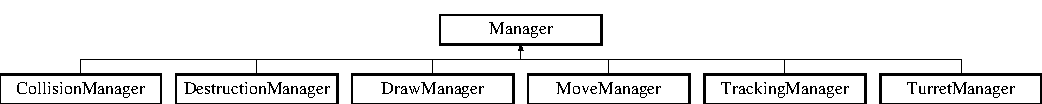
\includegraphics[height=1.382716cm]{class_manager}
\end{center}
\end{figure}
\subsection*{Public Member Functions}
\begin{DoxyCompactItemize}
\item 
\hyperlink{class_manager_a1658ff9f18e38ccd9cb8b0b371b9c20b}{Manager} ()
\begin{DoxyCompactList}\small\item\em Constructor for \hyperlink{class_manager}{Manager}. \end{DoxyCompactList}\item 
\hypertarget{class_manager_a322cad25d7007438b3a043ad02253d29}{virtual \hyperlink{class_manager_a322cad25d7007438b3a043ad02253d29}{$\sim$\+Manager} ()}\label{class_manager_a322cad25d7007438b3a043ad02253d29}

\begin{DoxyCompactList}\small\item\em Destructor. \end{DoxyCompactList}\end{DoxyCompactItemize}


\subsection{Detailed Description}


Definition at line 19 of file Manager.\+h.



\subsection{Constructor \& Destructor Documentation}
\hypertarget{class_manager_a1658ff9f18e38ccd9cb8b0b371b9c20b}{\index{Manager@{Manager}!Manager@{Manager}}
\index{Manager@{Manager}!Manager@{Manager}}
\subsubsection[{Manager}]{\setlength{\rightskip}{0pt plus 5cm}Manager\+::\+Manager (
\begin{DoxyParamCaption}
{}
\end{DoxyParamCaption}
)}}\label{class_manager_a1658ff9f18e38ccd9cb8b0b371b9c20b}


Constructor for \hyperlink{class_manager}{Manager}. 

/file \hyperlink{_manager_8cpp_source}{Manager.\+cpp} /author Daniel Holmes \& Jonathan Gerrand /date 8 September 2014 /brief Implementation for \hyperlink{class_manager}{Manager} class 

Definition at line 10 of file Manager.\+cpp.



The documentation for this class was generated from the following files\+:\begin{DoxyCompactItemize}
\item 
\hyperlink{_manager_8h}{Manager.\+h}\item 
Manager.\+cpp\end{DoxyCompactItemize}

\hypertarget{class_manager_test_assistant}{\section{Manager\+Test\+Assistant Class Reference}
\label{class_manager_test_assistant}\index{Manager\+Test\+Assistant@{Manager\+Test\+Assistant}}
}
\subsection*{Public Member Functions}
\begin{DoxyCompactItemize}
\item 
\hypertarget{class_manager_test_assistant_aba7ce13afa76fd729f46247edc4a73a5}{std\+::shared\+\_\+ptr$<$ \hyperlink{class_deletable}{Deletable} $>$ {\bfseries create\+Deletable\+Entity\+Shared\+Pointer} (const entity\+\_\+type entity)}\label{class_manager_test_assistant_aba7ce13afa76fd729f46247edc4a73a5}

\end{DoxyCompactItemize}


\subsection{Detailed Description}


Definition at line 19 of file Manager\+Test\+Assistant.\+h.



The documentation for this class was generated from the following files\+:\begin{DoxyCompactItemize}
\item 
\hyperlink{_manager_test_assistant_8h}{Manager\+Test\+Assistant.\+h}\item 
\hyperlink{_manager_test_assistant_8cpp}{Manager\+Test\+Assistant.\+cpp}\end{DoxyCompactItemize}

\hypertarget{class_mine}{\section{Mine Class Reference}
\label{class_mine}\index{Mine@{Mine}}
}
Inheritance diagram for Mine\+:\begin{figure}[H]
\begin{center}
\leavevmode
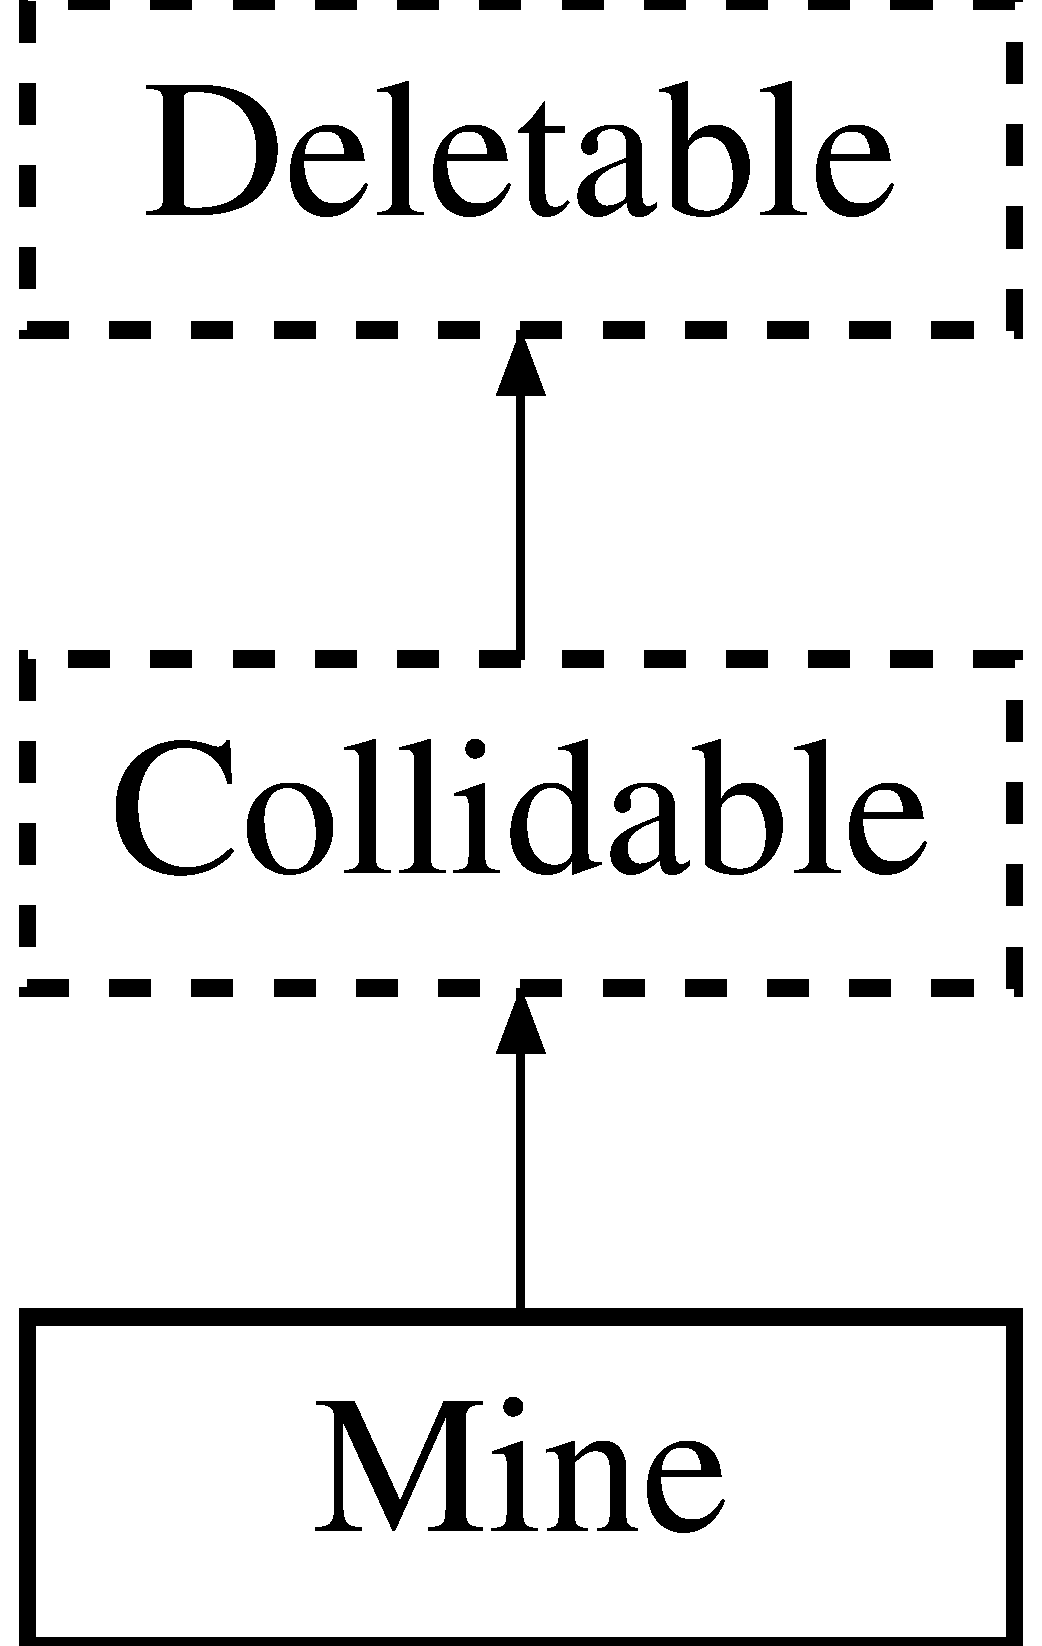
\includegraphics[height=3.000000cm]{class_mine}
\end{center}
\end{figure}
\subsection*{Public Member Functions}
\begin{DoxyCompactItemize}
\item 
\hyperlink{class_mine_ae3d52389f68d1f458e6240a44cbfd85a}{Mine} (float position\+X, float position\+Y, entity\+\_\+type mine\+Owner)
\begin{DoxyCompactList}\small\item\em \hyperlink{class_mine}{Mine} entity constructor. \end{DoxyCompactList}\item 
\hypertarget{class_mine_af435cf100fe7f89e998ec2f7ad40faa1}{virtual const entity\+\_\+type \& \hyperlink{class_mine_af435cf100fe7f89e998ec2f7ad40faa1}{get\+Type} () const }\label{class_mine_af435cf100fe7f89e998ec2f7ad40faa1}

\begin{DoxyCompactList}\small\item\em \hyperlink{class_mine}{Mine} is able to provide its identification. \end{DoxyCompactList}\item 
\hypertarget{class_mine_a36b2ba160a413d45c9743447f075e99e}{virtual const \hyperlink{structrect__corners}{rect\+\_\+corners} \& \hyperlink{class_mine_a36b2ba160a413d45c9743447f075e99e}{get\+Bounding\+Box} ()}\label{class_mine_a36b2ba160a413d45c9743447f075e99e}

\begin{DoxyCompactList}\small\item\em Provide the bounding box for the mine entity. \end{DoxyCompactList}\item 
\hypertarget{class_mine_a94667c68518d45d9c841501924a83612}{virtual const \hyperlink{structrect__corners}{rect\+\_\+corners} \& \hyperlink{class_mine_a94667c68518d45d9c841501924a83612}{get\+Aligned\+Bounding\+Box} ()}\label{class_mine_a94667c68518d45d9c841501924a83612}

\begin{DoxyCompactList}\small\item\em Get Axis Aligned bounding box of entity. \end{DoxyCompactList}\item 
virtual void \hyperlink{class_mine_a859fd28c2c57a37b22ec3b88806f1134}{set\+Unblocked} ()
\begin{DoxyCompactList}\small\item\em This function is not used by the mine. \end{DoxyCompactList}\item 
\hypertarget{class_mine_acf2add61f1763222f0d1a7333d2b0633}{virtual const int \hyperlink{class_mine_acf2add61f1763222f0d1a7333d2b0633}{set\+Blocked} (const blocked\+\_\+status obstruction\+\_\+type)}\label{class_mine_acf2add61f1763222f0d1a7333d2b0633}

\begin{DoxyCompactList}\small\item\em This function is not used by mine. \end{DoxyCompactList}\item 
\hypertarget{class_mine_a3a51fbecfcb177529bee4b7e13dd75e2}{virtual void \hyperlink{class_mine_a3a51fbecfcb177529bee4b7e13dd75e2}{set\+Collided} ()}\label{class_mine_a3a51fbecfcb177529bee4b7e13dd75e2}

\begin{DoxyCompactList}\small\item\em Set the colllision state of the mine. \end{DoxyCompactList}\item 
\hypertarget{class_mine_aa19d1827e837944d74fe02ad0fbeffc9}{virtual bool const \hyperlink{class_mine_aa19d1827e837944d74fe02ad0fbeffc9}{is\+Deleted} ()}\label{class_mine_aa19d1827e837944d74fe02ad0fbeffc9}

\begin{DoxyCompactList}\small\item\em Boolean state of the mine entities life. \end{DoxyCompactList}\item 
\hypertarget{class_mine_a904342dcd8d13f8489c91ed6ba09ec7b}{virtual const float \hyperlink{class_mine_a904342dcd8d13f8489c91ed6ba09ec7b}{get\+Draw\+Position\+X} ()}\label{class_mine_a904342dcd8d13f8489c91ed6ba09ec7b}

\begin{DoxyCompactList}\small\item\em Retrieve the \hyperlink{class_mine}{Mine} x Position. \end{DoxyCompactList}\item 
\hypertarget{class_mine_a8abe866b857f781f81b0b3b4e9ef7034}{virtual const float \hyperlink{class_mine_a8abe866b857f781f81b0b3b4e9ef7034}{get\+Draw\+Position\+Y} ()}\label{class_mine_a8abe866b857f781f81b0b3b4e9ef7034}

\begin{DoxyCompactList}\small\item\em Retrieve the \hyperlink{class_mine}{Mine} y Position. \end{DoxyCompactList}\item 
\hypertarget{class_mine_a5b6986a3a3ce5177879359a626cc994b}{virtual const float \hyperlink{class_mine_a5b6986a3a3ce5177879359a626cc994b}{get\+Draw\+Rotation} ()}\label{class_mine_a5b6986a3a3ce5177879359a626cc994b}

\begin{DoxyCompactList}\small\item\em Recieve the \hyperlink{class_mine}{Mine} rotation. \end{DoxyCompactList}\item 
\hypertarget{class_mine_abfde171f93b463d81d5b18f767a3a37c}{virtual \hyperlink{class_mine_abfde171f93b463d81d5b18f767a3a37c}{$\sim$\+Mine} ()}\label{class_mine_abfde171f93b463d81d5b18f767a3a37c}

\begin{DoxyCompactList}\small\item\em \hyperlink{class_mine}{Mine} object destructor. \end{DoxyCompactList}\end{DoxyCompactItemize}


\subsection{Detailed Description}


Definition at line 21 of file Mine.\+h.



\subsection{Constructor \& Destructor Documentation}
\hypertarget{class_mine_ae3d52389f68d1f458e6240a44cbfd85a}{\index{Mine@{Mine}!Mine@{Mine}}
\index{Mine@{Mine}!Mine@{Mine}}
\subsubsection[{Mine}]{\setlength{\rightskip}{0pt plus 5cm}Mine\+::\+Mine (
\begin{DoxyParamCaption}
\item[{float}]{position\+X, }
\item[{float}]{position\+Y, }
\item[{entity\+\_\+type}]{mine\+Owner}
\end{DoxyParamCaption}
)}}\label{class_mine_ae3d52389f68d1f458e6240a44cbfd85a}


\hyperlink{class_mine}{Mine} entity constructor. 

/file \hyperlink{_mine_8cpp_source}{Mine.\+cpp} /author Daniel Holmes \& Jonathan Gerrand /date 2 September 2014 /brief Implementation for \hyperlink{class_mine}{Mine} class 

Definition at line 11 of file Mine.\+cpp.



\subsection{Member Function Documentation}
\hypertarget{class_mine_a859fd28c2c57a37b22ec3b88806f1134}{\index{Mine@{Mine}!set\+Unblocked@{set\+Unblocked}}
\index{set\+Unblocked@{set\+Unblocked}!Mine@{Mine}}
\subsubsection[{set\+Unblocked}]{\setlength{\rightskip}{0pt plus 5cm}void Mine\+::set\+Unblocked (
\begin{DoxyParamCaption}
{}
\end{DoxyParamCaption}
)\hspace{0.3cm}{\ttfamily [virtual]}}}\label{class_mine_a859fd28c2c57a37b22ec3b88806f1134}


This function is not used by the mine. 

This function is not used by mine. 

Implements \hyperlink{class_collidable_a817d864d0640bc6bcb13bbecf14ddf31}{Collidable}.



Definition at line 50 of file Mine.\+cpp.



The documentation for this class was generated from the following files\+:\begin{DoxyCompactItemize}
\item 
\hyperlink{_mine_8h}{Mine.\+h}\item 
Mine.\+cpp\end{DoxyCompactItemize}

\hypertarget{class_missile}{\section{Missile Class Reference}
\label{class_missile}\index{Missile@{Missile}}
}
Inheritance diagram for Missile\+:\begin{figure}[H]
\begin{center}
\leavevmode
\includegraphics[height=3.000000cm]{class_missile}
\end{center}
\end{figure}
\subsection*{Public Member Functions}
\begin{DoxyCompactItemize}
\item 
\hypertarget{class_missile_a2f930ea9ba87704d2ba75b0299f698c2}{\hyperlink{class_missile_a2f930ea9ba87704d2ba75b0299f698c2}{Missile} (float position\+X, float position\+Y, float rotation, entity\+\_\+type missile\+Owner)}\label{class_missile_a2f930ea9ba87704d2ba75b0299f698c2}

\begin{DoxyCompactList}\small\item\em \hyperlink{class_missile}{Missile} object constructor. \end{DoxyCompactList}\item 
\hypertarget{class_missile_a67874a53d50f63065bf1f63803558513}{virtual const entity\+\_\+type \& \hyperlink{class_missile_a67874a53d50f63065bf1f63803558513}{get\+Type} () const }\label{class_missile_a67874a53d50f63065bf1f63803558513}

\begin{DoxyCompactList}\small\item\em Return the ownership and type of the \hyperlink{class_missile}{Missile} entity. \end{DoxyCompactList}\item 
\hypertarget{class_missile_a4b6a45a5129b97a6e5383123dffab0c3}{virtual void \hyperlink{class_missile_a4b6a45a5129b97a6e5383123dffab0c3}{move\+Forward} ()}\label{class_missile_a4b6a45a5129b97a6e5383123dffab0c3}

\begin{DoxyCompactList}\small\item\em Forward movement for a missile entity. \end{DoxyCompactList}\item 
\hypertarget{class_missile_a8d8348b91961ff0c163d7d24bd9599a8}{virtual void \hyperlink{class_missile_a8d8348b91961ff0c163d7d24bd9599a8}{move\+Backward} ()}\label{class_missile_a8d8348b91961ff0c163d7d24bd9599a8}

\begin{DoxyCompactList}\small\item\em Backward movement for a missile entity. \end{DoxyCompactList}\item 
\hypertarget{class_missile_a1c7ed80bd656b0af5b3872f4225978e3}{virtual void \hyperlink{class_missile_a1c7ed80bd656b0af5b3872f4225978e3}{rotate\+Left} ()}\label{class_missile_a1c7ed80bd656b0af5b3872f4225978e3}

\begin{DoxyCompactList}\small\item\em Left rotation for a missile entity. \end{DoxyCompactList}\item 
\hypertarget{class_missile_aeccfdf94a02fa86545296f4c38857ef8}{virtual void \hyperlink{class_missile_aeccfdf94a02fa86545296f4c38857ef8}{rotate\+Right} ()}\label{class_missile_aeccfdf94a02fa86545296f4c38857ef8}

\begin{DoxyCompactList}\small\item\em Right rotation for a missile entity. \end{DoxyCompactList}\item 
\hypertarget{class_missile_a6f9a14b7e2a2041fbccb566bf2a3b469}{virtual const \hyperlink{structrect__corners}{rect\+\_\+corners} \& \hyperlink{class_missile_a6f9a14b7e2a2041fbccb566bf2a3b469}{get\+Bounding\+Box} ()}\label{class_missile_a6f9a14b7e2a2041fbccb566bf2a3b469}

\begin{DoxyCompactList}\small\item\em Provide the bounding box for the missile entity. \end{DoxyCompactList}\item 
\hypertarget{class_missile_af2a9b1f8503cc2d322f5ab6ea788d393}{virtual const \hyperlink{structrect__corners}{rect\+\_\+corners} \& \hyperlink{class_missile_af2a9b1f8503cc2d322f5ab6ea788d393}{get\+Aligned\+Bounding\+Box} ()}\label{class_missile_af2a9b1f8503cc2d322f5ab6ea788d393}

\begin{DoxyCompactList}\small\item\em Get Axis Aligned bounding box of entity. \end{DoxyCompactList}\item 
\hypertarget{class_missile_a4f6e73f8d9f9723a777875efcb9edfa7}{virtual const int \hyperlink{class_missile_a4f6e73f8d9f9723a777875efcb9edfa7}{set\+Blocked} (const blocked\+\_\+status obstruction\+\_\+type)}\label{class_missile_a4f6e73f8d9f9723a777875efcb9edfa7}

\begin{DoxyCompactList}\small\item\em Instruct the missile entity that it cannot move along its trajectory. \end{DoxyCompactList}\item 
virtual void \hyperlink{class_missile_af66d762c4401061f64bcf9b46343c967}{set\+Unblocked} ()
\begin{DoxyCompactList}\small\item\em Instruct the missile entity that it can move. \end{DoxyCompactList}\item 
\hypertarget{class_missile_a1a27cc48265f34e3298c780c37ca8a0e}{virtual void \hyperlink{class_missile_a1a27cc48265f34e3298c780c37ca8a0e}{set\+Collided} ()}\label{class_missile_a1a27cc48265f34e3298c780c37ca8a0e}

\begin{DoxyCompactList}\small\item\em Instruct the missile entity that it has collided with another object. \end{DoxyCompactList}\item 
\hypertarget{class_missile_a2c86874bf5e6bde8cb97f4ed1a07c3ea}{virtual const blocked\+\_\+status \hyperlink{class_missile_a2c86874bf5e6bde8cb97f4ed1a07c3ea}{is\+Blocked} ()}\label{class_missile_a2c86874bf5e6bde8cb97f4ed1a07c3ea}

\begin{DoxyCompactList}\small\item\em Determine the blocked state of the missile entity. \end{DoxyCompactList}\item 
\hypertarget{class_missile_a96c1240f08fed605ff9e908a0bea50e4}{virtual bool const \hyperlink{class_missile_a96c1240f08fed605ff9e908a0bea50e4}{is\+Deleted} ()}\label{class_missile_a96c1240f08fed605ff9e908a0bea50e4}

\begin{DoxyCompactList}\small\item\em Boolean state of the missile entity's life. \end{DoxyCompactList}\item 
virtual const float \hyperlink{class_missile_a8e8d526d7578cfbabbd5bf1bdb9727bc}{get\+Draw\+Position\+X} ()
\begin{DoxyCompactList}\small\item\em Retrieve the missile x Position. \end{DoxyCompactList}\item 
virtual const float \hyperlink{class_missile_ad609bee2bfaf610824f32c15430fa6d8}{get\+Draw\+Position\+Y} ()
\begin{DoxyCompactList}\small\item\em Retrieve the missile y Position. \end{DoxyCompactList}\item 
virtual const float \hyperlink{class_missile_ab606b0b4f38c821063f210625f926374}{get\+Draw\+Rotation} ()
\begin{DoxyCompactList}\small\item\em Receive the missile rotation. \end{DoxyCompactList}\item 
\hypertarget{class_missile_a5bff45d0243e353acdf610fdade02bb0}{virtual void \hyperlink{class_missile_a5bff45d0243e353acdf610fdade02bb0}{set\+Movement\+Direction} (const \hyperlink{_structures_8h_a0d0b88f27f3adf9452879b5d9f829026}{movement\+\_\+direction} Movement\+\_\+input)}\label{class_missile_a5bff45d0243e353acdf610fdade02bb0}

\begin{DoxyCompactList}\small\item\em Set the movement direction of the entity. \end{DoxyCompactList}\item 
\hypertarget{class_missile_ad42379e48a46ec3556056f98ce8bd912}{virtual \hyperlink{class_missile_ad42379e48a46ec3556056f98ce8bd912}{$\sim$\+Missile} ()}\label{class_missile_ad42379e48a46ec3556056f98ce8bd912}

\begin{DoxyCompactList}\small\item\em \hyperlink{class_missile}{Missile} object destructor. \end{DoxyCompactList}\end{DoxyCompactItemize}
\subsection*{Additional Inherited Members}


\subsection{Detailed Description}


Definition at line 24 of file Missile.\+h.



\subsection{Member Function Documentation}
\hypertarget{class_missile_a8e8d526d7578cfbabbd5bf1bdb9727bc}{\index{Missile@{Missile}!get\+Draw\+Position\+X@{get\+Draw\+Position\+X}}
\index{get\+Draw\+Position\+X@{get\+Draw\+Position\+X}!Missile@{Missile}}
\subsubsection[{get\+Draw\+Position\+X}]{\setlength{\rightskip}{0pt plus 5cm}const float Missile\+::get\+Draw\+Position\+X (
\begin{DoxyParamCaption}
{}
\end{DoxyParamCaption}
)\hspace{0.3cm}{\ttfamily [virtual]}}}\label{class_missile_a8e8d526d7578cfbabbd5bf1bdb9727bc}


Retrieve the missile x Position. 

Retrieve the \hyperlink{class_missile}{Missile} x Position. 

Implements \hyperlink{class_deletable_ac14ea0c5986d50ba3ba454f89c87b8fe}{Deletable}.



Definition at line 113 of file Missile.\+cpp.

\hypertarget{class_missile_ad609bee2bfaf610824f32c15430fa6d8}{\index{Missile@{Missile}!get\+Draw\+Position\+Y@{get\+Draw\+Position\+Y}}
\index{get\+Draw\+Position\+Y@{get\+Draw\+Position\+Y}!Missile@{Missile}}
\subsubsection[{get\+Draw\+Position\+Y}]{\setlength{\rightskip}{0pt plus 5cm}const float Missile\+::get\+Draw\+Position\+Y (
\begin{DoxyParamCaption}
{}
\end{DoxyParamCaption}
)\hspace{0.3cm}{\ttfamily [virtual]}}}\label{class_missile_ad609bee2bfaf610824f32c15430fa6d8}


Retrieve the missile y Position. 

Retrieve the \hyperlink{class_missile}{Missile} y Position. 

Implements \hyperlink{class_deletable_a2a88d7e40c56902a3d3d8f668e9d126d}{Deletable}.



Definition at line 119 of file Missile.\+cpp.

\hypertarget{class_missile_ab606b0b4f38c821063f210625f926374}{\index{Missile@{Missile}!get\+Draw\+Rotation@{get\+Draw\+Rotation}}
\index{get\+Draw\+Rotation@{get\+Draw\+Rotation}!Missile@{Missile}}
\subsubsection[{get\+Draw\+Rotation}]{\setlength{\rightskip}{0pt plus 5cm}const float Missile\+::get\+Draw\+Rotation (
\begin{DoxyParamCaption}
{}
\end{DoxyParamCaption}
)\hspace{0.3cm}{\ttfamily [virtual]}}}\label{class_missile_ab606b0b4f38c821063f210625f926374}


Receive the missile rotation. 

Recieve the \hyperlink{class_missile}{Missile} rotation. 

Implements \hyperlink{class_deletable_ad7061a6bef3efce030aa5abbc7646d47}{Deletable}.



Definition at line 126 of file Missile.\+cpp.

\hypertarget{class_missile_af66d762c4401061f64bcf9b46343c967}{\index{Missile@{Missile}!set\+Unblocked@{set\+Unblocked}}
\index{set\+Unblocked@{set\+Unblocked}!Missile@{Missile}}
\subsubsection[{set\+Unblocked}]{\setlength{\rightskip}{0pt plus 5cm}void Missile\+::set\+Unblocked (
\begin{DoxyParamCaption}
{}
\end{DoxyParamCaption}
)\hspace{0.3cm}{\ttfamily [virtual]}}}\label{class_missile_af66d762c4401061f64bcf9b46343c967}


Instruct the missile entity that it can move. 

Instruct the tank entity that it can move. 

Implements \hyperlink{class_collidable_a817d864d0640bc6bcb13bbecf14ddf31}{Collidable}.



Definition at line 89 of file Missile.\+cpp.



The documentation for this class was generated from the following files\+:\begin{DoxyCompactItemize}
\item 
\hyperlink{_missile_8h}{Missile.\+h}\item 
\hyperlink{_missile_8cpp}{Missile.\+cpp}\end{DoxyCompactItemize}

\hypertarget{class_movable}{\section{Movable Class Reference}
\label{class_movable}\index{Movable@{Movable}}
}
Inheritance diagram for Movable\+:\begin{figure}[H]
\begin{center}
\leavevmode
\includegraphics[height=3.000000cm]{class_movable}
\end{center}
\end{figure}
\subsection*{Public Member Functions}
\begin{DoxyCompactItemize}
\item 
\hypertarget{class_movable_a053cf48796f1aef5b6f6cb4c6b22db78}{\hyperlink{class_movable_a053cf48796f1aef5b6f6cb4c6b22db78}{Movable} ()}\label{class_movable_a053cf48796f1aef5b6f6cb4c6b22db78}

\begin{DoxyCompactList}\small\item\em Constructor. \end{DoxyCompactList}\item 
\hypertarget{class_movable_adefaf61339698c5efec597529bf89310}{virtual void \hyperlink{class_movable_adefaf61339698c5efec597529bf89310}{move\+Forward} ()=0}\label{class_movable_adefaf61339698c5efec597529bf89310}

\begin{DoxyCompactList}\small\item\em Move a moveable entity forward. \end{DoxyCompactList}\item 
\hypertarget{class_movable_a9c03e7ac263902159579d7f83e9b6dee}{virtual void \hyperlink{class_movable_a9c03e7ac263902159579d7f83e9b6dee}{move\+Backward} ()=0}\label{class_movable_a9c03e7ac263902159579d7f83e9b6dee}

\begin{DoxyCompactList}\small\item\em Move a moveable entity backward. \end{DoxyCompactList}\item 
\hypertarget{class_movable_a422b71ade02b9034600f51bc55d58c90}{virtual void \hyperlink{class_movable_a422b71ade02b9034600f51bc55d58c90}{rotate\+Left} ()=0}\label{class_movable_a422b71ade02b9034600f51bc55d58c90}

\begin{DoxyCompactList}\small\item\em Rotate a moveable entity left. \end{DoxyCompactList}\item 
\hypertarget{class_movable_a821480cb8ffd047b39a907c6cf07dd84}{virtual void \hyperlink{class_movable_a821480cb8ffd047b39a907c6cf07dd84}{rotate\+Right} ()=0}\label{class_movable_a821480cb8ffd047b39a907c6cf07dd84}

\begin{DoxyCompactList}\small\item\em Rotate a moveable entity right. \end{DoxyCompactList}\item 
\hypertarget{class_movable_a40db320f27f5be1882553298677702c8}{virtual const blocked\+\_\+status \hyperlink{class_movable_a40db320f27f5be1882553298677702c8}{is\+Blocked} ()=0}\label{class_movable_a40db320f27f5be1882553298677702c8}

\begin{DoxyCompactList}\small\item\em Check state of entity to see number of times it has been blocked by another object. \end{DoxyCompactList}\item 
\hypertarget{class_movable_a0bb485f10776845305a683ed5e2ba1fc}{virtual void \hyperlink{class_movable_a0bb485f10776845305a683ed5e2ba1fc}{set\+Movement\+Direction} (const \hyperlink{_structures_8h_a0d0b88f27f3adf9452879b5d9f829026}{movement\+\_\+direction} Movement\+\_\+input)=0}\label{class_movable_a0bb485f10776845305a683ed5e2ba1fc}

\begin{DoxyCompactList}\small\item\em Set the movement direction of the entity. \end{DoxyCompactList}\item 
\hypertarget{class_movable_ae629c22458180741deb4b67b9523c794}{virtual \hyperlink{class_movable_ae629c22458180741deb4b67b9523c794}{$\sim$\+Movable} ()=0}\label{class_movable_ae629c22458180741deb4b67b9523c794}

\begin{DoxyCompactList}\small\item\em Destructor. \end{DoxyCompactList}\end{DoxyCompactItemize}
\subsection*{Static Protected Attributes}
\begin{DoxyCompactItemize}
\item 
\hypertarget{class_movable_aff7e2a3e3d5a6059c4fe138aa47dc048}{static const int \hyperlink{class_movable_aff7e2a3e3d5a6059c4fe138aa47dc048}{\+\_\+missile\+Movement\+Speed} = 8}\label{class_movable_aff7e2a3e3d5a6059c4fe138aa47dc048}

\begin{DoxyCompactList}\small\item\em Define the movement speed of a missile entity. \end{DoxyCompactList}\item 
\hypertarget{class_movable_a54cb7d3465cc78ad7d8b2f7c2d842732}{static const int \hyperlink{class_movable_a54cb7d3465cc78ad7d8b2f7c2d842732}{\+\_\+tank\+Movement\+Speed} = 3}\label{class_movable_a54cb7d3465cc78ad7d8b2f7c2d842732}

\begin{DoxyCompactList}\small\item\em Define the movement speed of a tank entity. \end{DoxyCompactList}\item 
\hypertarget{class_movable_afde3611f73293d67497a39fed061e3a8}{static const int \hyperlink{class_movable_afde3611f73293d67497a39fed061e3a8}{\+\_\+missile\+Rotation\+Speed} = 45}\label{class_movable_afde3611f73293d67497a39fed061e3a8}

\begin{DoxyCompactList}\small\item\em Define the rotation speed of a missile entity. \end{DoxyCompactList}\item 
\hypertarget{class_movable_ab4ad35a0057bdbc80385c67bec5f1a60}{static const int \hyperlink{class_movable_ab4ad35a0057bdbc80385c67bec5f1a60}{\+\_\+tank\+Rotation\+Speed} = 5}\label{class_movable_ab4ad35a0057bdbc80385c67bec5f1a60}

\begin{DoxyCompactList}\small\item\em Define the rotatioin speed of a tank entity. \end{DoxyCompactList}\end{DoxyCompactItemize}


\subsection{Detailed Description}


Definition at line 21 of file Movable.\+h.



The documentation for this class was generated from the following files\+:\begin{DoxyCompactItemize}
\item 
Movable.\+h\item 
Movable.\+cpp\end{DoxyCompactItemize}

\hypertarget{class_move_manager}{\section{Move\+Manager Class Reference}
\label{class_move_manager}\index{Move\+Manager@{Move\+Manager}}
}
Inheritance diagram for Move\+Manager\+:\begin{figure}[H]
\begin{center}
\leavevmode
\includegraphics[height=2.000000cm]{class_move_manager}
\end{center}
\end{figure}
\subsection*{Public Member Functions}
\begin{DoxyCompactItemize}
\item 
\hyperlink{class_move_manager_a57ac62af15a2d9f9ed9b9ae96ea7900f}{Move\+Manager} ()
\begin{DoxyCompactList}\small\item\em Constructor. \end{DoxyCompactList}\item 
\hypertarget{class_move_manager_a1e21cd4f542f801e84b57fd5f11f1154}{void \hyperlink{class_move_manager_a1e21cd4f542f801e84b57fd5f11f1154}{manage} (const \hyperlink{class_action_data}{Action\+Data} \&action\+\_\+data\+\_\+container)}\label{class_move_manager_a1e21cd4f542f801e84b57fd5f11f1154}

\begin{DoxyCompactList}\small\item\em Move all movable entities within the world. \end{DoxyCompactList}\item 
\hypertarget{class_move_manager_a9f49f128a880d4f94c529c6aafab880e}{void \hyperlink{class_move_manager_a9f49f128a880d4f94c529c6aafab880e}{add\+New\+Entity} (std\+::weak\+\_\+ptr$<$ \hyperlink{class_movable}{Movable} $>$ new\+\_\+entity)}\label{class_move_manager_a9f49f128a880d4f94c529c6aafab880e}

\begin{DoxyCompactList}\small\item\em Add Movable-\/type shared\+\_\+ptr's to the Move\+Managers internal data members. \end{DoxyCompactList}\item 
\hypertarget{class_move_manager_a1de20c7414d1511c5b3a58196a557d94}{virtual \hyperlink{class_move_manager_a1de20c7414d1511c5b3a58196a557d94}{$\sim$\+Move\+Manager} ()}\label{class_move_manager_a1de20c7414d1511c5b3a58196a557d94}

\begin{DoxyCompactList}\small\item\em Destructor for \hyperlink{class_move_manager}{Move\+Manager}. \end{DoxyCompactList}\end{DoxyCompactItemize}


\subsection{Detailed Description}


Definition at line 19 of file Move\+Manager.\+h.



\subsection{Constructor \& Destructor Documentation}
\hypertarget{class_move_manager_a57ac62af15a2d9f9ed9b9ae96ea7900f}{\index{Move\+Manager@{Move\+Manager}!Move\+Manager@{Move\+Manager}}
\index{Move\+Manager@{Move\+Manager}!Move\+Manager@{Move\+Manager}}
\subsubsection[{Move\+Manager}]{\setlength{\rightskip}{0pt plus 5cm}Move\+Manager\+::\+Move\+Manager (
\begin{DoxyParamCaption}
{}
\end{DoxyParamCaption}
)}}\label{class_move_manager_a57ac62af15a2d9f9ed9b9ae96ea7900f}


Constructor. 

/file \hyperlink{_move_manager_8cpp_source}{Move\+Manager.\+cpp} /author Daniel Holmes \& Jonathan Gerrand /date 2 September 2014 /brief Implementation for \hyperlink{class_move_manager}{Move\+Manager} class 

Definition at line 10 of file Move\+Manager.\+cpp.



The documentation for this class was generated from the following files\+:\begin{DoxyCompactItemize}
\item 
\hyperlink{_move_manager_8h}{Move\+Manager.\+h}\item 
Move\+Manager.\+cpp\end{DoxyCompactItemize}

\hypertarget{class_orientation}{\section{Orientation Class Reference}
\label{class_orientation}\index{Orientation@{Orientation}}
}
\subsection*{Public Member Functions}
\begin{DoxyCompactItemize}
\item 
\hypertarget{class_orientation_ae2df457b68375ea4915f7fa1c161b116}{\hyperlink{class_orientation_ae2df457b68375ea4915f7fa1c161b116}{Orientation} (float origin\+\_\+x, float origin\+\_\+y, float width, float height, float rotation, bool controllable)}\label{class_orientation_ae2df457b68375ea4915f7fa1c161b116}

\begin{DoxyCompactList}\small\item\em Constructor that initialises all data members of the class. \end{DoxyCompactList}\item 
\hypertarget{class_orientation_a4d6b853f2ac00965d29e5bc36b94c949}{const float \hyperlink{class_orientation_a4d6b853f2ac00965d29e5bc36b94c949}{get\+Origin\+X} ()}\label{class_orientation_a4d6b853f2ac00965d29e5bc36b94c949}

\begin{DoxyCompactList}\small\item\em Returns the entity origin x value. \end{DoxyCompactList}\item 
\hypertarget{class_orientation_ae60c88b0525d6e536a1a068d3a99f74c}{const float \hyperlink{class_orientation_ae60c88b0525d6e536a1a068d3a99f74c}{get\+Origin\+Y} ()}\label{class_orientation_ae60c88b0525d6e536a1a068d3a99f74c}

\begin{DoxyCompactList}\small\item\em Returns the entity origin y value. \end{DoxyCompactList}\item 
\hypertarget{class_orientation_adf3e031c3ce102233782e6fdeb976ef3}{const float \hyperlink{class_orientation_adf3e031c3ce102233782e6fdeb976ef3}{get\+Width} ()}\label{class_orientation_adf3e031c3ce102233782e6fdeb976ef3}

\begin{DoxyCompactList}\small\item\em Returns the entity width. \end{DoxyCompactList}\item 
\hypertarget{class_orientation_af7c9a2f7547c76ce2408ac6fefacf9e1}{const float \hyperlink{class_orientation_af7c9a2f7547c76ce2408ac6fefacf9e1}{get\+Height} ()}\label{class_orientation_af7c9a2f7547c76ce2408ac6fefacf9e1}

\begin{DoxyCompactList}\small\item\em Returns the entity height. \end{DoxyCompactList}\item 
\hypertarget{class_orientation_ab3568e037a7dc7799d557f2bc6a3cf7d}{const float \hyperlink{class_orientation_ab3568e037a7dc7799d557f2bc6a3cf7d}{get\+Rotation} ()}\label{class_orientation_ab3568e037a7dc7799d557f2bc6a3cf7d}

\begin{DoxyCompactList}\small\item\em Returns the entity rotation. \end{DoxyCompactList}\item 
\hypertarget{class_orientation_a1b5cd490e5bbbe2b8d683be389dbcbbe}{void \hyperlink{class_orientation_a1b5cd490e5bbbe2b8d683be389dbcbbe}{set\+Width} (const float width)}\label{class_orientation_a1b5cd490e5bbbe2b8d683be389dbcbbe}

\begin{DoxyCompactList}\small\item\em Set the Width Value. \end{DoxyCompactList}\item 
\hypertarget{class_orientation_a1adca89bc32128e2ca1cb937357f5006}{void \hyperlink{class_orientation_a1adca89bc32128e2ca1cb937357f5006}{set\+Height} (const float height)}\label{class_orientation_a1adca89bc32128e2ca1cb937357f5006}

\begin{DoxyCompactList}\small\item\em Set the Height Value. \end{DoxyCompactList}\item 
\hypertarget{class_orientation_ae1c8122591724b1b3bfcb0026b76e809}{void \hyperlink{class_orientation_ae1c8122591724b1b3bfcb0026b76e809}{move} (float movement\+\_\+in\+\_\+x, float movement\+\_\+in\+\_\+y)}\label{class_orientation_ae1c8122591724b1b3bfcb0026b76e809}

\begin{DoxyCompactList}\small\item\em Move the entity by a distance. \end{DoxyCompactList}\item 
\hypertarget{class_orientation_aa9e115b7f4ab487e3af532592416b247}{void \hyperlink{class_orientation_aa9e115b7f4ab487e3af532592416b247}{rotate} (float angle)}\label{class_orientation_aa9e115b7f4ab487e3af532592416b247}

\begin{DoxyCompactList}\small\item\em Rotate the entity by a supplied angle. \end{DoxyCompactList}\item 
\hypertarget{class_orientation_a478512ba497cd75f11be3aa3177cca6a}{void \hyperlink{class_orientation_a478512ba497cd75f11be3aa3177cca6a}{set\+Move\+Direction} (const \hyperlink{_structures_8h_a0d0b88f27f3adf9452879b5d9f829026}{movement\+\_\+direction})}\label{class_orientation_a478512ba497cd75f11be3aa3177cca6a}

\begin{DoxyCompactList}\small\item\em Used to set the state of future collision detection. \end{DoxyCompactList}\item 
\hypertarget{class_orientation_a950dfe84e548582d8c3c573b5ff5fe42}{\hyperlink{structrect__corners}{rect\+\_\+corners} \& \hyperlink{class_orientation_a950dfe84e548582d8c3c573b5ff5fe42}{get\+Global\+Bounds} ()}\label{class_orientation_a950dfe84e548582d8c3c573b5ff5fe42}

\begin{DoxyCompactList}\small\item\em Retrieve Rectangular co-\/ordinates for collision detection. \end{DoxyCompactList}\item 
\hypertarget{class_orientation_a5cc606289f774c8561af98d183586199}{const \hyperlink{structrect__corners}{rect\+\_\+corners} \& \hyperlink{class_orientation_a5cc606289f774c8561af98d183586199}{get\+Aligned\+Global\+Bounds} ()}\label{class_orientation_a5cc606289f774c8561af98d183586199}

\begin{DoxyCompactList}\small\item\em Retrieve Rectangular co-\/ordinated for collision detection (Non-\/rotated) \end{DoxyCompactList}\item 
\hypertarget{class_orientation_a8c96df6f0b3b9a9edc7f9a0a9cc10741}{virtual \hyperlink{class_orientation_a8c96df6f0b3b9a9edc7f9a0a9cc10741}{$\sim$\+Orientation} ()}\label{class_orientation_a8c96df6f0b3b9a9edc7f9a0a9cc10741}

\begin{DoxyCompactList}\small\item\em Destructor. \end{DoxyCompactList}\item 
\hypertarget{class_orientation_a0195b81c78baadd074301bc019d11db8}{bool \hyperlink{class_orientation_a0195b81c78baadd074301bc019d11db8}{operator==} (\hyperlink{class_orientation}{Orientation} \&rhs) const }\label{class_orientation_a0195b81c78baadd074301bc019d11db8}

\begin{DoxyCompactList}\small\item\em Equality operator overload for testing. \end{DoxyCompactList}\end{DoxyCompactItemize}


\subsection{Detailed Description}


Definition at line 17 of file Orientation.\+h.



The documentation for this class was generated from the following files\+:\begin{DoxyCompactItemize}
\item 
\hyperlink{_orientation_8h}{Orientation.\+h}\item 
\hyperlink{_orientation_8cpp}{Orientation.\+cpp}\end{DoxyCompactItemize}

\hypertarget{structrect__corners}{\section{rect\-\_\-corners Struct Reference}
\label{structrect__corners}\index{rect\-\_\-corners@{rect\-\_\-corners}}
}


Contains x and y corners of a rectangle, used in the algorithm for collision detection.  




{\ttfamily \#include $<$Structures.\-h$>$}

\subsection*{Public Attributes}
\begin{DoxyCompactItemize}
\item 
\hyperlink{structcoordinate}{coordinate} \hyperlink{structrect__corners_a48cd191550e65bd24a7d8018c7eefd53}{upper\-\_\-left}
\item 
\hyperlink{structcoordinate}{coordinate} \hyperlink{structrect__corners_a631310450f151fd6c92132d5d7216259}{upper\-\_\-right}
\item 
\hyperlink{structcoordinate}{coordinate} \hyperlink{structrect__corners_a2960e4888d6a9621429044e426950bc8}{lower\-\_\-left}
\item 
\hyperlink{structcoordinate}{coordinate} \hyperlink{structrect__corners_aa499428b9c692d61e1b43d059156a5af}{lower\-\_\-right}
\end{DoxyCompactItemize}


\subsection{Detailed Description}
Contains x and y corners of a rectangle, used in the algorithm for collision detection. 

Definition at line 93 of file Structures.\-h.



\subsection{Member Data Documentation}
\hypertarget{structrect__corners_a2960e4888d6a9621429044e426950bc8}{\index{rect\-\_\-corners@{rect\-\_\-corners}!lower\-\_\-left@{lower\-\_\-left}}
\index{lower\-\_\-left@{lower\-\_\-left}!rect_corners@{rect\-\_\-corners}}
\subsubsection[{lower\-\_\-left}]{\setlength{\rightskip}{0pt plus 5cm}{\bf coordinate} rect\-\_\-corners\-::lower\-\_\-left}}\label{structrect__corners_a2960e4888d6a9621429044e426950bc8}


Definition at line 97 of file Structures.\-h.



Referenced by Geometry\-Engine\-::calculate\-Vector\-Projections(), Orientation\-::get\-Aligned\-Global\-Bounds(), Geometry\-Engine\-::is\-Collision(), Geometry\-Engine\-::is\-In\-Line\-Of\-Fire(), Geometry\-Engine\-::is\-Valid\-Rect\-Entity(), Geometry\-Engine\-::right\-Points\-Left\-Of\-Object(), Orientation\-::set\-Global\-Bounds(), T\-E\-S\-T(), and Geometry\-Engine\-::upper\-Points\-Below\-Bottom\-Of\-Object().

\hypertarget{structrect__corners_aa499428b9c692d61e1b43d059156a5af}{\index{rect\-\_\-corners@{rect\-\_\-corners}!lower\-\_\-right@{lower\-\_\-right}}
\index{lower\-\_\-right@{lower\-\_\-right}!rect_corners@{rect\-\_\-corners}}
\subsubsection[{lower\-\_\-right}]{\setlength{\rightskip}{0pt plus 5cm}{\bf coordinate} rect\-\_\-corners\-::lower\-\_\-right}}\label{structrect__corners_aa499428b9c692d61e1b43d059156a5af}


Definition at line 98 of file Structures.\-h.



Referenced by Geometry\-Engine\-::calculate\-Vector\-Projections(), Orientation\-::get\-Aligned\-Global\-Bounds(), Geometry\-Engine\-::is\-Collision(), Geometry\-Engine\-::is\-In\-Line\-Of\-Fire(), Geometry\-Engine\-::is\-Valid\-Rect\-Entity(), Geometry\-Engine\-::left\-Points\-Right\-Of\-Object(), Orientation\-::set\-Global\-Bounds(), T\-E\-S\-T(), and Geometry\-Engine\-::upper\-Points\-Below\-Bottom\-Of\-Object().

\hypertarget{structrect__corners_a48cd191550e65bd24a7d8018c7eefd53}{\index{rect\-\_\-corners@{rect\-\_\-corners}!upper\-\_\-left@{upper\-\_\-left}}
\index{upper\-\_\-left@{upper\-\_\-left}!rect_corners@{rect\-\_\-corners}}
\subsubsection[{upper\-\_\-left}]{\setlength{\rightskip}{0pt plus 5cm}{\bf coordinate} rect\-\_\-corners\-::upper\-\_\-left}}\label{structrect__corners_a48cd191550e65bd24a7d8018c7eefd53}


Definition at line 95 of file Structures.\-h.



Referenced by Geometry\-Engine\-::calculate\-Vector\-Projections(), Orientation\-::get\-Aligned\-Global\-Bounds(), Geometry\-Engine\-::is\-Collision(), Geometry\-Engine\-::is\-In\-Line\-Of\-Fire(), Geometry\-Engine\-::is\-Valid\-Rect\-Entity(), Geometry\-Engine\-::lowwer\-Points\-Above\-Top\-Of\-Object(), Geometry\-Engine\-::right\-Points\-Left\-Of\-Object(), Orientation\-::set\-Global\-Bounds(), and T\-E\-S\-T().

\hypertarget{structrect__corners_a631310450f151fd6c92132d5d7216259}{\index{rect\-\_\-corners@{rect\-\_\-corners}!upper\-\_\-right@{upper\-\_\-right}}
\index{upper\-\_\-right@{upper\-\_\-right}!rect_corners@{rect\-\_\-corners}}
\subsubsection[{upper\-\_\-right}]{\setlength{\rightskip}{0pt plus 5cm}{\bf coordinate} rect\-\_\-corners\-::upper\-\_\-right}}\label{structrect__corners_a631310450f151fd6c92132d5d7216259}


Definition at line 96 of file Structures.\-h.



Referenced by Geometry\-Engine\-::calculate\-Vector\-Projections(), Orientation\-::get\-Aligned\-Global\-Bounds(), Geometry\-Engine\-::is\-Collision(), Geometry\-Engine\-::is\-In\-Line\-Of\-Fire(), Geometry\-Engine\-::is\-Valid\-Rect\-Entity(), Geometry\-Engine\-::left\-Points\-Right\-Of\-Object(), Geometry\-Engine\-::lowwer\-Points\-Above\-Top\-Of\-Object(), Orientation\-::set\-Global\-Bounds(), and T\-E\-S\-T().



The documentation for this struct was generated from the following file\-:\begin{DoxyCompactItemize}
\item 
\hyperlink{Structures_8h}{Structures.\-h}\end{DoxyCompactItemize}

\hypertarget{structsprite__draw__info}{\section{sprite\+\_\+draw\+\_\+info Struct Reference}
\label{structsprite__draw__info}\index{sprite\+\_\+draw\+\_\+info@{sprite\+\_\+draw\+\_\+info}}
}


Used for passing information from draw manager to display.  




{\ttfamily \#include $<$Structures.\+h$>$}

\subsection*{Public Attributes}
\begin{DoxyCompactItemize}
\item 
\hypertarget{structsprite__draw__info_a7c12e335ba1fc83156a05a568d38a179}{\hyperlink{structcoordinate}{coordinate} {\bfseries origin}}\label{structsprite__draw__info_a7c12e335ba1fc83156a05a568d38a179}

\item 
\hypertarget{structsprite__draw__info_acf0a863cddf497e364e3cdc9c46b8564}{\hyperlink{structcoordinate}{coordinate} {\bfseries draw\+\_\+pos}}\label{structsprite__draw__info_acf0a863cddf497e364e3cdc9c46b8564}

\item 
\hypertarget{structsprite__draw__info_a41292dd9fa6ca00d553a6c93f18e2a40}{float {\bfseries rotation}}\label{structsprite__draw__info_a41292dd9fa6ca00d553a6c93f18e2a40}

\end{DoxyCompactItemize}


\subsection{Detailed Description}
Used for passing information from draw manager to display. 

Definition at line 117 of file Structures.\+h.



The documentation for this struct was generated from the following file\+:\begin{DoxyCompactItemize}
\item 
\hyperlink{_structures_8h}{Structures.\+h}\end{DoxyCompactItemize}

\hypertarget{class_sprite_dimensions}{\section{Sprite\+Dimensions Class Reference}
\label{class_sprite_dimensions}\index{Sprite\+Dimensions@{Sprite\+Dimensions}}
}
\subsection*{Public Member Functions}
\begin{DoxyCompactItemize}
\item 
\hypertarget{class_sprite_dimensions_a5ae560281c00f763641653b9e121614f}{\hyperlink{class_sprite_dimensions_a5ae560281c00f763641653b9e121614f}{Sprite\+Dimensions} ()}\label{class_sprite_dimensions_a5ae560281c00f763641653b9e121614f}

\begin{DoxyCompactList}\small\item\em Constructor. \end{DoxyCompactList}\item 
\hypertarget{class_sprite_dimensions_a9309ef0f1d831d1ca4e1c65fda492c5f}{\hyperlink{class_sprite_dimensions_a9309ef0f1d831d1ca4e1c65fda492c5f}{$\sim$\+Sprite\+Dimensions} ()}\label{class_sprite_dimensions_a9309ef0f1d831d1ca4e1c65fda492c5f}

\begin{DoxyCompactList}\small\item\em Destructor. \end{DoxyCompactList}\end{DoxyCompactItemize}
\subsection*{Public Attributes}
\begin{DoxyCompactItemize}
\item 
\hypertarget{class_sprite_dimensions_a9d7ddd6f707798f86ced573e28f9eea0}{const float {\bfseries tank\+\_\+sprite\+\_\+x}}\label{class_sprite_dimensions_a9d7ddd6f707798f86ced573e28f9eea0}

\item 
\hypertarget{class_sprite_dimensions_a0c406c32caf5ea7841c763100dd83ecf}{const float {\bfseries missile\+\_\+sprite\+\_\+x}}\label{class_sprite_dimensions_a0c406c32caf5ea7841c763100dd83ecf}

\item 
\hypertarget{class_sprite_dimensions_af7f442b00b4a2d9d8b9ad47371a0018f}{const float {\bfseries mine\+\_\+sprite\+\_\+x}}\label{class_sprite_dimensions_af7f442b00b4a2d9d8b9ad47371a0018f}

\item 
\hypertarget{class_sprite_dimensions_a69ff9ddd57b6fe4af120278bcece5439}{const float {\bfseries map\+\_\+sprite\+\_\+x}}\label{class_sprite_dimensions_a69ff9ddd57b6fe4af120278bcece5439}

\item 
\hypertarget{class_sprite_dimensions_abcc491d376f31d36013e4f2396dbc408}{const float {\bfseries barrier\+\_\+sprite\+\_\+x}}\label{class_sprite_dimensions_abcc491d376f31d36013e4f2396dbc408}

\item 
\hypertarget{class_sprite_dimensions_ad876e1e5dea420fe80462709c8ec2d5c}{const float {\bfseries turret\+\_\+sprite\+\_\+x}}\label{class_sprite_dimensions_ad876e1e5dea420fe80462709c8ec2d5c}

\item 
\hypertarget{class_sprite_dimensions_abe1930e59ce44b9bdc0e6b363b668f7d}{const float {\bfseries tank\+\_\+sprite\+\_\+y}}\label{class_sprite_dimensions_abe1930e59ce44b9bdc0e6b363b668f7d}

\item 
\hypertarget{class_sprite_dimensions_adcf501d11ae383d24cbbe5b526585f86}{const float {\bfseries missile\+\_\+sprite\+\_\+y}}\label{class_sprite_dimensions_adcf501d11ae383d24cbbe5b526585f86}

\item 
\hypertarget{class_sprite_dimensions_a256b5245430fc54ae2cace272260dbe1}{const float {\bfseries mine\+\_\+sprite\+\_\+y}}\label{class_sprite_dimensions_a256b5245430fc54ae2cace272260dbe1}

\item 
\hypertarget{class_sprite_dimensions_a33014d94b303afe312e1a4b2fb5e437f}{const float {\bfseries map\+\_\+sprite\+\_\+y}}\label{class_sprite_dimensions_a33014d94b303afe312e1a4b2fb5e437f}

\item 
\hypertarget{class_sprite_dimensions_abad79766e2254e365d3455b3471a5d0a}{const float {\bfseries barrier\+\_\+sprite\+\_\+y}}\label{class_sprite_dimensions_abad79766e2254e365d3455b3471a5d0a}

\item 
\hypertarget{class_sprite_dimensions_a1b808c73bd915776ec6b8c10120adeae}{const float {\bfseries turret\+\_\+sprite\+\_\+y}}\label{class_sprite_dimensions_a1b808c73bd915776ec6b8c10120adeae}

\item 
\hypertarget{class_sprite_dimensions_a01c7c9dc1498f3336671b1ca697a7342}{const float {\bfseries mine\+\_\+creation\+\_\+offset}}\label{class_sprite_dimensions_a01c7c9dc1498f3336671b1ca697a7342}

\item 
\hypertarget{class_sprite_dimensions_a59055b28d0d2307c1e4f4b04ad93488e}{const float {\bfseries missile\+\_\+creation\+\_\+offset}}\label{class_sprite_dimensions_a59055b28d0d2307c1e4f4b04ad93488e}

\end{DoxyCompactItemize}


\subsection{Detailed Description}


Definition at line 12 of file Sprite\+Dimensions.\+h.



The documentation for this class was generated from the following files\+:\begin{DoxyCompactItemize}
\item 
\hyperlink{_sprite_dimensions_8h}{Sprite\+Dimensions.\+h}\item 
\hyperlink{_sprite_dimensions_8cpp}{Sprite\+Dimensions.\+cpp}\end{DoxyCompactItemize}

\hypertarget{class_stop_watch}{\section{Stop\+Watch Class Reference}
\label{class_stop_watch}\index{Stop\+Watch@{Stop\+Watch}}
}
\subsection*{Classes}
\begin{DoxyCompactItemize}
\item 
class \hyperlink{class_stop_watch_1_1h}{h}
\begin{DoxyCompactList}\small\item\em contains the interface for \hyperlink{class_stop_watch}{Stop\+Watch} class \end{DoxyCompactList}\end{DoxyCompactItemize}
\subsection*{Public Member Functions}
\begin{DoxyCompactItemize}
\item 
\hypertarget{class_stop_watch_ad715945060eeb23baa3c036ad19b1edb}{\hyperlink{class_stop_watch_ad715945060eeb23baa3c036ad19b1edb}{Stop\+Watch} ()}\label{class_stop_watch_ad715945060eeb23baa3c036ad19b1edb}

\begin{DoxyCompactList}\small\item\em constructor that creates a \hyperlink{class_stop_watch}{Stop\+Watch} object \end{DoxyCompactList}\item 
\hypertarget{class_stop_watch_a09a3c8f9ab03d7b28e4f8b90a833974e}{void \hyperlink{class_stop_watch_a09a3c8f9ab03d7b28e4f8b90a833974e}{start} ()}\label{class_stop_watch_a09a3c8f9ab03d7b28e4f8b90a833974e}

\begin{DoxyCompactList}\small\item\em starts the stopwatch \end{DoxyCompactList}\item 
\hypertarget{class_stop_watch_a6e80b598d9304e37d8768b716e713e0e}{void \hyperlink{class_stop_watch_a6e80b598d9304e37d8768b716e713e0e}{stop} ()}\label{class_stop_watch_a6e80b598d9304e37d8768b716e713e0e}

\begin{DoxyCompactList}\small\item\em returns stop the time of the \hyperlink{class_stop_watch}{Stop\+Watch} \end{DoxyCompactList}\item 
\hypertarget{class_stop_watch_a8e25f50201831578ad0b588a4ce16504}{void \hyperlink{class_stop_watch_a8e25f50201831578ad0b588a4ce16504}{lap} ()}\label{class_stop_watch_a8e25f50201831578ad0b588a4ce16504}

\begin{DoxyCompactList}\small\item\em returns the lap time \end{DoxyCompactList}\item 
\hypertarget{class_stop_watch_a1c0dcc57c615559f24bc9f8759271a9d}{void \hyperlink{class_stop_watch_a1c0dcc57c615559f24bc9f8759271a9d}{reset} ()}\label{class_stop_watch_a1c0dcc57c615559f24bc9f8759271a9d}

\begin{DoxyCompactList}\small\item\em reset the stopwatch \end{DoxyCompactList}\item 
\hypertarget{class_stop_watch_a4358045d32002cb83ec62d1ebb9fb5ca}{bool \hyperlink{class_stop_watch_a4358045d32002cb83ec62d1ebb9fb5ca}{is\+Running} ()}\label{class_stop_watch_a4358045d32002cb83ec62d1ebb9fb5ca}

\begin{DoxyCompactList}\small\item\em checks if the stopwatch is running \end{DoxyCompactList}\item 
\hypertarget{class_stop_watch_a29945e425c084bb7df859c4c10cbd9fe}{double \hyperlink{class_stop_watch_a29945e425c084bb7df859c4c10cbd9fe}{get\+Timer\+Value} ()}\label{class_stop_watch_a29945e425c084bb7df859c4c10cbd9fe}

\begin{DoxyCompactList}\small\item\em gets the current value of the stopwatch \end{DoxyCompactList}\end{DoxyCompactItemize}


\subsection{Detailed Description}


Definition at line 12 of file Stop\+Watch.\+h.



The documentation for this class was generated from the following files\+:\begin{DoxyCompactItemize}
\item 
Stop\+Watch.\+h\item 
\hyperlink{_stop_watch_8cpp}{Stop\+Watch.\+cpp}\end{DoxyCompactItemize}

\hypertarget{class_tank}{\section{Tank Class Reference}
\label{class_tank}\index{Tank@{Tank}}
}
Inheritance diagram for Tank\+:\begin{figure}[H]
\begin{center}
\leavevmode
\includegraphics[height=3.000000cm]{class_tank}
\end{center}
\end{figure}
\subsection*{Public Member Functions}
\begin{DoxyCompactItemize}
\item 
\hypertarget{class_tank_a6150bd84a309e15815122a050972ada3}{\hyperlink{class_tank_a6150bd84a309e15815122a050972ada3}{Tank} (float position\+X, float position\+Y, float rotation, entity\+\_\+type tank\+Owner)}\label{class_tank_a6150bd84a309e15815122a050972ada3}

\begin{DoxyCompactList}\small\item\em Default \hyperlink{class_tank}{Tank} object constructor. \end{DoxyCompactList}\item 
virtual const entity\+\_\+type \& \hyperlink{class_tank_a13af6c47c61682ebd1463fd9ef34439b}{get\+Type} () const 
\begin{DoxyCompactList}\small\item\em Provided ownership. \end{DoxyCompactList}\item 
\hypertarget{class_tank_a7d4317a50c215c97679cf9d2fb40e223}{virtual void \hyperlink{class_tank_a7d4317a50c215c97679cf9d2fb40e223}{move\+Forward} ()}\label{class_tank_a7d4317a50c215c97679cf9d2fb40e223}

\begin{DoxyCompactList}\small\item\em Forward movement for a tank entity. \end{DoxyCompactList}\item 
\hypertarget{class_tank_a6fa5abbf02267f1e30e485b043abc1c2}{virtual void \hyperlink{class_tank_a6fa5abbf02267f1e30e485b043abc1c2}{move\+Backward} ()}\label{class_tank_a6fa5abbf02267f1e30e485b043abc1c2}

\begin{DoxyCompactList}\small\item\em Backward movement for a tank entity. \end{DoxyCompactList}\item 
\hypertarget{class_tank_aed009351545e9019140e75bd8365e1ad}{virtual void \hyperlink{class_tank_aed009351545e9019140e75bd8365e1ad}{rotate\+Left} ()}\label{class_tank_aed009351545e9019140e75bd8365e1ad}

\begin{DoxyCompactList}\small\item\em Left rotation for a tank entity. \end{DoxyCompactList}\item 
\hypertarget{class_tank_a61c8d236aa98a258276654d02820966f}{virtual void \hyperlink{class_tank_a61c8d236aa98a258276654d02820966f}{rotate\+Right} ()}\label{class_tank_a61c8d236aa98a258276654d02820966f}

\begin{DoxyCompactList}\small\item\em Right rotation for a tank entity. \end{DoxyCompactList}\item 
\hypertarget{class_tank_aeed31f7dcffb3209928a6774c9ec2a16}{virtual const \hyperlink{structrect__corners}{rect\+\_\+corners} \& \hyperlink{class_tank_aeed31f7dcffb3209928a6774c9ec2a16}{get\+Bounding\+Box} ()}\label{class_tank_aeed31f7dcffb3209928a6774c9ec2a16}

\begin{DoxyCompactList}\small\item\em Provide the bounding box for the tank entity. \end{DoxyCompactList}\item 
\hypertarget{class_tank_acacf07f1695303387f1f6b52fd2e2abb}{virtual const \hyperlink{structrect__corners}{rect\+\_\+corners} \& \hyperlink{class_tank_acacf07f1695303387f1f6b52fd2e2abb}{get\+Aligned\+Bounding\+Box} ()}\label{class_tank_acacf07f1695303387f1f6b52fd2e2abb}

\begin{DoxyCompactList}\small\item\em Get Axis Aligned bounding box of entity. \end{DoxyCompactList}\item 
\hypertarget{class_tank_a7bedf67f1ae11382f84a3784d9324e60}{virtual const int \hyperlink{class_tank_a7bedf67f1ae11382f84a3784d9324e60}{set\+Blocked} (const blocked\+\_\+status obstruction\+\_\+type)}\label{class_tank_a7bedf67f1ae11382f84a3784d9324e60}

\begin{DoxyCompactList}\small\item\em Instruct the tank entity that it cannot move. \end{DoxyCompactList}\item 
\hypertarget{class_tank_a5cbdf86621634b0c698edc5abe1a6d5b}{virtual void \hyperlink{class_tank_a5cbdf86621634b0c698edc5abe1a6d5b}{set\+Unblocked} ()}\label{class_tank_a5cbdf86621634b0c698edc5abe1a6d5b}

\begin{DoxyCompactList}\small\item\em Instruct the tank entity that it can move. \end{DoxyCompactList}\item 
\hypertarget{class_tank_a6e06f183cb856f201a7e5790b852f6a6}{virtual void \hyperlink{class_tank_a6e06f183cb856f201a7e5790b852f6a6}{set\+Collided} ()}\label{class_tank_a6e06f183cb856f201a7e5790b852f6a6}

\begin{DoxyCompactList}\small\item\em Instruct the tank entity that it has collided with another object. \end{DoxyCompactList}\item 
\hypertarget{class_tank_a6ca225d5f7a4c3b835da4a157b86c692}{virtual const blocked\+\_\+status \hyperlink{class_tank_a6ca225d5f7a4c3b835da4a157b86c692}{is\+Blocked} ()}\label{class_tank_a6ca225d5f7a4c3b835da4a157b86c692}

\begin{DoxyCompactList}\small\item\em Determine the blocked state of the tank entity. \end{DoxyCompactList}\item 
\hypertarget{class_tank_a33a62b283cdaf362415fad768d2f6df3}{virtual bool const \hyperlink{class_tank_a33a62b283cdaf362415fad768d2f6df3}{is\+Deleted} ()}\label{class_tank_a33a62b283cdaf362415fad768d2f6df3}

\begin{DoxyCompactList}\small\item\em Boolean state of the tank entity's life. \end{DoxyCompactList}\item 
virtual const float \hyperlink{class_tank_ab1e8f987cf6702d0a5f902fcdce2dc38}{get\+Position\+X} ()
\begin{DoxyCompactList}\small\item\em Get the current x co-\/ordinate of \hyperlink{class_trackable}{Trackable} object. \end{DoxyCompactList}\item 
virtual const float \hyperlink{class_tank_ac78e2f8ecc69da315f68f4244f452bde}{get\+Position\+Y} ()
\begin{DoxyCompactList}\small\item\em Get the current y co-\/ordinate of \hyperlink{class_trackable}{Trackable} object. \end{DoxyCompactList}\item 
\hypertarget{class_tank_a893bb5e1f3ac38bd2960d1f629505ea0}{virtual const float \hyperlink{class_tank_a893bb5e1f3ac38bd2960d1f629505ea0}{get\+Orientation} ()}\label{class_tank_a893bb5e1f3ac38bd2960d1f629505ea0}

\begin{DoxyCompactList}\small\item\em Get the current orientation of \hyperlink{class_trackable}{Trackable} object. \end{DoxyCompactList}\item 
\hypertarget{class_tank_ac3bc1fb6dc7e36c781b6cf8a29ae87eb}{virtual const \hyperlink{structrect__corners}{rect\+\_\+corners} \& \hyperlink{class_tank_ac3bc1fb6dc7e36c781b6cf8a29ae87eb}{get\+Tracking\+Bounding\+Box} ()}\label{class_tank_ac3bc1fb6dc7e36c781b6cf8a29ae87eb}

\begin{DoxyCompactList}\small\item\em Get the bounding box relevant for line-\/of-\/fire detection. \end{DoxyCompactList}\item 
virtual const float \hyperlink{class_tank_a679ab65e5d46ee6e7fa5fe517101131f}{get\+Draw\+Position\+X} ()
\begin{DoxyCompactList}\small\item\em Retrieve the \hyperlink{class_tank}{Tank} x Position. \end{DoxyCompactList}\item 
virtual const float \hyperlink{class_tank_a5778b15fc49b6cd1086f3a80383b2a37}{get\+Draw\+Position\+Y} ()
\begin{DoxyCompactList}\small\item\em Retrieve the \hyperlink{class_tank}{Tank} y Position. \end{DoxyCompactList}\item 
\hypertarget{class_tank_aa117515fda912f25f9f7d5a8ce4055d7}{virtual const float \hyperlink{class_tank_aa117515fda912f25f9f7d5a8ce4055d7}{get\+Draw\+Rotation} ()}\label{class_tank_aa117515fda912f25f9f7d5a8ce4055d7}

\begin{DoxyCompactList}\small\item\em Recieve the \hyperlink{class_tank}{Tank} rotation. \end{DoxyCompactList}\item 
\hypertarget{class_tank_ae283f9665d114b742cb521acbf0897fe}{virtual void \hyperlink{class_tank_ae283f9665d114b742cb521acbf0897fe}{set\+Movement\+Direction} (const \hyperlink{_structures_8h_a0d0b88f27f3adf9452879b5d9f829026}{movement\+\_\+direction} Movement\+\_\+input)}\label{class_tank_ae283f9665d114b742cb521acbf0897fe}

\begin{DoxyCompactList}\small\item\em Set the movement direction of the entity. \end{DoxyCompactList}\item 
\hypertarget{class_tank_a9e4fce49ae7fe871894c1a3122c10269}{virtual \hyperlink{class_tank_a9e4fce49ae7fe871894c1a3122c10269}{$\sim$\+Tank} ()}\label{class_tank_a9e4fce49ae7fe871894c1a3122c10269}

\begin{DoxyCompactList}\small\item\em \hyperlink{class_tank}{Tank} object destructor. \end{DoxyCompactList}\end{DoxyCompactItemize}
\subsection*{Additional Inherited Members}


\subsection{Detailed Description}


Definition at line 28 of file Tank.\+h.



\subsection{Member Function Documentation}
\hypertarget{class_tank_a679ab65e5d46ee6e7fa5fe517101131f}{\index{Tank@{Tank}!get\+Draw\+Position\+X@{get\+Draw\+Position\+X}}
\index{get\+Draw\+Position\+X@{get\+Draw\+Position\+X}!Tank@{Tank}}
\subsubsection[{get\+Draw\+Position\+X}]{\setlength{\rightskip}{0pt plus 5cm}const float Tank\+::get\+Draw\+Position\+X (
\begin{DoxyParamCaption}
{}
\end{DoxyParamCaption}
)\hspace{0.3cm}{\ttfamily [virtual]}}}\label{class_tank_a679ab65e5d46ee6e7fa5fe517101131f}


Retrieve the \hyperlink{class_tank}{Tank} x Position. 

Retrieve the x \hyperlink{class_tank}{Tank} Position. 

Implements \hyperlink{class_deletable_ac14ea0c5986d50ba3ba454f89c87b8fe}{Deletable}.



Definition at line 129 of file Tank.\+cpp.

\hypertarget{class_tank_a5778b15fc49b6cd1086f3a80383b2a37}{\index{Tank@{Tank}!get\+Draw\+Position\+Y@{get\+Draw\+Position\+Y}}
\index{get\+Draw\+Position\+Y@{get\+Draw\+Position\+Y}!Tank@{Tank}}
\subsubsection[{get\+Draw\+Position\+Y}]{\setlength{\rightskip}{0pt plus 5cm}const float Tank\+::get\+Draw\+Position\+Y (
\begin{DoxyParamCaption}
{}
\end{DoxyParamCaption}
)\hspace{0.3cm}{\ttfamily [virtual]}}}\label{class_tank_a5778b15fc49b6cd1086f3a80383b2a37}


Retrieve the \hyperlink{class_tank}{Tank} y Position. 

Retrieve the y \hyperlink{class_tank}{Tank} Position. 

Implements \hyperlink{class_deletable_a2a88d7e40c56902a3d3d8f668e9d126d}{Deletable}.



Definition at line 135 of file Tank.\+cpp.

\hypertarget{class_tank_ab1e8f987cf6702d0a5f902fcdce2dc38}{\index{Tank@{Tank}!get\+Position\+X@{get\+Position\+X}}
\index{get\+Position\+X@{get\+Position\+X}!Tank@{Tank}}
\subsubsection[{get\+Position\+X}]{\setlength{\rightskip}{0pt plus 5cm}const float Tank\+::get\+Position\+X (
\begin{DoxyParamCaption}
{}
\end{DoxyParamCaption}
)\hspace{0.3cm}{\ttfamily [virtual]}}}\label{class_tank_ab1e8f987cf6702d0a5f902fcdce2dc38}


Get the current x co-\/ordinate of \hyperlink{class_trackable}{Trackable} object. 

Get the current x co-\/ordinates of \hyperlink{class_trackable}{Trackable} object. 

Implements \hyperlink{class_trackable_ab167af97aef9656403ee2d28adaf3149}{Trackable}.



Definition at line 100 of file Tank.\+cpp.

\hypertarget{class_tank_ac78e2f8ecc69da315f68f4244f452bde}{\index{Tank@{Tank}!get\+Position\+Y@{get\+Position\+Y}}
\index{get\+Position\+Y@{get\+Position\+Y}!Tank@{Tank}}
\subsubsection[{get\+Position\+Y}]{\setlength{\rightskip}{0pt plus 5cm}const float Tank\+::get\+Position\+Y (
\begin{DoxyParamCaption}
{}
\end{DoxyParamCaption}
)\hspace{0.3cm}{\ttfamily [virtual]}}}\label{class_tank_ac78e2f8ecc69da315f68f4244f452bde}


Get the current y co-\/ordinate of \hyperlink{class_trackable}{Trackable} object. 

Get the current y co-\/ordinates of \hyperlink{class_trackable}{Trackable} object. 

Implements \hyperlink{class_trackable_add27867f4ebf30f1fe7c3f94b4d7f4d5}{Trackable}.



Definition at line 106 of file Tank.\+cpp.

\hypertarget{class_tank_a13af6c47c61682ebd1463fd9ef34439b}{\index{Tank@{Tank}!get\+Type@{get\+Type}}
\index{get\+Type@{get\+Type}!Tank@{Tank}}
\subsubsection[{get\+Type}]{\setlength{\rightskip}{0pt plus 5cm}const entity\+\_\+type \& Tank\+::get\+Type (
\begin{DoxyParamCaption}
{}
\end{DoxyParamCaption}
) const\hspace{0.3cm}{\ttfamily [virtual]}}}\label{class_tank_a13af6c47c61682ebd1463fd9ef34439b}


Provided ownership. 

Return the ownership and type of the \hyperlink{class_tank}{Tank} entity. 

Implements \hyperlink{class_deletable_af8a0208abc297180873692f4215fe50f}{Deletable}.



Definition at line 30 of file Tank.\+cpp.



The documentation for this class was generated from the following files\+:\begin{DoxyCompactItemize}
\item 
\hyperlink{_tank_8h}{Tank.\+h}\item 
\hyperlink{_tank_8cpp}{Tank.\+cpp}\end{DoxyCompactItemize}

\hypertarget{structtextures}{\section{textures Struct Reference}
\label{structtextures}\index{textures@{textures}}
}


All testures in the game.  




{\ttfamily \#include $<$Structures.\-h$>$}

\subsection*{Public Attributes}
\begin{DoxyCompactItemize}
\item 
sf\-::\-Texture \hyperlink{structtextures_a9287e247a5d108ed875b7b5b89ded524}{tank\-\_\-1}
\item 
sf\-::\-Texture \hyperlink{structtextures_a3322b3f064640afe1a4ebdb53636b71d}{tank\-\_\-2}
\item 
sf\-::\-Texture \hyperlink{structtextures_a1d12557e92da80a9809f037edfe72f2f}{missile}
\item 
sf\-::\-Texture \hyperlink{structtextures_a7f5b6643fd47d1bd8d5758c24c32dc9e}{mine}
\item 
sf\-::\-Texture \hyperlink{structtextures_a36f35bd26858ecc8eb507e1072bfad7d}{barrier}
\item 
sf\-::\-Texture \hyperlink{structtextures_a703e4f064d67c1cee84ba8560a6104c6}{map}
\item 
sf\-::\-Texture \hyperlink{structtextures_a8454a0f97657e68ca0076f19c4de6236}{turret}
\item 
sf\-::\-Texture \hyperlink{structtextures_aa9ff61d80b32b3520308d8df61a8ea3f}{turret\-\_\-missile}
\item 
sf\-::\-Texture \hyperlink{structtextures_a6cb62efe7a4e59ebdc681261f22b8cae}{end\-\_\-screen}
\end{DoxyCompactItemize}


\subsection{Detailed Description}
All testures in the game. 

Definition at line 72 of file Structures.\-h.



\subsection{Member Data Documentation}
\hypertarget{structtextures_a36f35bd26858ecc8eb507e1072bfad7d}{\index{textures@{textures}!barrier@{barrier}}
\index{barrier@{barrier}!textures@{textures}}
\subsubsection[{barrier}]{\setlength{\rightskip}{0pt plus 5cm}sf\-::\-Texture textures\-::barrier}}\label{structtextures_a36f35bd26858ecc8eb507e1072bfad7d}


Definition at line 78 of file Structures.\-h.



Referenced by Display\-::add\-Sprites(), and Display\-::load\-Textures().

\hypertarget{structtextures_a6cb62efe7a4e59ebdc681261f22b8cae}{\index{textures@{textures}!end\-\_\-screen@{end\-\_\-screen}}
\index{end\-\_\-screen@{end\-\_\-screen}!textures@{textures}}
\subsubsection[{end\-\_\-screen}]{\setlength{\rightskip}{0pt plus 5cm}sf\-::\-Texture textures\-::end\-\_\-screen}}\label{structtextures_a6cb62efe7a4e59ebdc681261f22b8cae}


Definition at line 82 of file Structures.\-h.



Referenced by Display\-::load\-Textures().

\hypertarget{structtextures_a703e4f064d67c1cee84ba8560a6104c6}{\index{textures@{textures}!map@{map}}
\index{map@{map}!textures@{textures}}
\subsubsection[{map}]{\setlength{\rightskip}{0pt plus 5cm}sf\-::\-Texture textures\-::map}}\label{structtextures_a703e4f064d67c1cee84ba8560a6104c6}


Definition at line 79 of file Structures.\-h.



Referenced by Display\-::load\-Textures().

\hypertarget{structtextures_a7f5b6643fd47d1bd8d5758c24c32dc9e}{\index{textures@{textures}!mine@{mine}}
\index{mine@{mine}!textures@{textures}}
\subsubsection[{mine}]{\setlength{\rightskip}{0pt plus 5cm}sf\-::\-Texture textures\-::mine}}\label{structtextures_a7f5b6643fd47d1bd8d5758c24c32dc9e}


Definition at line 77 of file Structures.\-h.



Referenced by Display\-::add\-Sprites(), and Display\-::load\-Textures().

\hypertarget{structtextures_a1d12557e92da80a9809f037edfe72f2f}{\index{textures@{textures}!missile@{missile}}
\index{missile@{missile}!textures@{textures}}
\subsubsection[{missile}]{\setlength{\rightskip}{0pt plus 5cm}sf\-::\-Texture textures\-::missile}}\label{structtextures_a1d12557e92da80a9809f037edfe72f2f}


Definition at line 76 of file Structures.\-h.



Referenced by Display\-::add\-Sprites(), and Display\-::load\-Textures().

\hypertarget{structtextures_a9287e247a5d108ed875b7b5b89ded524}{\index{textures@{textures}!tank\-\_\-1@{tank\-\_\-1}}
\index{tank\-\_\-1@{tank\-\_\-1}!textures@{textures}}
\subsubsection[{tank\-\_\-1}]{\setlength{\rightskip}{0pt plus 5cm}sf\-::\-Texture textures\-::tank\-\_\-1}}\label{structtextures_a9287e247a5d108ed875b7b5b89ded524}


Definition at line 74 of file Structures.\-h.



Referenced by Display\-::add\-Sprites(), and Display\-::load\-Textures().

\hypertarget{structtextures_a3322b3f064640afe1a4ebdb53636b71d}{\index{textures@{textures}!tank\-\_\-2@{tank\-\_\-2}}
\index{tank\-\_\-2@{tank\-\_\-2}!textures@{textures}}
\subsubsection[{tank\-\_\-2}]{\setlength{\rightskip}{0pt plus 5cm}sf\-::\-Texture textures\-::tank\-\_\-2}}\label{structtextures_a3322b3f064640afe1a4ebdb53636b71d}


Definition at line 75 of file Structures.\-h.



Referenced by Display\-::add\-Sprites(), and Display\-::load\-Textures().

\hypertarget{structtextures_a8454a0f97657e68ca0076f19c4de6236}{\index{textures@{textures}!turret@{turret}}
\index{turret@{turret}!textures@{textures}}
\subsubsection[{turret}]{\setlength{\rightskip}{0pt plus 5cm}sf\-::\-Texture textures\-::turret}}\label{structtextures_a8454a0f97657e68ca0076f19c4de6236}


Definition at line 80 of file Structures.\-h.



Referenced by Display\-::add\-Sprites(), and Display\-::load\-Textures().

\hypertarget{structtextures_aa9ff61d80b32b3520308d8df61a8ea3f}{\index{textures@{textures}!turret\-\_\-missile@{turret\-\_\-missile}}
\index{turret\-\_\-missile@{turret\-\_\-missile}!textures@{textures}}
\subsubsection[{turret\-\_\-missile}]{\setlength{\rightskip}{0pt plus 5cm}sf\-::\-Texture textures\-::turret\-\_\-missile}}\label{structtextures_aa9ff61d80b32b3520308d8df61a8ea3f}


Definition at line 81 of file Structures.\-h.



Referenced by Display\-::add\-Sprites(), and Display\-::load\-Textures().



The documentation for this struct was generated from the following file\-:\begin{DoxyCompactItemize}
\item 
\hyperlink{Structures_8h}{Structures.\-h}\end{DoxyCompactItemize}

\hypertarget{class_trackable}{\section{Trackable Class Reference}
\label{class_trackable}\index{Trackable@{Trackable}}
}
Inheritance diagram for Trackable\+:\begin{figure}[H]
\begin{center}
\leavevmode
\includegraphics[height=3.000000cm]{class_trackable}
\end{center}
\end{figure}
\subsection*{Public Member Functions}
\begin{DoxyCompactItemize}
\item 
\hypertarget{class_trackable_aa95786c1de337603ffe42e74cef944e0}{\hyperlink{class_trackable_aa95786c1de337603ffe42e74cef944e0}{Trackable} ()}\label{class_trackable_aa95786c1de337603ffe42e74cef944e0}

\begin{DoxyCompactList}\small\item\em Constructor. \end{DoxyCompactList}\item 
\hypertarget{class_trackable_ab167af97aef9656403ee2d28adaf3149}{virtual const float \hyperlink{class_trackable_ab167af97aef9656403ee2d28adaf3149}{get\+Position\+X} ()=0}\label{class_trackable_ab167af97aef9656403ee2d28adaf3149}

\begin{DoxyCompactList}\small\item\em Get the current x co-\/ordinates of \hyperlink{class_trackable}{Trackable} object. \end{DoxyCompactList}\item 
\hypertarget{class_trackable_add27867f4ebf30f1fe7c3f94b4d7f4d5}{virtual const float \hyperlink{class_trackable_add27867f4ebf30f1fe7c3f94b4d7f4d5}{get\+Position\+Y} ()=0}\label{class_trackable_add27867f4ebf30f1fe7c3f94b4d7f4d5}

\begin{DoxyCompactList}\small\item\em Get the current y co-\/ordinates of \hyperlink{class_trackable}{Trackable} object. \end{DoxyCompactList}\item 
\hypertarget{class_trackable_afc6b5126b82395a5155cfe76250f92dd}{virtual const float \hyperlink{class_trackable_afc6b5126b82395a5155cfe76250f92dd}{get\+Orientation} ()=0}\label{class_trackable_afc6b5126b82395a5155cfe76250f92dd}

\begin{DoxyCompactList}\small\item\em Get the current orientation of \hyperlink{class_trackable}{Trackable} object. \end{DoxyCompactList}\item 
\hypertarget{class_trackable_a79826040547e1ca65775223f26c37648}{virtual const \hyperlink{structrect__corners}{rect\+\_\+corners} \& \hyperlink{class_trackable_a79826040547e1ca65775223f26c37648}{get\+Tracking\+Bounding\+Box} ()=0}\label{class_trackable_a79826040547e1ca65775223f26c37648}

\begin{DoxyCompactList}\small\item\em Get the bounding box relevant for line-\/of-\/fire detection. \end{DoxyCompactList}\item 
virtual \hyperlink{class_trackable_a7a9ccf236e96ac960ec05da4d2155e01}{$\sim$\+Trackable} ()=0
\begin{DoxyCompactList}\small\item\em Destructor. \end{DoxyCompactList}\end{DoxyCompactItemize}


\subsection{Detailed Description}


Definition at line 19 of file Trackable.\+h.



\subsection{Constructor \& Destructor Documentation}
\hypertarget{class_trackable_a7a9ccf236e96ac960ec05da4d2155e01}{\index{Trackable@{Trackable}!````~Trackable@{$\sim$\+Trackable}}
\index{````~Trackable@{$\sim$\+Trackable}!Trackable@{Trackable}}
\subsubsection[{$\sim$\+Trackable}]{\setlength{\rightskip}{0pt plus 5cm}Trackable\+::$\sim$\+Trackable (
\begin{DoxyParamCaption}
{}
\end{DoxyParamCaption}
)\hspace{0.3cm}{\ttfamily [pure virtual]}}}\label{class_trackable_a7a9ccf236e96ac960ec05da4d2155e01}


Destructor. 

Destrctor. 

Definition at line 18 of file Trackable.\+cpp.



The documentation for this class was generated from the following files\+:\begin{DoxyCompactItemize}
\item 
\hyperlink{_trackable_8h}{Trackable.\+h}\item 
Trackable.\+cpp\end{DoxyCompactItemize}

\hypertarget{class_tracking_manager}{\section{Tracking\+Manager Class Reference}
\label{class_tracking_manager}\index{Tracking\+Manager@{Tracking\+Manager}}
}
Inheritance diagram for Tracking\+Manager\+:\begin{figure}[H]
\begin{center}
\leavevmode
\includegraphics[height=2.000000cm]{class_tracking_manager}
\end{center}
\end{figure}
\subsection*{Public Member Functions}
\begin{DoxyCompactItemize}
\item 
\hypertarget{class_tracking_manager_a9fb18e3ad20bc3eb3e9e3eb2e6b5748c}{\hyperlink{class_tracking_manager_a9fb18e3ad20bc3eb3e9e3eb2e6b5748c}{Tracking\+Manager} ()}\label{class_tracking_manager_a9fb18e3ad20bc3eb3e9e3eb2e6b5748c}

\begin{DoxyCompactList}\small\item\em Constructor for Tracking manager. \end{DoxyCompactList}\item 
\hypertarget{class_tracking_manager_a6331ac24f748ea336db5a7303a3dce60}{void \hyperlink{class_tracking_manager_a6331ac24f748ea336db5a7303a3dce60}{manage} (\hyperlink{class_action_data}{Action\+Data} \&action\+\_\+data\+\_\+container)}\label{class_tracking_manager_a6331ac24f748ea336db5a7303a3dce60}

\begin{DoxyCompactList}\small\item\em Manage function allowing the position of all \hyperlink{class_trackable}{Trackable} entities to be kept. \end{DoxyCompactList}\item 
\hypertarget{class_tracking_manager_af0102b33b841a415bdce8605b7c0a11b}{void \hyperlink{class_tracking_manager_af0102b33b841a415bdce8605b7c0a11b}{add\+New\+Entity} (std\+::weak\+\_\+ptr$<$ \hyperlink{class_trackable}{Trackable} $>$ new\+\_\+entity)}\label{class_tracking_manager_af0102b33b841a415bdce8605b7c0a11b}

\begin{DoxyCompactList}\small\item\em Add Trackable-\/type shared\+\_\+ptr's to the Tracking\+Managers internal data members. \end{DoxyCompactList}\item 
\hypertarget{class_tracking_manager_ab455df1659739739b2be5f42f08e4b26}{const float \hyperlink{class_tracking_manager_ab455df1659739739b2be5f42f08e4b26}{get\+P1\+Position\+X} ()}\label{class_tracking_manager_ab455df1659739739b2be5f42f08e4b26}

\begin{DoxyCompactList}\small\item\em Return x position of P1 \hyperlink{class_tank}{Tank}. \end{DoxyCompactList}\item 
\hypertarget{class_tracking_manager_ab79ae59918b07ad546cd7d95cfc983f6}{const float \hyperlink{class_tracking_manager_ab79ae59918b07ad546cd7d95cfc983f6}{get\+P1\+Position\+Y} ()}\label{class_tracking_manager_ab79ae59918b07ad546cd7d95cfc983f6}

\begin{DoxyCompactList}\small\item\em Return y position of P1 \hyperlink{class_tank}{Tank}. \end{DoxyCompactList}\item 
\hypertarget{class_tracking_manager_aad99796d4377109c93177204db15d1a8}{const float \hyperlink{class_tracking_manager_aad99796d4377109c93177204db15d1a8}{get\+P1\+Rotation} ()}\label{class_tracking_manager_aad99796d4377109c93177204db15d1a8}

\begin{DoxyCompactList}\small\item\em Return rotation of P1 \hyperlink{class_tank}{Tank}. \end{DoxyCompactList}\item 
\hypertarget{class_tracking_manager_acb6e621ee44b3d4589fd9e5941eb210f}{const float \hyperlink{class_tracking_manager_acb6e621ee44b3d4589fd9e5941eb210f}{get\+P2\+Position\+X} ()}\label{class_tracking_manager_acb6e621ee44b3d4589fd9e5941eb210f}

\begin{DoxyCompactList}\small\item\em Return x position of P2 \hyperlink{class_tank}{Tank}. \end{DoxyCompactList}\item 
\hypertarget{class_tracking_manager_af4f90d28fce0d8930ae555a3c1fa4bb8}{const float \hyperlink{class_tracking_manager_af4f90d28fce0d8930ae555a3c1fa4bb8}{get\+P2\+Position\+Y} ()}\label{class_tracking_manager_af4f90d28fce0d8930ae555a3c1fa4bb8}

\begin{DoxyCompactList}\small\item\em Return y position of P2 \hyperlink{class_tank}{Tank}. \end{DoxyCompactList}\item 
\hypertarget{class_tracking_manager_a61bc8a3a82f0cd4064d5e2aa53677ebb}{const float \hyperlink{class_tracking_manager_a61bc8a3a82f0cd4064d5e2aa53677ebb}{get\+P2\+Rotation} ()}\label{class_tracking_manager_a61bc8a3a82f0cd4064d5e2aa53677ebb}

\begin{DoxyCompactList}\small\item\em Return rotation of P2 \hyperlink{class_tank}{Tank}. \end{DoxyCompactList}\item 
\hypertarget{class_tracking_manager_ab74d90eb6562d1c25a8a3abefa36d588}{const std\+::vector$<$ float $>$ \& \hyperlink{class_tracking_manager_ab74d90eb6562d1c25a8a3abefa36d588}{get\+Turret\+Positions\+X} ()}\label{class_tracking_manager_ab74d90eb6562d1c25a8a3abefa36d588}

\begin{DoxyCompactList}\small\item\em Return x position of all Turrets. \end{DoxyCompactList}\item 
\hypertarget{class_tracking_manager_a82406f448e4cea6dc036e57b467eafaf}{const std\+::vector$<$ float $>$ \& \hyperlink{class_tracking_manager_a82406f448e4cea6dc036e57b467eafaf}{get\+Turret\+Positions\+Y} ()}\label{class_tracking_manager_a82406f448e4cea6dc036e57b467eafaf}

\begin{DoxyCompactList}\small\item\em Return y position of all Turrets. \end{DoxyCompactList}\item 
\hypertarget{class_tracking_manager_ab073910a54a6e8badb90ae3b9e0e3cc7}{const std\+::vector$<$ float $>$ \& \hyperlink{class_tracking_manager_ab073910a54a6e8badb90ae3b9e0e3cc7}{get\+Turret\+Rotations} ()}\label{class_tracking_manager_ab073910a54a6e8badb90ae3b9e0e3cc7}

\begin{DoxyCompactList}\small\item\em Return rotation of all Turrets. \end{DoxyCompactList}\item 
\hypertarget{class_tracking_manager_aab0fa1e178458935019e6459d11ddea2}{virtual \hyperlink{class_tracking_manager_aab0fa1e178458935019e6459d11ddea2}{$\sim$\+Tracking\+Manager} ()}\label{class_tracking_manager_aab0fa1e178458935019e6459d11ddea2}

\begin{DoxyCompactList}\small\item\em Destructor for Tracking manager. \end{DoxyCompactList}\end{DoxyCompactItemize}


\subsection{Detailed Description}


Definition at line 20 of file Tracking\+Manager.\+h.



The documentation for this class was generated from the following files\+:\begin{DoxyCompactItemize}
\item 
\hyperlink{_tracking_manager_8h}{Tracking\+Manager.\+h}\item 
\hyperlink{_tracking_manager_8cpp}{Tracking\+Manager.\+cpp}\end{DoxyCompactItemize}

\hypertarget{class_turret}{\section{Turret Class Reference}
\label{class_turret}\index{Turret@{Turret}}
}
Inheritance diagram for Turret\+:\begin{figure}[H]
\begin{center}
\leavevmode
\includegraphics[height=3.000000cm]{class_turret}
\end{center}
\end{figure}
\subsection*{Public Member Functions}
\begin{DoxyCompactItemize}
\item 
\hypertarget{class_turret_ad4865ea38c314056d61968609773ec46}{\hyperlink{class_turret_ad4865ea38c314056d61968609773ec46}{Turret} (float position\+X, float position\+Y, float rotation)}\label{class_turret_ad4865ea38c314056d61968609773ec46}

\begin{DoxyCompactList}\small\item\em Constructor. \end{DoxyCompactList}\item 
\hypertarget{class_turret_a4998bf256706dc75926e683f08862b80}{virtual const entity\+\_\+type \& \hyperlink{class_turret_a4998bf256706dc75926e683f08862b80}{get\+Type} () const }\label{class_turret_a4998bf256706dc75926e683f08862b80}

\begin{DoxyCompactList}\small\item\em Provide type. \end{DoxyCompactList}\item 
\hypertarget{class_turret_a204a0c45ddcc9139cda14dcd1493fd86}{virtual const bool \hyperlink{class_turret_a204a0c45ddcc9139cda14dcd1493fd86}{is\+Deleted} ()}\label{class_turret_a204a0c45ddcc9139cda14dcd1493fd86}

\begin{DoxyCompactList}\small\item\em Determine the life state of the Turrent. \end{DoxyCompactList}\item 
\hypertarget{class_turret_aecf0bc7d827c8f05f48b730daf00d9e4}{virtual const float \hyperlink{class_turret_aecf0bc7d827c8f05f48b730daf00d9e4}{get\+Draw\+Position\+X} ()}\label{class_turret_aecf0bc7d827c8f05f48b730daf00d9e4}

\begin{DoxyCompactList}\small\item\em Retrieve the entity's x Position. \end{DoxyCompactList}\item 
\hypertarget{class_turret_ab86c156ea9ba76d33458601aa0eb454b}{virtual const float \hyperlink{class_turret_ab86c156ea9ba76d33458601aa0eb454b}{get\+Draw\+Position\+Y} ()}\label{class_turret_ab86c156ea9ba76d33458601aa0eb454b}

\begin{DoxyCompactList}\small\item\em Retrieve the entity's y Position. \end{DoxyCompactList}\item 
\hypertarget{class_turret_a52a79fd86533f6b3d94223a60df41aaa}{virtual const float \hyperlink{class_turret_a52a79fd86533f6b3d94223a60df41aaa}{get\+Draw\+Rotation} ()}\label{class_turret_a52a79fd86533f6b3d94223a60df41aaa}

\begin{DoxyCompactList}\small\item\em Retrieve the entity's Position. \end{DoxyCompactList}\item 
\hypertarget{class_turret_a48007e1c8b99645e13b24e24b850fbaa}{virtual const \hyperlink{structrect__corners}{rect\+\_\+corners} \& \hyperlink{class_turret_a48007e1c8b99645e13b24e24b850fbaa}{get\+Bounding\+Box} ()}\label{class_turret_a48007e1c8b99645e13b24e24b850fbaa}

\begin{DoxyCompactList}\small\item\em Get bounding box of entity. \end{DoxyCompactList}\item 
\hypertarget{class_turret_ad17a5c236d681627bbea6bb99b2374b0}{virtual const \hyperlink{structrect__corners}{rect\+\_\+corners} \& \hyperlink{class_turret_ad17a5c236d681627bbea6bb99b2374b0}{get\+Aligned\+Bounding\+Box} ()}\label{class_turret_ad17a5c236d681627bbea6bb99b2374b0}

\begin{DoxyCompactList}\small\item\em Get Axis Aligned bounding box of entity. \end{DoxyCompactList}\item 
\hypertarget{class_turret_a047fe39c0367cc0896c43ac6fadfd2b6}{virtual const int \hyperlink{class_turret_a047fe39c0367cc0896c43ac6fadfd2b6}{set\+Blocked} (const blocked\+\_\+status obstruction\+\_\+type)}\label{class_turret_a047fe39c0367cc0896c43ac6fadfd2b6}

\begin{DoxyCompactList}\small\item\em Set blocked state of entity. \end{DoxyCompactList}\item 
\hypertarget{class_turret_a1cafbfb89d052d03c8e7db8b0668a75d}{virtual void \hyperlink{class_turret_a1cafbfb89d052d03c8e7db8b0668a75d}{set\+Unblocked} ()}\label{class_turret_a1cafbfb89d052d03c8e7db8b0668a75d}

\begin{DoxyCompactList}\small\item\em Unset the blocked state of the entity. \end{DoxyCompactList}\item 
\hypertarget{class_turret_a2f558a151cc9c7e7f2158c71f71261cb}{virtual void \hyperlink{class_turret_a2f558a151cc9c7e7f2158c71f71261cb}{set\+Collided} ()}\label{class_turret_a2f558a151cc9c7e7f2158c71f71261cb}

\begin{DoxyCompactList}\small\item\em Set collision state of entity. \end{DoxyCompactList}\item 
\hypertarget{class_turret_a3e713aaf3b26c4dfc49893b4a7796dfd}{virtual const float \hyperlink{class_turret_a3e713aaf3b26c4dfc49893b4a7796dfd}{get\+Position\+X} ()}\label{class_turret_a3e713aaf3b26c4dfc49893b4a7796dfd}

\begin{DoxyCompactList}\small\item\em Get the current x co-\/ordinates of \hyperlink{class_trackable}{Trackable} object. \end{DoxyCompactList}\item 
\hypertarget{class_turret_a9d331d408eec415f38ea8249fb0ad3ef}{virtual const float \hyperlink{class_turret_a9d331d408eec415f38ea8249fb0ad3ef}{get\+Position\+Y} ()}\label{class_turret_a9d331d408eec415f38ea8249fb0ad3ef}

\begin{DoxyCompactList}\small\item\em Get the current y co-\/ordinates of \hyperlink{class_trackable}{Trackable} object. \end{DoxyCompactList}\item 
\hypertarget{class_turret_a7a6d4d2ca7bd5c1c4869298e77e3f1f5}{virtual const float \hyperlink{class_turret_a7a6d4d2ca7bd5c1c4869298e77e3f1f5}{get\+Orientation} ()}\label{class_turret_a7a6d4d2ca7bd5c1c4869298e77e3f1f5}

\begin{DoxyCompactList}\small\item\em Get the current orientation of \hyperlink{class_trackable}{Trackable} object. \end{DoxyCompactList}\item 
\hypertarget{class_turret_ac39a14672e27fd2399b57386a55b5c04}{virtual const \hyperlink{structrect__corners}{rect\+\_\+corners} \& \hyperlink{class_turret_ac39a14672e27fd2399b57386a55b5c04}{get\+Tracking\+Bounding\+Box} ()}\label{class_turret_ac39a14672e27fd2399b57386a55b5c04}

\begin{DoxyCompactList}\small\item\em Get the bounding box relevant for line-\/of-\/fire detection. \end{DoxyCompactList}\item 
\hypertarget{class_turret_a7e66153beba3e6526d1c26be106d7269}{void \hyperlink{class_turret_a7e66153beba3e6526d1c26be106d7269}{rotate\+Turret} ()}\label{class_turret_a7e66153beba3e6526d1c26be106d7269}

\begin{DoxyCompactList}\small\item\em Rotates the \hyperlink{class_turret}{Turret} by its set value. \end{DoxyCompactList}\item 
\hypertarget{class_turret_add5c91873b2baa27a3aa7a2a4c55e58c}{virtual \hyperlink{class_turret_add5c91873b2baa27a3aa7a2a4c55e58c}{$\sim$\+Turret} ()}\label{class_turret_add5c91873b2baa27a3aa7a2a4c55e58c}

\begin{DoxyCompactList}\small\item\em Destructor. \end{DoxyCompactList}\end{DoxyCompactItemize}


\subsection{Detailed Description}


Definition at line 22 of file Turret.\+h.



The documentation for this class was generated from the following files\+:\begin{DoxyCompactItemize}
\item 
\hyperlink{_turret_8h}{Turret.\+h}\item 
\hyperlink{_turret_8cpp}{Turret.\+cpp}\end{DoxyCompactItemize}

\hypertarget{class_turret_manager}{\section{Turret\+Manager Class Reference}
\label{class_turret_manager}\index{Turret\+Manager@{Turret\+Manager}}
}
Inheritance diagram for Turret\+Manager\+:\begin{figure}[H]
\begin{center}
\leavevmode
\includegraphics[height=2.000000cm]{class_turret_manager}
\end{center}
\end{figure}
\subsection*{Public Member Functions}
\begin{DoxyCompactItemize}
\item 
\hyperlink{class_turret_manager_a81d31a8afa69beed2e1e9ee92a148b62}{Turret\+Manager} ()
\begin{DoxyCompactList}\small\item\em Constructor. \end{DoxyCompactList}\item 
\hypertarget{class_turret_manager_a3339500bc4e12ed437681876ca702bd3}{void \hyperlink{class_turret_manager_a3339500bc4e12ed437681876ca702bd3}{manage} ()}\label{class_turret_manager_a3339500bc4e12ed437681876ca702bd3}

\begin{DoxyCompactList}\small\item\em Function called to manager the movement state of all objects. \end{DoxyCompactList}\item 
\hypertarget{class_turret_manager_a61a5c5fe1961ca9483271da3aeac0489}{void \hyperlink{class_turret_manager_a61a5c5fe1961ca9483271da3aeac0489}{add\+New\+Entity} (std\+::weak\+\_\+ptr$<$ \hyperlink{class_turret}{Turret} $>$ new\+\_\+entity)}\label{class_turret_manager_a61a5c5fe1961ca9483271da3aeac0489}

\begin{DoxyCompactList}\small\item\em Function to add new \hyperlink{class_turret}{Turret} entities to the manager. \end{DoxyCompactList}\item 
\hypertarget{class_turret_manager_a223f756a6c40df2487a0b98b640c3155}{virtual \hyperlink{class_turret_manager_a223f756a6c40df2487a0b98b640c3155}{$\sim$\+Turret\+Manager} ()}\label{class_turret_manager_a223f756a6c40df2487a0b98b640c3155}

\begin{DoxyCompactList}\small\item\em Destructor. \end{DoxyCompactList}\end{DoxyCompactItemize}


\subsection{Detailed Description}


Definition at line 16 of file Turret\+Manager.\+h.



\subsection{Constructor \& Destructor Documentation}
\hypertarget{class_turret_manager_a81d31a8afa69beed2e1e9ee92a148b62}{\index{Turret\+Manager@{Turret\+Manager}!Turret\+Manager@{Turret\+Manager}}
\index{Turret\+Manager@{Turret\+Manager}!Turret\+Manager@{Turret\+Manager}}
\subsubsection[{Turret\+Manager}]{\setlength{\rightskip}{0pt plus 5cm}Turret\+Manager\+::\+Turret\+Manager (
\begin{DoxyParamCaption}
{}
\end{DoxyParamCaption}
)}}\label{class_turret_manager_a81d31a8afa69beed2e1e9ee92a148b62}


Constructor. 

/file Turret\+Manger.\+cpp /author Daniel Holmes \& Jonathan Gerrand /date 2 September 2014 /brief Implementation for \hyperlink{class_move_manager}{Move\+Manager} class 

Definition at line 10 of file Turret\+Manager.\+cpp.



The documentation for this class was generated from the following files\+:\begin{DoxyCompactItemize}
\item 
\hyperlink{_turret_manager_8h}{Turret\+Manager.\+h}\item 
Turret\+Manager.\+cpp\end{DoxyCompactItemize}

\chapter{File Documentation}
\hypertarget{_action_data_8h}{\section{Action\+Data.\+h File Reference}
\label{_action_data_8h}\index{Action\+Data.\+h@{Action\+Data.\+h}}
}


Abstract-\/\+Base class responsible for defining the interface for handling all dynamic, user-\/related/generated data, within the game world.  


{\ttfamily \#include \char`\"{}Structures.\+h\char`\"{}}\\*
\subsection*{Classes}
\begin{DoxyCompactItemize}
\item 
class \hyperlink{class_action_data}{Action\+Data}
\end{DoxyCompactItemize}


\subsection{Detailed Description}
Abstract-\/\+Base class responsible for defining the interface for handling all dynamic, user-\/related/generated data, within the game world. 

\begin{DoxyAuthor}{Author}
Daniel Holmes \& Jonathan Gerrand 
\end{DoxyAuthor}
\begin{DoxyDate}{Date}
29 September 2014 
\end{DoxyDate}


Definition in file \hyperlink{_action_data_8h_source}{Action\+Data.\+h}.


\hypertarget{_barrier_8h}{\section{Barrier.\+h File Reference}
\label{_barrier_8h}\index{Barrier.\+h@{Barrier.\+h}}
}


Child class for all barrier objects.  


{\ttfamily \#include \char`\"{}Collidable.\+h\char`\"{}}\\*
{\ttfamily \#include \char`\"{}Structures.\+h\char`\"{}}\\*
{\ttfamily \#include \char`\"{}Orientation.\+h\char`\"{}}\\*
{\ttfamily \#include \char`\"{}Sprite\+Dimensions.\+h\char`\"{}}\\*
\subsection*{Classes}
\begin{DoxyCompactItemize}
\item 
class \hyperlink{class_invalid_constructor_arguments_barrier}{Invalid\+Constructor\+Arguments\+Barrier}
\item 
class \hyperlink{class_barrier}{Barrier}
\end{DoxyCompactItemize}


\subsection{Detailed Description}
Child class for all barrier objects. 

\begin{DoxyAuthor}{Author}
Daniel Holmes \& Jonathan Gerrand 
\end{DoxyAuthor}
\begin{DoxyDate}{Date}
2 September 2014 
\end{DoxyDate}


Definition in file \hyperlink{_barrier_8h_source}{Barrier.\+h}.


\hypertarget{_class_tests_8cpp}{\section{Class\+Tests.\+cpp File Reference}
\label{_class_tests_8cpp}\index{Class\+Tests.\+cpp@{Class\+Tests.\+cpp}}
}


Unit tests for all classes. Included in single file for regression testing purposes.  


{\ttfamily \#include $<$gtest/gtest.\+h$>$}\\*
{\ttfamily \#include \char`\"{}Structures.\+h\char`\"{}}\\*
{\ttfamily \#include \char`\"{}Orientation.\+h\char`\"{}}\\*
{\ttfamily \#include \char`\"{}Game\+Management\+Data.\+h\char`\"{}}\\*
{\ttfamily \#include \char`\"{}Game\+State\+Data.\+h\char`\"{}}\\*
{\ttfamily \#include \char`\"{}Manager.\+h\char`\"{}}\\*
{\ttfamily \#include \char`\"{}Game\+State\+Manager.\+h\char`\"{}}\\*
{\ttfamily \#include \char`\"{}Collision\+Manager.\+h\char`\"{}}\\*
{\ttfamily \#include \char`\"{}Tracking\+Manager.\+h\char`\"{}}\\*
{\ttfamily \#include \char`\"{}Move\+Manager.\+h\char`\"{}}\\*
{\ttfamily \#include \char`\"{}Destruction\+Manager.\+h\char`\"{}}\\*
{\ttfamily \#include \char`\"{}Turret\+Manager.\+h\char`\"{}}\\*
{\ttfamily \#include \char`\"{}Tank.\+h\char`\"{}}\\*
{\ttfamily \#include \char`\"{}Missile.\+h\char`\"{}}\\*
{\ttfamily \#include \char`\"{}Barrier.\+h\char`\"{}}\\*
{\ttfamily \#include \char`\"{}Mine.\+h\char`\"{}}\\*
{\ttfamily \#include \char`\"{}Geometry\+Engine.\+h\char`\"{}}\\*
{\ttfamily \#include \char`\"{}Turret.\+h\char`\"{}}\\*
\subsection*{Macros}
\begin{DoxyCompactItemize}
\item 
\hypertarget{_class_tests_8cpp_ad732a73881fc4402a1309791ae339341}{\#define {\bfseries M\+I\+S\+S\+I\+L\+E\+\_\+\+S\+P\+E\+E\+D}~8}\label{_class_tests_8cpp_ad732a73881fc4402a1309791ae339341}

\item 
\hypertarget{_class_tests_8cpp_a961a4321e987cb2c212acbd369495e50}{\#define {\bfseries T\+A\+N\+K\+\_\+\+S\+P\+E\+E\+D}~3}\label{_class_tests_8cpp_a961a4321e987cb2c212acbd369495e50}

\item 
\hypertarget{_class_tests_8cpp_af6ef53464ca46623e9ed766edfb8f15a}{\#define {\bfseries M\+I\+S\+S\+I\+L\+E\+\_\+\+R\+O\+T\+\_\+\+S\+P\+E\+E\+D}~45}\label{_class_tests_8cpp_af6ef53464ca46623e9ed766edfb8f15a}

\item 
\hypertarget{_class_tests_8cpp_a43bc2a5f92619c101421beba01fa4fa9}{\#define {\bfseries T\+A\+N\+K\+\_\+\+R\+O\+T\+\_\+\+S\+P\+E\+E\+D}~5}\label{_class_tests_8cpp_a43bc2a5f92619c101421beba01fa4fa9}

\item 
\hypertarget{_class_tests_8cpp_a4820fe4db788d960a0beecb7da318d21}{\#define {\bfseries T\+U\+R\+R\+E\+T\+\_\+\+R\+O\+T\+A\+T\+I\+O\+N\+\_\+\+S\+P\+E\+E\+D}~-\/2}\label{_class_tests_8cpp_a4820fe4db788d960a0beecb7da318d21}

\item 
\hypertarget{_class_tests_8cpp_a598a3330b3c21701223ee0ca14316eca}{\#define {\bfseries P\+I}~3.\+141592653589793238462643383279502884\+L}\label{_class_tests_8cpp_a598a3330b3c21701223ee0ca14316eca}

\end{DoxyCompactItemize}
\subsection*{Functions}
\begin{DoxyCompactItemize}
\item 
\hypertarget{_class_tests_8cpp_a517edf5aabb866b6e13c8ad096787443}{\hyperlink{_class_tests_8cpp_a517edf5aabb866b6e13c8ad096787443}{T\+E\+S\+T} (\hyperlink{class_orientation}{Orientation}, constructor\+Correctly\+Assigns\+Initial\+Parameters)}\label{_class_tests_8cpp_a517edf5aabb866b6e13c8ad096787443}

\begin{DoxyCompactList}\small\item\em $\ast$==============Tests for \hyperlink{class_orientation}{Orientation} Class=======$\ast$/ \end{DoxyCompactList}\item 
\hypertarget{_class_tests_8cpp_a07a04791cb3528cb0eb71189b412155b}{{\bfseries T\+E\+S\+T} (\hyperlink{class_orientation}{Orientation}, equality\+Opperator\+Corresctly\+Returns\+Values)}\label{_class_tests_8cpp_a07a04791cb3528cb0eb71189b412155b}

\item 
\hypertarget{_class_tests_8cpp_aef28c04d8a90cce03acd35c535e63f62}{{\bfseries T\+E\+S\+T} (\hyperlink{class_orientation}{Orientation}, move\+Function\+Correctly\+Changes\+Coodinates)}\label{_class_tests_8cpp_aef28c04d8a90cce03acd35c535e63f62}

\item 
\hypertarget{_class_tests_8cpp_a49babdca36dd4fa09efc803464e7e648}{{\bfseries T\+E\+S\+T} (\hyperlink{class_orientation}{Orientation}, rotate\+Function\+Correctly\+Changes\+Coordinates)}\label{_class_tests_8cpp_a49babdca36dd4fa09efc803464e7e648}

\item 
\hypertarget{_class_tests_8cpp_a4380786b705ceefab055f69d13125d78}{{\bfseries T\+E\+S\+T} (\hyperlink{class_orientation}{Orientation}, get\+Global\+Bounds\+Correctly\+Returns\+Bounding\+Box)}\label{_class_tests_8cpp_a4380786b705ceefab055f69d13125d78}

\item 
\hypertarget{_class_tests_8cpp_a5d44e42b863157ba039b3c696bcb3fad}{{\bfseries T\+E\+S\+T} (\hyperlink{class_orientation}{Orientation}, throws\+Exception\+For\+Invalid\+State\+Of\+Coordinate\+Data)}\label{_class_tests_8cpp_a5d44e42b863157ba039b3c696bcb3fad}

\item 
\hyperlink{_class_tests_8cpp_a9970ac1db847f1ea3a7077487985c159}{T\+E\+S\+T} (\hyperlink{class_tank}{Tank}, if\+Invalid\+Co\+Ordinates\+Throws\+Exception)
\begin{DoxyCompactList}\small\item\em $\ast$================================================$\ast$/ \end{DoxyCompactList}\item 
\hypertarget{_class_tests_8cpp_a6560aa3bf6047c9e6b2f8183f0ed08f4}{{\bfseries T\+E\+S\+T} (\hyperlink{class_tank}{Tank}, returns\+Correct\+Entity\+Type)}\label{_class_tests_8cpp_a6560aa3bf6047c9e6b2f8183f0ed08f4}

\item 
\hypertarget{_class_tests_8cpp_af87dae29d11efba41911faef336431de}{{\bfseries T\+E\+S\+T} (\hyperlink{class_tank}{Tank}, returns\+Correct\+Coordinates\+From\+Get\+Position)}\label{_class_tests_8cpp_af87dae29d11efba41911faef336431de}

\item 
\hypertarget{_class_tests_8cpp_a32d4fee0e739bca8298a201df874b435}{{\bfseries T\+E\+S\+T} (\hyperlink{class_tank}{Tank}, returns\+Correct\+Coordinates\+From\+Get\+Draw\+Position)}\label{_class_tests_8cpp_a32d4fee0e739bca8298a201df874b435}

\item 
\hypertarget{_class_tests_8cpp_a86d9942b069d800b10a3809c69965186}{{\bfseries T\+E\+S\+T} (\hyperlink{class_tank}{Tank}, returns\+Correct\+Orientation\+Value)}\label{_class_tests_8cpp_a86d9942b069d800b10a3809c69965186}

\item 
\hypertarget{_class_tests_8cpp_ad63d988b859ac6dea06eae475923dbbc}{{\bfseries T\+E\+S\+T} (\hyperlink{class_tank}{Tank}, returns\+Correct\+Draw\+Rotation\+Value)}\label{_class_tests_8cpp_ad63d988b859ac6dea06eae475923dbbc}

\item 
\hypertarget{_class_tests_8cpp_a67b56db6ebcf477878f6f1fea57a5582}{{\bfseries T\+E\+S\+T} (\hyperlink{class_tank}{Tank}, moves\+Forward\+Correctly)}\label{_class_tests_8cpp_a67b56db6ebcf477878f6f1fea57a5582}

\item 
\hypertarget{_class_tests_8cpp_a90b2588cda2919428cfb37b24dc47d8d}{{\bfseries T\+E\+S\+T} (\hyperlink{class_tank}{Tank}, moves\+Backward\+Correctly)}\label{_class_tests_8cpp_a90b2588cda2919428cfb37b24dc47d8d}

\item 
\hypertarget{_class_tests_8cpp_a492fef8eebd3e4fd97f5780ae8dea855}{{\bfseries T\+E\+S\+T} (\hyperlink{class_tank}{Tank}, rotates\+Left\+And\+Right\+Correctly)}\label{_class_tests_8cpp_a492fef8eebd3e4fd97f5780ae8dea855}

\item 
\hypertarget{_class_tests_8cpp_a3e1afae7042f6569bdfc1631f71dec8d}{{\bfseries T\+E\+S\+T} (\hyperlink{class_tank}{Tank}, boolean\+Variables\+Are\+Correctly\+Set\+And\+Retrieved)}\label{_class_tests_8cpp_a3e1afae7042f6569bdfc1631f71dec8d}

\item 
\hyperlink{_class_tests_8cpp_ac03698654107b47243edea9a0e8740ac}{T\+E\+S\+T} (\hyperlink{class_missile}{Missile}, if\+Invalid\+Co\+Ordinates\+Throws\+Exception)
\begin{DoxyCompactList}\small\item\em $\ast$===================================================$\ast$/ \end{DoxyCompactList}\item 
\hypertarget{_class_tests_8cpp_a0c472bd3738c9685a85214942a043519}{{\bfseries T\+E\+S\+T} (\hyperlink{class_missile}{Missile}, returns\+Correct\+Entity\+Type)}\label{_class_tests_8cpp_a0c472bd3738c9685a85214942a043519}

\item 
\hypertarget{_class_tests_8cpp_aea5aaa2b7a1d8cf0e0d35806aa3fe5e0}{{\bfseries T\+E\+S\+T} (\hyperlink{class_missile}{Missile}, returns\+Correct\+Coordinates\+From\+Get\+Draw\+Position)}\label{_class_tests_8cpp_aea5aaa2b7a1d8cf0e0d35806aa3fe5e0}

\item 
\hypertarget{_class_tests_8cpp_acb27402b1bf4dea774190c3418fe5bdc}{{\bfseries T\+E\+S\+T} (\hyperlink{class_missile}{Missile}, returns\+Correct\+Draw\+Rotation\+Value)}\label{_class_tests_8cpp_acb27402b1bf4dea774190c3418fe5bdc}

\item 
\hypertarget{_class_tests_8cpp_a05d6711d055061305eda38662bd18165}{{\bfseries T\+E\+S\+T} (\hyperlink{class_missile}{Missile}, moves\+Forward\+Correctly)}\label{_class_tests_8cpp_a05d6711d055061305eda38662bd18165}

\item 
\hypertarget{_class_tests_8cpp_ab09807de6727cccdd3f44d0b33bc9b23}{{\bfseries T\+E\+S\+T} (\hyperlink{class_missile}{Missile}, moves\+Backwards\+Correctly)}\label{_class_tests_8cpp_ab09807de6727cccdd3f44d0b33bc9b23}

\item 
\hypertarget{_class_tests_8cpp_a1e820129e32cd981015fcf8548aa58ea}{{\bfseries T\+E\+S\+T} (\hyperlink{class_missile}{Missile}, rotates\+Left\+And\+Right\+Correctly)}\label{_class_tests_8cpp_a1e820129e32cd981015fcf8548aa58ea}

\item 
\hypertarget{_class_tests_8cpp_a6a810bf9479afc04b25978aafeb8bea6}{{\bfseries T\+E\+S\+T} (\hyperlink{class_missile}{Missile}, boolean\+Variables\+Are\+Correctly\+Set\+And\+Retrieved)}\label{_class_tests_8cpp_a6a810bf9479afc04b25978aafeb8bea6}

\item 
\hypertarget{_class_tests_8cpp_a809275f5348d4a5c5fe26f274317eab1}{\hyperlink{_class_tests_8cpp_a809275f5348d4a5c5fe26f274317eab1}{T\+E\+S\+T} (\hyperlink{class_barrier}{Barrier}, if\+Invalid\+Co\+Ordinates\+Throws\+Exception)}\label{_class_tests_8cpp_a809275f5348d4a5c5fe26f274317eab1}

\begin{DoxyCompactList}\small\item\em $\ast$================Tests for \hyperlink{class_barrier}{Barrier} Class============$\ast$/ \end{DoxyCompactList}\item 
\hypertarget{_class_tests_8cpp_a6945223631a8021163532d627b48f99f}{{\bfseries T\+E\+S\+T} (\hyperlink{class_barrier}{Barrier}, returns\+Correct\+Entity\+Type)}\label{_class_tests_8cpp_a6945223631a8021163532d627b48f99f}

\item 
\hypertarget{_class_tests_8cpp_a50436486c169c85aac6de7705bbc154c}{{\bfseries T\+E\+S\+T} (\hyperlink{class_barrier}{Barrier}, return\+Correct\+Rectangle\+Vertices)}\label{_class_tests_8cpp_a50436486c169c85aac6de7705bbc154c}

\item 
\hypertarget{_class_tests_8cpp_aee9a07cf1054e89f6b60960d635f3c67}{{\bfseries T\+E\+S\+T} (\hyperlink{class_barrier}{Barrier}, returns\+Correct\+Coordinates\+From\+Get\+Draw\+Position)}\label{_class_tests_8cpp_aee9a07cf1054e89f6b60960d635f3c67}

\item 
\hypertarget{_class_tests_8cpp_af5094a9f358b02ba7c468888461ca391}{{\bfseries T\+E\+S\+T} (\hyperlink{class_barrier}{Barrier}, returns\+Correct\+Draw\+Rotation\+Value)}\label{_class_tests_8cpp_af5094a9f358b02ba7c468888461ca391}

\item 
\hyperlink{_class_tests_8cpp_a7cb873ed327e29d3b802d3e1cb2b896c}{T\+E\+S\+T} (\hyperlink{class_mine}{Mine}, throws\+Exception\+If\+Invalid\+Coordinates\+Given)
\begin{DoxyCompactList}\small\item\em $\ast$===================================================$\ast$/ \end{DoxyCompactList}\item 
\hypertarget{_class_tests_8cpp_ad693496d7d8d18b9db4f70373196c3da}{{\bfseries T\+E\+S\+T} (\hyperlink{class_mine}{Mine}, returns\+Correct\+Entity\+Type)}\label{_class_tests_8cpp_ad693496d7d8d18b9db4f70373196c3da}

\item 
\hypertarget{_class_tests_8cpp_a09836ffa498ab6317ec0dc8975dabe7c}{{\bfseries T\+E\+S\+T} (\hyperlink{class_mine}{Mine}, boolean\+Variables\+Are\+Correctly\+Set\+And\+Retrieved)}\label{_class_tests_8cpp_a09836ffa498ab6317ec0dc8975dabe7c}

\item 
\hyperlink{_class_tests_8cpp_a6f134e12baacba24123f65aac1b7e5ad}{T\+E\+S\+T} (\hyperlink{class_turret}{Turret}, throws\+Exception\+If\+Invalid\+Coordinates\+Given)
\begin{DoxyCompactList}\small\item\em $\ast$===================================================$\ast$/ \end{DoxyCompactList}\item 
\hypertarget{_class_tests_8cpp_a6691b18798ade522a2a33d787d8cb9b7}{{\bfseries T\+E\+S\+T} (\hyperlink{class_turret}{Turret}, correctly\+Rotates\+Through\+Command)}\label{_class_tests_8cpp_a6691b18798ade522a2a33d787d8cb9b7}

\item 
\hyperlink{_class_tests_8cpp_a2d2434fb094bdd386c840d7470544660}{T\+E\+S\+T} (\hyperlink{class_geometry_engine}{Geometry\+Engine}, returns\+True\+If\+Rectangles\+Collided)
\begin{DoxyCompactList}\small\item\em $\ast$===================================================$\ast$/ \end{DoxyCompactList}\item 
\hypertarget{_class_tests_8cpp_ad49cce6f3cbf3a8584f9252327b81706}{{\bfseries T\+E\+S\+T} (\hyperlink{class_geometry_engine}{Geometry\+Engine}, returns\+False\+If\+Rectangles\+Are\+Not\+Collided)}\label{_class_tests_8cpp_ad49cce6f3cbf3a8584f9252327b81706}

\item 
\hypertarget{_class_tests_8cpp_aec816c8a28e245f6f802ac2e6d14fda5}{{\bfseries T\+E\+S\+T} (\hyperlink{class_geometry_engine}{Geometry\+Engine}, returns\+True\+If\+Overlap\+On\+All\+Axes)}\label{_class_tests_8cpp_aec816c8a28e245f6f802ac2e6d14fda5}

\item 
\hypertarget{_class_tests_8cpp_a1ee20ffefeeb2e445344ef66afc9568c}{{\bfseries T\+E\+S\+T} (\hyperlink{class_geometry_engine}{Geometry\+Engine}, returns\+False\+If\+No\+Overlap\+On\+Axis\+One)}\label{_class_tests_8cpp_a1ee20ffefeeb2e445344ef66afc9568c}

\item 
\hypertarget{_class_tests_8cpp_adc1a892283fc818b9faeabc974e92954}{{\bfseries T\+E\+S\+T} (\hyperlink{class_geometry_engine}{Geometry\+Engine}, returns\+False\+If\+No\+Overlap\+On\+Axis\+Two)}\label{_class_tests_8cpp_adc1a892283fc818b9faeabc974e92954}

\item 
\hypertarget{_class_tests_8cpp_a4ea3d2cb46c9e897d2a1c7dc05215080}{{\bfseries T\+E\+S\+T} (\hyperlink{class_geometry_engine}{Geometry\+Engine}, returns\+False\+If\+No\+Overlap\+On\+Axis\+Three)}\label{_class_tests_8cpp_a4ea3d2cb46c9e897d2a1c7dc05215080}

\item 
\hypertarget{_class_tests_8cpp_a51f981557be8189c5a747c6841f01067}{{\bfseries T\+E\+S\+T} (\hyperlink{class_geometry_engine}{Geometry\+Engine}, returns\+False\+If\+No\+Overlap\+On\+Axis\+Four)}\label{_class_tests_8cpp_a51f981557be8189c5a747c6841f01067}

\item 
\hypertarget{_class_tests_8cpp_a0297616b9fba5e745e79d5404f32afe2}{{\bfseries T\+E\+S\+T} (\hyperlink{class_geometry_engine}{Geometry\+Engine}, returns\+False\+If\+Tank\+Not\+In\+Line\+Of\+Fire\+Of\+Turret)}\label{_class_tests_8cpp_a0297616b9fba5e745e79d5404f32afe2}

\item 
\hypertarget{_class_tests_8cpp_ac0fdc3992c8395f47871c4949be6c8e3}{{\bfseries T\+E\+S\+T} (\hyperlink{class_geometry_engine}{Geometry\+Engine}, correctly\+Identifies\+Relative\+Positions\+Of\+Bounding\+Boxes\+\_\+\+Above)}\label{_class_tests_8cpp_ac0fdc3992c8395f47871c4949be6c8e3}

\item 
\hypertarget{_class_tests_8cpp_a7b632666a8d8dc9ff223215b7ebb9e68}{{\bfseries T\+E\+S\+T} (\hyperlink{class_geometry_engine}{Geometry\+Engine}, correctly\+Identifies\+Relative\+Positions\+Of\+Bounding\+Boxes\+\_\+\+Below)}\label{_class_tests_8cpp_a7b632666a8d8dc9ff223215b7ebb9e68}

\item 
\hypertarget{_class_tests_8cpp_a3a6c93e6dd2dcae027f05848c31cb1a9}{{\bfseries T\+E\+S\+T} (\hyperlink{class_geometry_engine}{Geometry\+Engine}, correctly\+Identifies\+Relative\+Positions\+Of\+Bounding\+Boxes\+\_\+\+Left)}\label{_class_tests_8cpp_a3a6c93e6dd2dcae027f05848c31cb1a9}

\item 
\hypertarget{_class_tests_8cpp_a28f22ef437b88d299cb7a498d81ec4aa}{{\bfseries T\+E\+S\+T} (\hyperlink{class_geometry_engine}{Geometry\+Engine}, correctly\+Identifies\+Relative\+Positions\+Of\+Bounding\+Boxes\+\_\+\+Right)}\label{_class_tests_8cpp_a28f22ef437b88d299cb7a498d81ec4aa}

\item 
\hypertarget{_class_tests_8cpp_a0f4b03eeb3727b1359342f204fbbcb19}{{\bfseries T\+E\+S\+T} (\hyperlink{class_geometry_engine}{Geometry\+Engine}, throws\+Exception\+If\+Invalid\+Rect\+Entity\+Passed)}\label{_class_tests_8cpp_a0f4b03eeb3727b1359342f204fbbcb19}

\item 
\hyperlink{_class_tests_8cpp_a2c96f1862448ec4bf6c903d7a3c4335d}{T\+E\+S\+T} (\hyperlink{class_geometry_engine}{Geometry\+Engine}, returns\+True\+If\+Tank\+In\+Line\+Of\+Fire)
\begin{DoxyCompactList}\small\item\em Daniel's Tests (1 Oct) \end{DoxyCompactList}\item 
\hypertarget{_class_tests_8cpp_a513cd0e10d1845dea0adcfea6fb8f9f7}{{\bfseries T\+E\+S\+T} (\hyperlink{class_geometry_engine}{Geometry\+Engine}, returns\+True\+If\+Tank\+Not\+In\+Line\+Of\+Fire)}\label{_class_tests_8cpp_a513cd0e10d1845dea0adcfea6fb8f9f7}

\item 
\hypertarget{_class_tests_8cpp_a56fa417e649f7c4fba08f3aa370d5a56}{{\bfseries T\+E\+S\+T} (\hyperlink{class_geometry_engine}{Geometry\+Engine}, returns\+False\+If\+Tank\+Behind\+Turret\+And\+Not\+In\+Line\+Of\+Fire)}\label{_class_tests_8cpp_a56fa417e649f7c4fba08f3aa370d5a56}

\item 
\hypertarget{_class_tests_8cpp_a272432607e3ad1edef928a9c36101b64}{{\bfseries T\+E\+S\+T} (\hyperlink{class_geometry_engine}{Geometry\+Engine}, returns\+False\+If\+Tank\+Behind\+Turret\+With\+Same\+Origin\+And\+Not\+In\+Line\+Of\+Fire)}\label{_class_tests_8cpp_a272432607e3ad1edef928a9c36101b64}

\item 
\hypertarget{_class_tests_8cpp_a142d53a066155c948580231d825313f8}{{\bfseries T\+E\+S\+T} (\hyperlink{class_geometry_engine}{Geometry\+Engine}, calculates\+Correct\+Vector\+Length)}\label{_class_tests_8cpp_a142d53a066155c948580231d825313f8}

\item 
\hyperlink{_class_tests_8cpp_aa00457401be84e55362a73457457c272}{T\+E\+S\+T} (\hyperlink{class_tracking_manager}{Tracking\+Manager}, correctly\+Tracks\+Tank\+Entity\+For\+P1)
\begin{DoxyCompactList}\small\item\em $\ast$===================================================$\ast$/ \end{DoxyCompactList}\item 
\hypertarget{_class_tests_8cpp_afaa478d9e1210c1a011695991fa9a1a2}{{\bfseries T\+E\+S\+T} (\hyperlink{class_tracking_manager}{Tracking\+Manager}, correctly\+Tracks\+Tank\+Entity\+For\+P2)}\label{_class_tests_8cpp_afaa478d9e1210c1a011695991fa9a1a2}

\item 
\hypertarget{_class_tests_8cpp_ab122bf191647ec1610eff54fe7fbbf4b}{{\bfseries T\+E\+S\+T} (\hyperlink{class_tracking_manager}{Tracking\+Manager}, correctly\+Tracks\+Turret\+Entity)}\label{_class_tests_8cpp_ab122bf191647ec1610eff54fe7fbbf4b}

\item 
\hypertarget{_class_tests_8cpp_a0df3717150cf424c34e0967e325b20cd}{{\bfseries T\+E\+S\+T} (\hyperlink{class_tracking_manager}{Tracking\+Manager}, enables\+Turret\+Fire\+When\+Tank\+And\+Turret\+Are\+In\+Range)}\label{_class_tests_8cpp_a0df3717150cf424c34e0967e325b20cd}

\item 
\hyperlink{_class_tests_8cpp_adca5bc8049f1aa3a40971ef731003e4c}{T\+E\+S\+T} (\hyperlink{class_move_manager}{Move\+Manager}, correctly\+Moves\+Tank\+Entity\+For\+P1)
\begin{DoxyCompactList}\small\item\em $\ast$===================================================$\ast$/ \end{DoxyCompactList}\item 
\hypertarget{_class_tests_8cpp_a5ed265a8c46977fde122f7b6d2999061}{{\bfseries T\+E\+S\+T} (\hyperlink{class_move_manager}{Move\+Manager}, correctly\+Moves\+Tank\+Entity\+For\+P2)}\label{_class_tests_8cpp_a5ed265a8c46977fde122f7b6d2999061}

\item 
\hypertarget{_class_tests_8cpp_aa342494807e08cd3d692252a635e69ae}{{\bfseries T\+E\+S\+T} (\hyperlink{class_move_manager}{Move\+Manager}, correctly\+Moves\+Missile\+Entity\+For\+P1)}\label{_class_tests_8cpp_aa342494807e08cd3d692252a635e69ae}

\item 
\hypertarget{_class_tests_8cpp_af9d2e074a2f3602f89159c99f5c22beb}{{\bfseries T\+E\+S\+T} (\hyperlink{class_move_manager}{Move\+Manager}, correctly\+Moves\+Missile\+Entity\+For\+P2)}\label{_class_tests_8cpp_af9d2e074a2f3602f89159c99f5c22beb}

\item 
\hypertarget{_class_tests_8cpp_a6031f55eb63088a9fb3a10c84db9215a}{{\bfseries T\+E\+S\+T} (\hyperlink{class_move_manager}{Move\+Manager}, does\+Not\+Move\+Tank\+If\+Blocked\+\_\+\+P1)}\label{_class_tests_8cpp_a6031f55eb63088a9fb3a10c84db9215a}

\item 
\hypertarget{_class_tests_8cpp_ab5b72c3e4bc6c88659b48d1c78c1dc50}{{\bfseries T\+E\+S\+T} (\hyperlink{class_move_manager}{Move\+Manager}, does\+Not\+Move\+Tank\+If\+Blocked\+\_\+\+P2)}\label{_class_tests_8cpp_ab5b72c3e4bc6c88659b48d1c78c1dc50}

\item 
\hypertarget{_class_tests_8cpp_a16689ce781660850d02a2fe817424188}{{\bfseries T\+E\+S\+T} (\hyperlink{class_move_manager}{Move\+Manager}, missile\+Reflects\+Correctly\+If\+Blocked\+Horizontally)}\label{_class_tests_8cpp_a16689ce781660850d02a2fe817424188}

\item 
\hypertarget{_class_tests_8cpp_a2a9fff3861400851adbe022a95426407}{{\bfseries T\+E\+S\+T} (\hyperlink{class_move_manager}{Move\+Manager}, missile\+Reflects\+Correctly\+If\+Blocked\+Vertically)}\label{_class_tests_8cpp_a2a9fff3861400851adbe022a95426407}

\item 
\hyperlink{_class_tests_8cpp_a2b5a61fb23ef2de63d8148b3ea1023c4}{T\+E\+S\+T} (\hyperlink{class_destruction_manager}{Destruction\+Manager}, correctly\+Deletes\+Tank\+Entity\+From\+Game)
\begin{DoxyCompactList}\small\item\em $\ast$===================================================$\ast$/ \end{DoxyCompactList}\item 
\hypertarget{_class_tests_8cpp_a4f6360559c9e5624ce19078224f1975b}{{\bfseries T\+E\+S\+T} (\hyperlink{class_destruction_manager}{Destruction\+Manager}, correctly\+Deletes\+Missile\+Entity\+From\+Game)}\label{_class_tests_8cpp_a4f6360559c9e5624ce19078224f1975b}

\item 
\hypertarget{_class_tests_8cpp_aa9faf6f344625e56e2460424471e7066}{{\bfseries T\+E\+S\+T} (\hyperlink{class_destruction_manager}{Destruction\+Manager}, correctly\+Deletes\+Mine\+Entity\+From\+Game)}\label{_class_tests_8cpp_aa9faf6f344625e56e2460424471e7066}

\item 
\hypertarget{_class_tests_8cpp_ac45003654834a526d00350ba260127b6}{{\bfseries T\+E\+S\+T} (\hyperlink{class_destruction_manager}{Destruction\+Manager}, correctly\+Deletes\+Turret\+Entity\+From\+Game)}\label{_class_tests_8cpp_ac45003654834a526d00350ba260127b6}

\item 
\hypertarget{_class_tests_8cpp_a5913812901d95965a47127ee8b43f831}{{\bfseries T\+E\+S\+T} (\hyperlink{class_destruction_manager}{Destruction\+Manager}, correctly\+Increases\+Player\+Scores\+Upon\+Their\+Death)}\label{_class_tests_8cpp_a5913812901d95965a47127ee8b43f831}

\item 
\hyperlink{_class_tests_8cpp_ac6c62f02562a1d4bf44e001f705d33f5}{T\+E\+S\+T} (\hyperlink{class_game_state_manager}{Game\+State\+Manager}, does\+Not\+Allow\+Creation\+Of\+Missile\+Before\+Timer\+Expiers)
\begin{DoxyCompactList}\small\item\em $\ast$==============================================================$\ast$/ \end{DoxyCompactList}\item 
\hypertarget{_class_tests_8cpp_ac96d38c996efcadf2d74c4648c84b14a}{{\bfseries T\+E\+S\+T} (\hyperlink{class_game_state_manager}{Game\+State\+Manager}, does\+Not\+Allow\+Creation\+Of\+Mine\+Before\+Timer\+Expiers)}\label{_class_tests_8cpp_ac96d38c996efcadf2d74c4648c84b14a}

\item 
\hyperlink{_class_tests_8cpp_a48c5531db7f939820ea037f049c71997}{T\+E\+S\+T} (\hyperlink{class_turret_manager}{Turret\+Manager}, Correctly\+Rotates\+Turret\+Entity)
\begin{DoxyCompactList}\small\item\em $\ast$==============================================================$\ast$/ \end{DoxyCompactList}\item 
\hyperlink{_class_tests_8cpp_af536d125f3fb23b78d313616c1783591}{T\+E\+S\+T} (\hyperlink{class_collision_manager}{Collision\+Manager}, correctly\+Blocks\+Tanks\+And\+Barriers)
\begin{DoxyCompactList}\small\item\em $\ast$==============================================================$\ast$/ \end{DoxyCompactList}\item 
\hypertarget{_class_tests_8cpp_a22c7bb901bbbc5feb6ff9a8d3fe4052a}{{\bfseries T\+E\+S\+T} (\hyperlink{class_collision_manager}{Collision\+Manager}, correctly\+Blocks\+Tanks\+And\+Tanks)}\label{_class_tests_8cpp_a22c7bb901bbbc5feb6ff9a8d3fe4052a}

\item 
\hypertarget{_class_tests_8cpp_a1a5f469e00c9969c674b6360f9b63ca3}{{\bfseries T\+E\+S\+T} (\hyperlink{class_collision_manager}{Collision\+Manager}, correctly\+Blocks\+Missiles\+And\+Barriers)}\label{_class_tests_8cpp_a1a5f469e00c9969c674b6360f9b63ca3}

\item 
\hypertarget{_class_tests_8cpp_a0ddd4aed0631ec32644858677c4e77e3}{{\bfseries T\+E\+S\+T} (\hyperlink{class_collision_manager}{Collision\+Manager}, indicates\+Collision\+Has\+Taken\+Place)}\label{_class_tests_8cpp_a0ddd4aed0631ec32644858677c4e77e3}

\item 
\hypertarget{_class_tests_8cpp_afde9f0ac8e021394edee9d4b878555f3}{{\bfseries T\+E\+S\+T} (\hyperlink{class_collision_manager}{Collision\+Manager}, correctly\+Collides\+Tanks\+And\+Missiles)}\label{_class_tests_8cpp_afde9f0ac8e021394edee9d4b878555f3}

\item 
\hypertarget{_class_tests_8cpp_a50b96f2a0f5cb6a2ec3d018f532215bc}{{\bfseries T\+E\+S\+T} (\hyperlink{class_collision_manager}{Collision\+Manager}, correctly\+Collides\+Missiles\+And\+Missiles)}\label{_class_tests_8cpp_a50b96f2a0f5cb6a2ec3d018f532215bc}

\item 
\hypertarget{_class_tests_8cpp_a2693c8783da5029b9fb12b4fb3162448}{{\bfseries T\+E\+S\+T} (\hyperlink{class_collision_manager}{Collision\+Manager}, correctly\+Collides\+Tanks\+And\+Mines)}\label{_class_tests_8cpp_a2693c8783da5029b9fb12b4fb3162448}

\end{DoxyCompactItemize}


\subsection{Detailed Description}
Unit tests for all classes. Included in single file for regression testing purposes. 

\begin{DoxyAuthor}{Author}
Daniel Holmes \& Jonathan Gerrand 
\end{DoxyAuthor}
\begin{DoxyDate}{Date}
18 September 2014 
\end{DoxyDate}


Definition in file \hyperlink{_class_tests_8cpp_source}{Class\+Tests.\+cpp}.



\subsection{Function Documentation}
\hypertarget{_class_tests_8cpp_a9970ac1db847f1ea3a7077487985c159}{\index{Class\+Tests.\+cpp@{Class\+Tests.\+cpp}!T\+E\+S\+T@{T\+E\+S\+T}}
\index{T\+E\+S\+T@{T\+E\+S\+T}!Class\+Tests.\+cpp@{Class\+Tests.\+cpp}}
\subsubsection[{T\+E\+S\+T}]{\setlength{\rightskip}{0pt plus 5cm}T\+E\+S\+T (
\begin{DoxyParamCaption}
\item[{{\bf Tank}}]{, }
\item[{if\+Invalid\+Co\+Ordinates\+Throws\+Exception}]{}
\end{DoxyParamCaption}
)}}\label{_class_tests_8cpp_a9970ac1db847f1ea3a7077487985c159}


$\ast$================================================$\ast$/ 

$\ast$================Tests for \hyperlink{class_tank}{Tank} Class============$\ast$/ 

Definition at line 141 of file Class\+Tests.\+cpp.

\hypertarget{_class_tests_8cpp_ac03698654107b47243edea9a0e8740ac}{\index{Class\+Tests.\+cpp@{Class\+Tests.\+cpp}!T\+E\+S\+T@{T\+E\+S\+T}}
\index{T\+E\+S\+T@{T\+E\+S\+T}!Class\+Tests.\+cpp@{Class\+Tests.\+cpp}}
\subsubsection[{T\+E\+S\+T}]{\setlength{\rightskip}{0pt plus 5cm}T\+E\+S\+T (
\begin{DoxyParamCaption}
\item[{{\bf Missile}}]{, }
\item[{if\+Invalid\+Co\+Ordinates\+Throws\+Exception}]{}
\end{DoxyParamCaption}
)}}\label{_class_tests_8cpp_ac03698654107b47243edea9a0e8740ac}


$\ast$===================================================$\ast$/ 

$\ast$================Tests for \hyperlink{class_missile}{Missile} Class============$\ast$/ 

Definition at line 285 of file Class\+Tests.\+cpp.

\hypertarget{_class_tests_8cpp_a7cb873ed327e29d3b802d3e1cb2b896c}{\index{Class\+Tests.\+cpp@{Class\+Tests.\+cpp}!T\+E\+S\+T@{T\+E\+S\+T}}
\index{T\+E\+S\+T@{T\+E\+S\+T}!Class\+Tests.\+cpp@{Class\+Tests.\+cpp}}
\subsubsection[{T\+E\+S\+T}]{\setlength{\rightskip}{0pt plus 5cm}T\+E\+S\+T (
\begin{DoxyParamCaption}
\item[{{\bf Mine}}]{, }
\item[{throws\+Exception\+If\+Invalid\+Coordinates\+Given}]{}
\end{DoxyParamCaption}
)}}\label{_class_tests_8cpp_a7cb873ed327e29d3b802d3e1cb2b896c}


$\ast$===================================================$\ast$/ 

$\ast$================Tests for \hyperlink{class_mine}{Mine} Class============$\ast$/ 

Definition at line 477 of file Class\+Tests.\+cpp.

\hypertarget{_class_tests_8cpp_a6f134e12baacba24123f65aac1b7e5ad}{\index{Class\+Tests.\+cpp@{Class\+Tests.\+cpp}!T\+E\+S\+T@{T\+E\+S\+T}}
\index{T\+E\+S\+T@{T\+E\+S\+T}!Class\+Tests.\+cpp@{Class\+Tests.\+cpp}}
\subsubsection[{T\+E\+S\+T}]{\setlength{\rightskip}{0pt plus 5cm}T\+E\+S\+T (
\begin{DoxyParamCaption}
\item[{{\bf Turret}}]{, }
\item[{throws\+Exception\+If\+Invalid\+Coordinates\+Given}]{}
\end{DoxyParamCaption}
)}}\label{_class_tests_8cpp_a6f134e12baacba24123f65aac1b7e5ad}


$\ast$===================================================$\ast$/ 

$\ast$================Tests for \hyperlink{class_turret}{Turret} Class============$\ast$/ 

Definition at line 510 of file Class\+Tests.\+cpp.

\hypertarget{_class_tests_8cpp_a2d2434fb094bdd386c840d7470544660}{\index{Class\+Tests.\+cpp@{Class\+Tests.\+cpp}!T\+E\+S\+T@{T\+E\+S\+T}}
\index{T\+E\+S\+T@{T\+E\+S\+T}!Class\+Tests.\+cpp@{Class\+Tests.\+cpp}}
\subsubsection[{T\+E\+S\+T}]{\setlength{\rightskip}{0pt plus 5cm}T\+E\+S\+T (
\begin{DoxyParamCaption}
\item[{{\bf Geometry\+Engine}}]{, }
\item[{returns\+True\+If\+Rectangles\+Collided}]{}
\end{DoxyParamCaption}
)}}\label{_class_tests_8cpp_a2d2434fb094bdd386c840d7470544660}


$\ast$===================================================$\ast$/ 

$\ast$================Tests for \hyperlink{class_geometry_engine}{Geometry\+Engine} Class============$\ast$/ 

Definition at line 549 of file Class\+Tests.\+cpp.

\hypertarget{_class_tests_8cpp_a2c96f1862448ec4bf6c903d7a3c4335d}{\index{Class\+Tests.\+cpp@{Class\+Tests.\+cpp}!T\+E\+S\+T@{T\+E\+S\+T}}
\index{T\+E\+S\+T@{T\+E\+S\+T}!Class\+Tests.\+cpp@{Class\+Tests.\+cpp}}
\subsubsection[{T\+E\+S\+T}]{\setlength{\rightskip}{0pt plus 5cm}T\+E\+S\+T (
\begin{DoxyParamCaption}
\item[{{\bf Geometry\+Engine}}]{, }
\item[{returns\+True\+If\+Tank\+In\+Line\+Of\+Fire}]{}
\end{DoxyParamCaption}
)}}\label{_class_tests_8cpp_a2c96f1862448ec4bf6c903d7a3c4335d}


Daniel's Tests (1 Oct) 

Test not set up properly yet 

Definition at line 1078 of file Class\+Tests.\+cpp.

\hypertarget{_class_tests_8cpp_aa00457401be84e55362a73457457c272}{\index{Class\+Tests.\+cpp@{Class\+Tests.\+cpp}!T\+E\+S\+T@{T\+E\+S\+T}}
\index{T\+E\+S\+T@{T\+E\+S\+T}!Class\+Tests.\+cpp@{Class\+Tests.\+cpp}}
\subsubsection[{T\+E\+S\+T}]{\setlength{\rightskip}{0pt plus 5cm}T\+E\+S\+T (
\begin{DoxyParamCaption}
\item[{{\bf Tracking\+Manager}}]{, }
\item[{correctly\+Tracks\+Tank\+Entity\+For\+P1}]{}
\end{DoxyParamCaption}
)}}\label{_class_tests_8cpp_aa00457401be84e55362a73457457c272}


$\ast$===================================================$\ast$/ 

$\ast$================Tests for \hyperlink{class_tracking_manager}{Tracking\+Manager} Class============$\ast$/ 

Definition at line 1221 of file Class\+Tests.\+cpp.

\hypertarget{_class_tests_8cpp_adca5bc8049f1aa3a40971ef731003e4c}{\index{Class\+Tests.\+cpp@{Class\+Tests.\+cpp}!T\+E\+S\+T@{T\+E\+S\+T}}
\index{T\+E\+S\+T@{T\+E\+S\+T}!Class\+Tests.\+cpp@{Class\+Tests.\+cpp}}
\subsubsection[{T\+E\+S\+T}]{\setlength{\rightskip}{0pt plus 5cm}T\+E\+S\+T (
\begin{DoxyParamCaption}
\item[{{\bf Move\+Manager}}]{, }
\item[{correctly\+Moves\+Tank\+Entity\+For\+P1}]{}
\end{DoxyParamCaption}
)}}\label{_class_tests_8cpp_adca5bc8049f1aa3a40971ef731003e4c}


$\ast$===================================================$\ast$/ 

$\ast$================Tests for \hyperlink{class_move_manager}{Move\+Manager} Class============$\ast$/ 

Definition at line 1344 of file Class\+Tests.\+cpp.

\hypertarget{_class_tests_8cpp_a2b5a61fb23ef2de63d8148b3ea1023c4}{\index{Class\+Tests.\+cpp@{Class\+Tests.\+cpp}!T\+E\+S\+T@{T\+E\+S\+T}}
\index{T\+E\+S\+T@{T\+E\+S\+T}!Class\+Tests.\+cpp@{Class\+Tests.\+cpp}}
\subsubsection[{T\+E\+S\+T}]{\setlength{\rightskip}{0pt plus 5cm}T\+E\+S\+T (
\begin{DoxyParamCaption}
\item[{{\bf Destruction\+Manager}}]{, }
\item[{correctly\+Deletes\+Tank\+Entity\+From\+Game}]{}
\end{DoxyParamCaption}
)}}\label{_class_tests_8cpp_a2b5a61fb23ef2de63d8148b3ea1023c4}


$\ast$===================================================$\ast$/ 

$\ast$================Tests for \hyperlink{class_destruction_manager}{Destruction\+Manager} Class============$\ast$/ 

Definition at line 1534 of file Class\+Tests.\+cpp.

\hypertarget{_class_tests_8cpp_ac6c62f02562a1d4bf44e001f705d33f5}{\index{Class\+Tests.\+cpp@{Class\+Tests.\+cpp}!T\+E\+S\+T@{T\+E\+S\+T}}
\index{T\+E\+S\+T@{T\+E\+S\+T}!Class\+Tests.\+cpp@{Class\+Tests.\+cpp}}
\subsubsection[{T\+E\+S\+T}]{\setlength{\rightskip}{0pt plus 5cm}T\+E\+S\+T (
\begin{DoxyParamCaption}
\item[{{\bf Game\+State\+Manager}}]{, }
\item[{does\+Not\+Allow\+Creation\+Of\+Missile\+Before\+Timer\+Expiers}]{}
\end{DoxyParamCaption}
)}}\label{_class_tests_8cpp_ac6c62f02562a1d4bf44e001f705d33f5}


$\ast$==============================================================$\ast$/ 

$\ast$================Tests for State\+Manager Class============$\ast$/ 

Definition at line 1662 of file Class\+Tests.\+cpp.

\hypertarget{_class_tests_8cpp_a48c5531db7f939820ea037f049c71997}{\index{Class\+Tests.\+cpp@{Class\+Tests.\+cpp}!T\+E\+S\+T@{T\+E\+S\+T}}
\index{T\+E\+S\+T@{T\+E\+S\+T}!Class\+Tests.\+cpp@{Class\+Tests.\+cpp}}
\subsubsection[{T\+E\+S\+T}]{\setlength{\rightskip}{0pt plus 5cm}T\+E\+S\+T (
\begin{DoxyParamCaption}
\item[{{\bf Turret\+Manager}}]{, }
\item[{Correctly\+Rotates\+Turret\+Entity}]{}
\end{DoxyParamCaption}
)}}\label{_class_tests_8cpp_a48c5531db7f939820ea037f049c71997}


$\ast$==============================================================$\ast$/ 

$\ast$================Tests for \hyperlink{class_turret_manager}{Turret\+Manager} Class============$\ast$/ 

Definition at line 1711 of file Class\+Tests.\+cpp.

\hypertarget{_class_tests_8cpp_af536d125f3fb23b78d313616c1783591}{\index{Class\+Tests.\+cpp@{Class\+Tests.\+cpp}!T\+E\+S\+T@{T\+E\+S\+T}}
\index{T\+E\+S\+T@{T\+E\+S\+T}!Class\+Tests.\+cpp@{Class\+Tests.\+cpp}}
\subsubsection[{T\+E\+S\+T}]{\setlength{\rightskip}{0pt plus 5cm}T\+E\+S\+T (
\begin{DoxyParamCaption}
\item[{{\bf Collision\+Manager}}]{, }
\item[{correctly\+Blocks\+Tanks\+And\+Barriers}]{}
\end{DoxyParamCaption}
)}}\label{_class_tests_8cpp_af536d125f3fb23b78d313616c1783591}


$\ast$==============================================================$\ast$/ 

$\ast$================Tests for Collisioni\+Manager Class============$\ast$/ 

Definition at line 1736 of file Class\+Tests.\+cpp.


\input{_collidable_8cpp}
\hypertarget{_collidable_8h}{\section{Collidable.\+h File Reference}
\label{_collidable_8h}\index{Collidable.\+h@{Collidable.\+h}}
}


Parent class for all objects capable of 'Colliding' within the game world.  


{\ttfamily \#include \char`\"{}Deletable.\+h\char`\"{}}\\*
\subsection*{Classes}
\begin{DoxyCompactItemize}
\item 
class \hyperlink{class_collidable}{Collidable}
\end{DoxyCompactItemize}


\subsection{Detailed Description}
Parent class for all objects capable of 'Colliding' within the game world. 

\begin{DoxyAuthor}{Author}
Daniel Holmes \& Jonathan Gerrand 
\end{DoxyAuthor}
\begin{DoxyDate}{Date}
4 September 2014 
\end{DoxyDate}


Definition in file \hyperlink{_collidable_8h_source}{Collidable.\+h}.


\hypertarget{_collision_helper_8cpp}{\section{Collision\+Helper.\+cpp File Reference}
\label{_collision_helper_8cpp}\index{Collision\+Helper.\+cpp@{Collision\+Helper.\+cpp}}
}


Implementation.  


{\ttfamily \#include \char`\"{}Collision\+Helper.\+h\char`\"{}}\\*
{\ttfamily \#include $<$vector$>$}\\*


\subsection{Detailed Description}
Implementation. 

\begin{DoxyAuthor}{Author}
Daniel Holmes \& Jonathan Gerrand 
\end{DoxyAuthor}
\begin{DoxyDate}{Date}
19 September 2014 
\end{DoxyDate}


Definition in file \hyperlink{_collision_helper_8cpp_source}{Collision\+Helper.\+cpp}.


\hypertarget{_collision_helper_8h}{\section{Collision\+Helper.\+h File Reference}
\label{_collision_helper_8h}\index{Collision\+Helper.\+h@{Collision\+Helper.\+h}}
}


Helper class for \hyperlink{class_collision_manager}{Collision\+Manager} that determines if there is a collision between two rectangles.  


{\ttfamily \#include \char`\"{}Structures.\+h\char`\"{}}\\*
\subsection*{Classes}
\begin{DoxyCompactItemize}
\item 
class \hyperlink{class_collision_helper}{Collision\+Helper}
\end{DoxyCompactItemize}


\subsection{Detailed Description}
Helper class for \hyperlink{class_collision_manager}{Collision\+Manager} that determines if there is a collision between two rectangles. 

\begin{DoxyAuthor}{Author}
Daniel Holmes \& Jonathan Gerrand 
\end{DoxyAuthor}
\begin{DoxyDate}{Date}
19 September 2014 
\end{DoxyDate}


Definition in file \hyperlink{_collision_helper_8h_source}{Collision\+Helper.\+h}.


\hypertarget{_collision_manager_8cpp}{\section{Collision\+Manager.\+cpp File Reference}
\label{_collision_manager_8cpp}\index{Collision\+Manager.\+cpp@{Collision\+Manager.\+cpp}}
}


Implementation for \hyperlink{class_collision_manager}{Collision\+Manager} class.  


{\ttfamily \#include \char`\"{}Collision\+Manager.\+h\char`\"{}}\\*
{\ttfamily \#include \char`\"{}Geometry\+Engine.\+h\char`\"{}}\\*
{\ttfamily \#include $<$cmath$>$}\\*


\subsection{Detailed Description}
Implementation for \hyperlink{class_collision_manager}{Collision\+Manager} class. 

\begin{DoxyAuthor}{Author}
Daniel Holmes \& Jonathan Gerrand 
\end{DoxyAuthor}
\begin{DoxyDate}{Date}
2 September 2014 
\end{DoxyDate}


Definition in file \hyperlink{_collision_manager_8cpp_source}{Collision\+Manager.\+cpp}.


\hypertarget{_collision_manager_8h}{\section{Collision\+Manager.\+h File Reference}
\label{_collision_manager_8h}\index{Collision\+Manager.\+h@{Collision\+Manager.\+h}}
}


Class that manages all collidable objects.  


{\ttfamily \#include \char`\"{}Manager.\+h\char`\"{}}\\*
{\ttfamily \#include \char`\"{}Collidable.\+h\char`\"{}}\\*
{\ttfamily \#include \char`\"{}Structures.\+h\char`\"{}}\\*
\subsection*{Classes}
\begin{DoxyCompactItemize}
\item 
class \hyperlink{class_collision_manager}{Collision\+Manager}
\end{DoxyCompactItemize}


\subsection{Detailed Description}
Class that manages all collidable objects. 

\begin{DoxyAuthor}{Author}
Daniel Holmes \& Jonathan Gerrand 
\end{DoxyAuthor}
\begin{DoxyDate}{Date}
2 September 2014
\end{DoxyDate}
\begin{DoxyAuthor}{Author}
Daniel Holmes \& Jonathan Gerrand 
\end{DoxyAuthor}
\begin{DoxyDate}{Date}
22 September 2014 
\end{DoxyDate}


Definition in file \hyperlink{_collision_manager_8h_source}{Collision\+Manager.\+h}.


\hypertarget{_deletable_8cpp}{\section{Deletable.\+cpp File Reference}
\label{_deletable_8cpp}\index{Deletable.\+cpp@{Deletable.\+cpp}}
}


Base class for all entities within the battle-\/tank world.  


{\ttfamily \#include \char`\"{}Deletable.\+h\char`\"{}}\\*


\subsection{Detailed Description}
Base class for all entities within the battle-\/tank world. 

\begin{DoxyAuthor}{Author}
Daniel Holmes \& Jonathan Gerrand 
\end{DoxyAuthor}
\begin{DoxyDate}{Date}
2 September 2014 
\end{DoxyDate}


Definition in file \hyperlink{_deletable_8cpp_source}{Deletable.\+cpp}.


\hypertarget{_deletable_8h}{\section{Deletable.\+h File Reference}
\label{_deletable_8h}\index{Deletable.\+h@{Deletable.\+h}}
}


Base class for all entities within the battle-\/tank world.  


{\ttfamily \#include \char`\"{}Structures.\+h\char`\"{}}\\*
\subsection*{Classes}
\begin{DoxyCompactItemize}
\item 
class \hyperlink{class_deletable}{Deletable}
\end{DoxyCompactItemize}


\subsection{Detailed Description}
Base class for all entities within the battle-\/tank world. 

\begin{DoxyAuthor}{Author}
Daniel Holmes \& Jonathan Gerrand 
\end{DoxyAuthor}
\begin{DoxyDate}{Date}
2 September 2014 
\end{DoxyDate}


Definition in file \hyperlink{_deletable_8h_source}{Deletable.\+h}.


\hypertarget{_destruction_manager_8h}{\section{Destruction\+Manager.\+h File Reference}
\label{_destruction_manager_8h}\index{Destruction\+Manager.\+h@{Destruction\+Manager.\+h}}
}


Class that manages all destructable objects.  


{\ttfamily \#include \char`\"{}Manager.\+h\char`\"{}}\\*
{\ttfamily \#include \char`\"{}Deletable.\+h\char`\"{}}\\*
{\ttfamily \#include \char`\"{}Game\+State\+Data.\+h\char`\"{}}\\*
{\ttfamily \#include $<$vector$>$}\\*
\subsection*{Classes}
\begin{DoxyCompactItemize}
\item 
class \hyperlink{class_destruction_manager}{Destruction\+Manager}
\end{DoxyCompactItemize}


\subsection{Detailed Description}
Class that manages all destructable objects. 

\begin{DoxyAuthor}{Author}
Daniel Holmes \& Jonathan Gerrand 
\end{DoxyAuthor}
\begin{DoxyDate}{Date}
2 September 2014 
\end{DoxyDate}


Definition in file \hyperlink{_destruction_manager_8h_source}{Destruction\+Manager.\+h}.


\hypertarget{_display_8cpp}{\section{Display.\+cpp File Reference}
\label{_display_8cpp}\index{Display.\+cpp@{Display.\+cpp}}
}


Implementation for S\+F\+M\+L display class.  


{\ttfamily \#include \char`\"{}S\+F\+M\+L/\+Graphics.\+hpp\char`\"{}}\\*
{\ttfamily \#include \char`\"{}S\+F\+M\+L/\+Window.\+hpp\char`\"{}}\\*
{\ttfamily \#include \char`\"{}Display.\+h\char`\"{}}\\*
{\ttfamily \#include $<$iostream$>$}\\*


\subsection{Detailed Description}
Implementation for S\+F\+M\+L display class. 

\begin{DoxyAuthor}{Author}
Daniel Holmes \& Jonathan Gerrand 
\end{DoxyAuthor}
\begin{DoxyDate}{Date}
29 September 2014 
\end{DoxyDate}


Definition in file \hyperlink{_display_8cpp_source}{Display.\+cpp}.


\hypertarget{_display_8h}{\section{Display.\+h File Reference}
\label{_display_8h}\index{Display.\+h@{Display.\+h}}
}


Class that handles all display functionality.  


{\ttfamily \#include \char`\"{}Structures.\+h\char`\"{}}\\*
{\ttfamily \#include \char`\"{}Sprite\+Dimensions.\+h\char`\"{}}\\*
{\ttfamily \#include \char`\"{}S\+F\+M\+L/\+Graphics.\+hpp\char`\"{}}\\*
{\ttfamily \#include $<$string.\+h$>$}\\*
{\ttfamily \#include $<$memory$>$}\\*
\subsection*{Classes}
\begin{DoxyCompactItemize}
\item 
class \hyperlink{class_display}{Display}
\end{DoxyCompactItemize}


\subsection{Detailed Description}
Class that handles all display functionality. 

\begin{DoxyAuthor}{Author}
Daniel Holmes \& Jonathan Gerrand 
\end{DoxyAuthor}
\begin{DoxyDate}{Date}
29 September 2014 
\end{DoxyDate}


Definition in file \hyperlink{_display_8h_source}{Display.\+h}.


\hypertarget{_draw_manager_8h}{\section{Draw\+Manager.\+h File Reference}
\label{_draw_manager_8h}\index{Draw\+Manager.\+h@{Draw\+Manager.\+h}}
}


Class that manages all drawable objects.  


{\ttfamily \#include \char`\"{}Manager.\+h\char`\"{}}\\*
{\ttfamily \#include \char`\"{}Deletable.\+h\char`\"{}}\\*
{\ttfamily \#include \char`\"{}Structures.\+h\char`\"{}}\\*
{\ttfamily \#include \char`\"{}Sprite\+Dimensions.\+h\char`\"{}}\\*
{\ttfamily \#include \char`\"{}Game\+State\+Data.\+h\char`\"{}}\\*
{\ttfamily \#include \char`\"{}Display.\+h\char`\"{}}\\*
{\ttfamily \#include $<$vector$>$}\\*
{\ttfamily \#include $<$map$>$}\\*
\subsection*{Classes}
\begin{DoxyCompactItemize}
\item 
class \hyperlink{class_draw_manager}{Draw\+Manager}
\end{DoxyCompactItemize}


\subsection{Detailed Description}
Class that manages all drawable objects. 

\begin{DoxyAuthor}{Author}
Daniel Holmes \& Jonathan Gerrand 
\end{DoxyAuthor}
\begin{DoxyDate}{Date}
2 September 2014 
\end{DoxyDate}


Definition in file \hyperlink{_draw_manager_8h_source}{Draw\+Manager.\+h}.


\hypertarget{_game_8cpp}{\section{Game.\+cpp File Reference}
\label{_game_8cpp}\index{Game.\+cpp@{Game.\+cpp}}
}


Implementation for \hyperlink{class_game}{Game} class.  


{\ttfamily \#include \char`\"{}Game.\+h\char`\"{}}\\*
{\ttfamily \#include $<$iostream$>$}\\*
{\ttfamily \#include $<$fstream$>$}\\*
{\ttfamily \#include $<$sstream$>$}\\*


\subsection{Detailed Description}
Implementation for \hyperlink{class_game}{Game} class. 

\begin{DoxyAuthor}{Author}
Daniel Holmes \& Jonathan Gerrand 
\end{DoxyAuthor}
\begin{DoxyDate}{Date}
2 September 2014 
\end{DoxyDate}


Definition in file \hyperlink{_game_8cpp_source}{Game.\+cpp}.


\hypertarget{_game_8h}{\section{Game.\+h File Reference}
\label{_game_8h}\index{Game.\+h@{Game.\+h}}
}


Class that performs game wolrd functions.  


{\ttfamily \#include \char`\"{}S\+F\+M\+L/\+Graphics.\+hpp\char`\"{}}\\*
{\ttfamily \#include \char`\"{}S\+F\+M\+L/\+Window.\+hpp\char`\"{}}\\*
{\ttfamily \#include $<$vector$>$}\\*
{\ttfamily \#include $<$map$>$}\\*
{\ttfamily \#include \char`\"{}math.\+h\char`\"{}}\\*
{\ttfamily \#include \char`\"{}Structures.\+h\char`\"{}}\\*
{\ttfamily \#include \char`\"{}Sprite\+Dimensions.\+h\char`\"{}}\\*
{\ttfamily \#include \char`\"{}Tank.\+h\char`\"{}}\\*
{\ttfamily \#include \char`\"{}Missile.\+h\char`\"{}}\\*
{\ttfamily \#include \char`\"{}Barrier.\+h\char`\"{}}\\*
{\ttfamily \#include \char`\"{}Mine.\+h\char`\"{}}\\*
{\ttfamily \#include \char`\"{}Turret.\+h\char`\"{}}\\*
{\ttfamily \#include \char`\"{}Game\+Management\+Data.\+h\char`\"{}}\\*
{\ttfamily \#include \char`\"{}Game\+State\+Data.\+h\char`\"{}}\\*
{\ttfamily \#include \char`\"{}Action\+Data.\+h\char`\"{}}\\*
{\ttfamily \#include \char`\"{}Display.\+h\char`\"{}}\\*
{\ttfamily \#include \char`\"{}Keyboard.\+h\char`\"{}}\\*
{\ttfamily \#include \char`\"{}Move\+Manager.\+h\char`\"{}}\\*
{\ttfamily \#include \char`\"{}Collision\+Manager.\+h\char`\"{}}\\*
{\ttfamily \#include \char`\"{}Tracking\+Manager.\+h\char`\"{}}\\*
{\ttfamily \#include \char`\"{}Draw\+Manager.\+h\char`\"{}}\\*
{\ttfamily \#include \char`\"{}Destruction\+Manager.\+h\char`\"{}}\\*
{\ttfamily \#include \char`\"{}Game\+State\+Manager.\+h\char`\"{}}\\*
{\ttfamily \#include \char`\"{}Turret\+Manager.\+h\char`\"{}}\\*
\subsection*{Classes}
\begin{DoxyCompactItemize}
\item 
class \hyperlink{class_game}{Game}
\end{DoxyCompactItemize}
\subsection*{Macros}
\begin{DoxyCompactItemize}
\item 
\hypertarget{_game_8h_a598a3330b3c21701223ee0ca14316eca}{\#define {\bfseries P\+I}~3.\+141592653589793238462643383279502884\+L}\label{_game_8h_a598a3330b3c21701223ee0ca14316eca}

\end{DoxyCompactItemize}


\subsection{Detailed Description}
Class that performs game wolrd functions. 

\begin{DoxyAuthor}{Author}
Daniel Holmes \& Jonathan Gerrand 
\end{DoxyAuthor}
\begin{DoxyDate}{Date}
2 September 2014 
\end{DoxyDate}


Definition in file \hyperlink{_game_8h_source}{Game.\+h}.


\hypertarget{_game_management_data_8cpp}{\section{Game\+Management\+Data.\+cpp File Reference}
\label{_game_management_data_8cpp}\index{Game\+Management\+Data.\+cpp@{Game\+Management\+Data.\+cpp}}
}


Compositional class responsible for defining the interface for handling all game-\/runtime variables and player related actions.  


{\ttfamily \#include \char`\"{}Game\+Management\+Data.\+h\char`\"{}}\\*


\subsection{Detailed Description}
Compositional class responsible for defining the interface for handling all game-\/runtime variables and player related actions. 

\begin{DoxyAuthor}{Author}
Daniel Holmes \& Jonathan Gerrand 
\end{DoxyAuthor}
\begin{DoxyDate}{Date}
29 September 2014 
\end{DoxyDate}


Definition in file \hyperlink{_game_management_data_8cpp_source}{Game\+Management\+Data.\+cpp}.


\hypertarget{_game_management_data_8h}{\section{Game\+Management\+Data.\+h File Reference}
\label{_game_management_data_8h}\index{Game\+Management\+Data.\+h@{Game\+Management\+Data.\+h}}
}


Compositional class responsible for defining the interface for handling all game-\/runtime variables and player related actions.  


{\ttfamily \#include \char`\"{}Action\+Data.\+h\char`\"{}}\\*
{\ttfamily \#include \char`\"{}Game\+State\+Data.\+h\char`\"{}}\\*
\subsection*{Classes}
\begin{DoxyCompactItemize}
\item 
class \hyperlink{class_game_management_data}{Game\+Management\+Data}
\end{DoxyCompactItemize}


\subsection{Detailed Description}
Compositional class responsible for defining the interface for handling all game-\/runtime variables and player related actions. 

\begin{DoxyAuthor}{Author}
Daniel Holmes \& Jonathan Gerrand 
\end{DoxyAuthor}
\begin{DoxyDate}{Date}
29 September 2014 
\end{DoxyDate}


Definition in file \hyperlink{_game_management_data_8h_source}{Game\+Management\+Data.\+h}.


\hypertarget{_game_state_data_8h}{\section{Game\+State\+Data.\+h File Reference}
\label{_game_state_data_8h}\index{Game\+State\+Data.\+h@{Game\+State\+Data.\+h}}
}


Abstract-\/\+Base class responsible for defining the interface for handling all game-\/runtime variables\+: player score etc.  


\subsection*{Classes}
\begin{DoxyCompactItemize}
\item 
class \hyperlink{class_game_state_data}{Game\+State\+Data}
\end{DoxyCompactItemize}


\subsection{Detailed Description}
Abstract-\/\+Base class responsible for defining the interface for handling all game-\/runtime variables\+: player score etc. 

\begin{DoxyAuthor}{Author}
Daniel Holmes \& Jonathan Gerrand 
\end{DoxyAuthor}
\begin{DoxyDate}{Date}
29 September 2014 
\end{DoxyDate}


Definition in file \hyperlink{_game_state_data_8h_source}{Game\+State\+Data.\+h}.


\hypertarget{_game_state_manager_8h}{\section{Game\+State\+Manager.\+h File Reference}
\label{_game_state_manager_8h}\index{Game\+State\+Manager.\+h@{Game\+State\+Manager.\+h}}
}


Class that manages all collidable objects.  


{\ttfamily \#include \char`\"{}Game\+Management\+Data.\+h\char`\"{}}\\*
{\ttfamily \#include \char`\"{}Action\+Data.\+h\char`\"{}}\\*
{\ttfamily \#include \char`\"{}Stop\+Watch.\+h\char`\"{}}\\*
{\ttfamily \#include \char`\"{}Structures.\+h\char`\"{}}\\*
{\ttfamily \#include $<$vector$>$}\\*
\subsection*{Classes}
\begin{DoxyCompactItemize}
\item 
class \hyperlink{class_game_state_manager}{Game\+State\+Manager}
\end{DoxyCompactItemize}


\subsection{Detailed Description}
Class that manages all collidable objects. 

\begin{DoxyAuthor}{Author}
Daniel Holmes \& Jonathan Gerrand 
\end{DoxyAuthor}
\begin{DoxyDate}{Date}
22 September 2014 
\end{DoxyDate}


Definition in file \hyperlink{_game_state_manager_8h_source}{Game\+State\+Manager.\+h}.


\hypertarget{_geometry_engine_8cpp}{\section{Geometry\+Engine.\+cpp File Reference}
\label{_geometry_engine_8cpp}\index{Geometry\+Engine.\+cpp@{Geometry\+Engine.\+cpp}}
}


Implementation.  


{\ttfamily \#include \char`\"{}Geometry\+Engine.\+h\char`\"{}}\\*
{\ttfamily \#include $<$vector$>$}\\*
{\ttfamily \#include $<$cmath$>$}\\*


\subsection{Detailed Description}
Implementation. 

\begin{DoxyAuthor}{Author}
Daniel Holmes \& Jonathan Gerrand 
\end{DoxyAuthor}
\begin{DoxyDate}{Date}
27 September 2014 
\end{DoxyDate}


Definition in file \hyperlink{_geometry_engine_8cpp_source}{Geometry\+Engine.\+cpp}.


\hypertarget{_geometry_engine_8h}{\section{Geometry\+Engine.\+h File Reference}
\label{_geometry_engine_8h}\index{Geometry\+Engine.\+h@{Geometry\+Engine.\+h}}
}


Class that takes care of all geometrical calculations.  


{\ttfamily \#include \char`\"{}Structures.\+h\char`\"{}}\\*
\subsection*{Classes}
\begin{DoxyCompactItemize}
\item 
class \hyperlink{class_invalid_rect_entity_provided}{Invalid\+Rect\+Entity\+Provided}
\item 
class \hyperlink{class_geometry_engine}{Geometry\+Engine}
\end{DoxyCompactItemize}


\subsection{Detailed Description}
Class that takes care of all geometrical calculations. 

\begin{DoxyAuthor}{Author}
Daniel Holmes \& Jonathan Gerrand 
\end{DoxyAuthor}
\begin{DoxyDate}{Date}
27 September 2014 
\end{DoxyDate}


Definition in file \hyperlink{_geometry_engine_8h_source}{Geometry\+Engine.\+h}.


\hypertarget{_keyboard_8cpp}{\section{Keyboard.\+cpp File Reference}
\label{_keyboard_8cpp}\index{Keyboard.\+cpp@{Keyboard.\+cpp}}
}


Implementation keyboard class.  


{\ttfamily \#include \char`\"{}Keyboard.\+h\char`\"{}}\\*


\subsection{Detailed Description}
Implementation keyboard class. 

\begin{DoxyAuthor}{Author}
Daniel Holmes \& Jonathan Gerrand 
\end{DoxyAuthor}
\begin{DoxyDate}{Date}
29 September 2014 
\end{DoxyDate}


Definition in file \hyperlink{_keyboard_8cpp_source}{Keyboard.\+cpp}.


\hypertarget{_keyboard_8h}{\section{Keyboard.\+h File Reference}
\label{_keyboard_8h}\index{Keyboard.\+h@{Keyboard.\+h}}
}


Class that interfaces between the game and S\+F\+M\+L keyboard class.  


{\ttfamily \#include \char`\"{}S\+F\+M\+L/\+Graphics.\+hpp\char`\"{}}\\*
{\ttfamily \#include \char`\"{}Structures.\+h\char`\"{}}\\*
\subsection*{Classes}
\begin{DoxyCompactItemize}
\item 
class \hyperlink{class_keyboard}{Keyboard}
\end{DoxyCompactItemize}


\subsection{Detailed Description}
Class that interfaces between the game and S\+F\+M\+L keyboard class. 

\begin{DoxyAuthor}{Author}
Daniel Holmes \& Jonathan Gerrand 
\end{DoxyAuthor}
\begin{DoxyDate}{Date}
29 September 2014 
\end{DoxyDate}


Definition in file \hyperlink{_keyboard_8h_source}{Keyboard.\+h}.


\hypertarget{_manager_8h}{\section{Manager.\+h File Reference}
\label{_manager_8h}\index{Manager.\+h@{Manager.\+h}}
}


Class that manages all world managers.  


{\ttfamily \#include $<$memory$>$}\\*
\subsection*{Classes}
\begin{DoxyCompactItemize}
\item 
class \hyperlink{class_manager}{Manager}
\end{DoxyCompactItemize}


\subsection{Detailed Description}
Class that manages all world managers. 

\begin{DoxyAuthor}{Author}
Daniel Holmes \& Jonathan Gerrand 
\end{DoxyAuthor}
\begin{DoxyDate}{Date}
2 September 2014 
\end{DoxyDate}


Definition in file \hyperlink{_manager_8h_source}{Manager.\+h}.


\hypertarget{_manager_test_assistant_8cpp}{\section{Manager\+Test\+Assistant.\+cpp File Reference}
\label{_manager_test_assistant_8cpp}\index{Manager\+Test\+Assistant.\+cpp@{Manager\+Test\+Assistant.\+cpp}}
}


Class to assist in the correct running of Google Tests.  


{\ttfamily \#include \char`\"{}Manager\+Test\+Assistant.\+h\char`\"{}}\\*


\subsection{Detailed Description}
Class to assist in the correct running of Google Tests. 

\begin{DoxyAuthor}{Author}
Daniel Holmes \& Jonathan Gerrand 
\end{DoxyAuthor}
\begin{DoxyDate}{Date}
03 October 2014 
\end{DoxyDate}


Definition in file \hyperlink{_manager_test_assistant_8cpp_source}{Manager\+Test\+Assistant.\+cpp}.


\hypertarget{_manager_test_assistant_8h}{\section{Manager\+Test\+Assistant.\+h File Reference}
\label{_manager_test_assistant_8h}\index{Manager\+Test\+Assistant.\+h@{Manager\+Test\+Assistant.\+h}}
}


Class to assist in the correct running of Google Tests.  


{\ttfamily \#include \char`\"{}Tank.\+h\char`\"{}}\\*
{\ttfamily \#include \char`\"{}Deletable.\+h\char`\"{}}\\*
{\ttfamily \#include \char`\"{}Collidable.\+h\char`\"{}}\\*
{\ttfamily \#include \char`\"{}Structures.\+h\char`\"{}}\\*
{\ttfamily \#include $<$memory$>$}\\*
\subsection*{Classes}
\begin{DoxyCompactItemize}
\item 
class \hyperlink{class_manager_test_assistant}{Manager\+Test\+Assistant}
\end{DoxyCompactItemize}


\subsection{Detailed Description}
Class to assist in the correct running of Google Tests. 

\begin{DoxyAuthor}{Author}
Daniel Holmes \& Jonathan Gerrand 
\end{DoxyAuthor}
\begin{DoxyDate}{Date}
03 October 2014 
\end{DoxyDate}


Definition in file \hyperlink{_manager_test_assistant_8h_source}{Manager\+Test\+Assistant.\+h}.


\hypertarget{_mine_8h}{\section{Mine.\+h File Reference}
\label{_mine_8h}\index{Mine.\+h@{Mine.\+h}}
}


Child class for all mine objects.  


{\ttfamily \#include \char`\"{}Collidable.\+h\char`\"{}}\\*
{\ttfamily \#include \char`\"{}Structures.\+h\char`\"{}}\\*
{\ttfamily \#include \char`\"{}Orientation.\+h\char`\"{}}\\*
{\ttfamily \#include \char`\"{}Sprite\+Dimensions.\+h\char`\"{}}\\*
\subsection*{Classes}
\begin{DoxyCompactItemize}
\item 
class \hyperlink{class_invalid_constructor_arguments_mine}{Invalid\+Constructor\+Arguments\+Mine}
\item 
class \hyperlink{class_mine}{Mine}
\end{DoxyCompactItemize}


\subsection{Detailed Description}
Child class for all mine objects. 

\begin{DoxyAuthor}{Author}
Daniel Holmes \& Jonathan Gerrand 
\end{DoxyAuthor}
\begin{DoxyDate}{Date}
2 September 2014 
\end{DoxyDate}


Definition in file \hyperlink{_mine_8h_source}{Mine.\+h}.


\hypertarget{_missile_8cpp}{\section{Missile.\+cpp File Reference}
\label{_missile_8cpp}\index{Missile.\+cpp@{Missile.\+cpp}}
}


Implementation for \hyperlink{class_missile}{Missile} class.  


{\ttfamily \#include \char`\"{}Missile.\+h\char`\"{}}\\*
{\ttfamily \#include $<$cmath$>$}\\*


\subsection{Detailed Description}
Implementation for \hyperlink{class_missile}{Missile} class. 

\begin{DoxyAuthor}{Author}
Daniel Holmes \& Jonathan Gerrand 
\end{DoxyAuthor}
\begin{DoxyDate}{Date}
2 September 2014 
\end{DoxyDate}


Definition in file \hyperlink{_missile_8cpp_source}{Missile.\+cpp}.


\hypertarget{_missile_8h}{\section{Missile.\+h File Reference}
\label{_missile_8h}\index{Missile.\+h@{Missile.\+h}}
}


Child class for all missile objects.  


{\ttfamily \#include \char`\"{}Movable.\+h\char`\"{}}\\*
{\ttfamily \#include \char`\"{}Collidable.\+h\char`\"{}}\\*
{\ttfamily \#include \char`\"{}Structures.\+h\char`\"{}}\\*
{\ttfamily \#include \char`\"{}Orientation.\+h\char`\"{}}\\*
{\ttfamily \#include \char`\"{}Sprite\+Dimensions.\+h\char`\"{}}\\*
\subsection*{Classes}
\begin{DoxyCompactItemize}
\item 
class \hyperlink{class_invalid_constructor_arguments_missile}{Invalid\+Constructor\+Arguments\+Missile}
\item 
class \hyperlink{class_missile}{Missile}
\end{DoxyCompactItemize}


\subsection{Detailed Description}
Child class for all missile objects. 

\begin{DoxyAuthor}{Author}
Daniel Holmes \& Jonathan Gerrand 
\end{DoxyAuthor}
\begin{DoxyDate}{Date}
2 September 2014 
\end{DoxyDate}


Definition in file \hyperlink{_missile_8h_source}{Missile.\+h}.


\hypertarget{_move_manager_8h}{\section{Move\+Manager.\+h File Reference}
\label{_move_manager_8h}\index{Move\+Manager.\+h@{Move\+Manager.\+h}}
}


Class that moves all movable objects.  


{\ttfamily \#include \char`\"{}Manager.\+h\char`\"{}}\\*
{\ttfamily \#include \char`\"{}Structures.\+h\char`\"{}}\\*
{\ttfamily \#include \char`\"{}Movable.\+h\char`\"{}}\\*
{\ttfamily \#include \char`\"{}Action\+Data.\+h\char`\"{}}\\*
{\ttfamily \#include $<$vector$>$}\\*
\subsection*{Classes}
\begin{DoxyCompactItemize}
\item 
class \hyperlink{class_move_manager}{Move\+Manager}
\end{DoxyCompactItemize}


\subsection{Detailed Description}
Class that moves all movable objects. 

\begin{DoxyAuthor}{Author}
Daniel Holmes \& Jonathan Gerrand 
\end{DoxyAuthor}
\begin{DoxyDate}{Date}
2 September 2014 
\end{DoxyDate}


Definition in file \hyperlink{_move_manager_8h_source}{Move\+Manager.\+h}.


\hypertarget{_new_game_8cpp}{\section{New\+Game.\+cpp File Reference}
\label{_new_game_8cpp}\index{New\+Game.\+cpp@{New\+Game.\+cpp}}
}


\hyperlink{class_game}{Game} class and the \hyperlink{class_game}{Game} is instansiated within this file.  


{\ttfamily \#include \char`\"{}Game.\+h\char`\"{}}\\*
{\ttfamily \#include \char`\"{}Display.\+h\char`\"{}}\\*
{\ttfamily \#include $<$iostream$>$}\\*
{\ttfamily \#include $<$memory$>$}\\*
\subsection*{Functions}
\begin{DoxyCompactItemize}
\item 
\hypertarget{_new_game_8cpp_ae66f6b31b5ad750f1fe042a706a4e3d4}{int {\bfseries main} ()}\label{_new_game_8cpp_ae66f6b31b5ad750f1fe042a706a4e3d4}

\end{DoxyCompactItemize}


\subsection{Detailed Description}
\hyperlink{class_game}{Game} class and the \hyperlink{class_game}{Game} is instansiated within this file. 

\begin{DoxyAuthor}{Author}
Daniel Holmes \& Jonathan Gerrand 
\end{DoxyAuthor}
\begin{DoxyDate}{Date}
2 September 2014 
\end{DoxyDate}


Definition in file \hyperlink{_new_game_8cpp_source}{New\+Game.\+cpp}.


\hypertarget{_orientation_8cpp}{\section{Orientation.\+cpp File Reference}
\label{_orientation_8cpp}\index{Orientation.\+cpp@{Orientation.\+cpp}}
}


Data class for all orientation data of entities.  


{\ttfamily \#include \char`\"{}Orientation.\+h\char`\"{}}\\*
{\ttfamily \#include $<$cmath$>$}\\*
\subsection*{Macros}
\begin{DoxyCompactItemize}
\item 
\hypertarget{_orientation_8cpp_a598a3330b3c21701223ee0ca14316eca}{\#define {\bfseries P\+I}~3.\+141592653589793238462643383279502884\+L}\label{_orientation_8cpp_a598a3330b3c21701223ee0ca14316eca}

\end{DoxyCompactItemize}


\subsection{Detailed Description}
Data class for all orientation data of entities. 

\begin{DoxyAuthor}{Author}
Daniel Holmes \& Jonathan Gerrand 
\end{DoxyAuthor}
\begin{DoxyDate}{Date}
17 September 2014 
\end{DoxyDate}


Definition in file \hyperlink{_orientation_8cpp_source}{Orientation.\+cpp}.


\hypertarget{_orientation_8h}{\section{Orientation.\+h File Reference}
\label{_orientation_8h}\index{Orientation.\+h@{Orientation.\+h}}
}


Data class for all game entity's orientation.  


{\ttfamily \#include \char`\"{}Structures.\+h\char`\"{}}\\*
\subsection*{Classes}
\begin{DoxyCompactItemize}
\item 
class \hyperlink{class_invalid_state_of_coordinates}{Invalid\+State\+Of\+Coordinates}
\item 
class \hyperlink{class_orientation}{Orientation}
\end{DoxyCompactItemize}


\subsection{Detailed Description}
Data class for all game entity's orientation. 

\begin{DoxyAuthor}{Author}
Daniel Holmes \& Jonathan Gerrand 
\end{DoxyAuthor}
\begin{DoxyDate}{Date}
17 September 2014 
\end{DoxyDate}


Definition in file \hyperlink{_orientation_8h_source}{Orientation.\+h}.


\hypertarget{_sprite_dimensions_8cpp}{\section{Sprite\+Dimensions.\+cpp File Reference}
\label{_sprite_dimensions_8cpp}\index{Sprite\+Dimensions.\+cpp@{Sprite\+Dimensions.\+cpp}}
}


Class that holds all sprite dimensions for the game.  


{\ttfamily \#include \char`\"{}Sprite\+Dimensions.\+h\char`\"{}}\\*


\subsection{Detailed Description}
Class that holds all sprite dimensions for the game. 

\begin{DoxyAuthor}{Author}
Daniel Holmes \& Jonathan Gerrand 
\end{DoxyAuthor}
\begin{DoxyDate}{Date}
2 September 2014 
\end{DoxyDate}


Definition in file \hyperlink{_sprite_dimensions_8cpp_source}{Sprite\+Dimensions.\+cpp}.


\hypertarget{_sprite_dimensions_8h}{\section{Sprite\+Dimensions.\+h File Reference}
\label{_sprite_dimensions_8h}\index{Sprite\+Dimensions.\+h@{Sprite\+Dimensions.\+h}}
}


Class that holds all sprite dimensions for the game.  


\subsection*{Classes}
\begin{DoxyCompactItemize}
\item 
class \hyperlink{class_sprite_dimensions}{Sprite\+Dimensions}
\end{DoxyCompactItemize}


\subsection{Detailed Description}
Class that holds all sprite dimensions for the game. 

\begin{DoxyAuthor}{Author}
Daniel Holmes \& Jonathan Gerrand 
\end{DoxyAuthor}
\begin{DoxyDate}{Date}
2 September 2014 
\end{DoxyDate}


Definition in file \hyperlink{_sprite_dimensions_8h_source}{Sprite\+Dimensions.\+h}.


\hypertarget{_stop_watch_8cpp}{\section{Stop\+Watch.\+cpp File Reference}
\label{_stop_watch_8cpp}\index{Stop\+Watch.\+cpp@{Stop\+Watch.\+cpp}}
}


contains all implementation for \hyperlink{class_stop_watch}{Stop\+Watch} class  


{\ttfamily \#include \char`\"{}Stop\+Watch.\+h\char`\"{}}\\*
{\ttfamily \#include $<$ctime$>$}\\*
{\ttfamily \#include $<$iostream$>$}\\*


\subsection{Detailed Description}
contains all implementation for \hyperlink{class_stop_watch}{Stop\+Watch} class 



Definition in file \hyperlink{_stop_watch_8cpp_source}{Stop\+Watch.\+cpp}.


\hypertarget{_structures_8h}{\section{Structures.\+h File Reference}
\label{_structures_8h}\index{Structures.\+h@{Structures.\+h}}
}


Class that performs game wolrd functions.  


{\ttfamily \#include \char`\"{}S\+F\+M\+L/\+Graphics.\+hpp\char`\"{}}\\*
\subsection*{Classes}
\begin{DoxyCompactItemize}
\item 
struct \hyperlink{structactions__info}{actions\+\_\+info}
\begin{DoxyCompactList}\small\item\em player\+\_\+action is an enum of the possible actions that the tank can take \end{DoxyCompactList}\item 
struct \hyperlink{structtextures}{textures}
\item 
struct \hyperlink{structcoordinate}{coordinate}
\item 
struct \hyperlink{structrect__corners}{rect\+\_\+corners}
\begin{DoxyCompactList}\small\item\em Contains x and y corners of a rectangle, used in the algorithm for collision detection. \end{DoxyCompactList}\item 
struct \hyperlink{structgame__state__info}{game\+\_\+state\+\_\+info}
\begin{DoxyCompactList}\small\item\em Contains information about the game state. \end{DoxyCompactList}\item 
struct \hyperlink{structsprite__draw__info}{sprite\+\_\+draw\+\_\+info}
\begin{DoxyCompactList}\small\item\em Used for passing information from draw manager to display. \end{DoxyCompactList}\item 
struct \hyperlink{structdraw__strings}{draw\+\_\+strings}
\end{DoxyCompactItemize}
\subsection*{Macros}
\begin{DoxyCompactItemize}
\item 
\hypertarget{_structures_8h_a7f9af2314f2ee7dcf81d3a2b1b44bc0a}{\#define {\bfseries M\+I\+S\+S\+I\+L\+E\+\_\+\+M\+O\+V\+E\+\_\+\+S\+P\+E\+E\+D}~12}\label{_structures_8h_a7f9af2314f2ee7dcf81d3a2b1b44bc0a}

\item 
\hypertarget{_structures_8h_abf25f4db4fce2c59cc9d3b0a9e605cab}{\#define {\bfseries T\+A\+N\+K\+\_\+\+M\+O\+V\+E\+\_\+\+S\+P\+E\+E\+D}~10}\label{_structures_8h_abf25f4db4fce2c59cc9d3b0a9e605cab}

\item 
\hypertarget{_structures_8h_a8e935f0b53a70e3189267642849fa67c}{\#define {\bfseries M\+I\+S\+S\+I\+L\+E\+\_\+\+R\+O\+T\+A\+T\+I\+O\+N\+\_\+\+S\+P\+E\+E\+D}~45}\label{_structures_8h_a8e935f0b53a70e3189267642849fa67c}

\item 
\hypertarget{_structures_8h_a728054e2d14b4ed9a73cd408c0bfe142}{\#define {\bfseries T\+A\+N\+K\+\_\+\+R\+O\+T\+A\+T\+I\+O\+N\+\_\+\+S\+P\+E\+E\+D}~5}\label{_structures_8h_a728054e2d14b4ed9a73cd408c0bfe142}

\end{DoxyCompactItemize}
\subsection*{Enumerations}
\begin{DoxyCompactItemize}
\item 
\hypertarget{_structures_8h_a6d8f83e710b27d4f86c45f0bb77066e3}{enum {\bfseries entity\+\_\+type} \{ \\*
{\bfseries p1\+\_\+tank} = 1, 
{\bfseries p2\+\_\+tank}, 
{\bfseries p1\+\_\+missile}, 
{\bfseries p2\+\_\+missile}, 
\\*
{\bfseries turret\+\_\+missile}, 
{\bfseries p1\+\_\+mine}, 
{\bfseries p2\+\_\+mine}, 
{\bfseries barrier}, 
\\*
{\bfseries turret}
 \}}\label{_structures_8h_a6d8f83e710b27d4f86c45f0bb77066e3}

\item 
\hypertarget{_structures_8h_abf3d9daa4559fb2f9e16fc1836fead1b}{enum {\bfseries player\+\_\+action} \{ \\*
{\bfseries forward} = 1, 
{\bfseries reverse}, 
{\bfseries rotate\+\_\+left}, 
{\bfseries rotate\+\_\+right}, 
\\*
{\bfseries fire\+\_\+missile}, 
{\bfseries lay\+\_\+mine}, 
{\bfseries do\+\_\+nothing}
 \}}\label{_structures_8h_abf3d9daa4559fb2f9e16fc1836fead1b}

\item 
\hypertarget{_structures_8h_a08a7efdbb9788a589bc851698b7858d2}{enum {\bfseries player\+\_\+number} \{ {\bfseries p1} =1, 
{\bfseries p2}
 \}}\label{_structures_8h_a08a7efdbb9788a589bc851698b7858d2}

\item 
\hypertarget{_structures_8h_a6fef29d9424addfa69bdd2a379424896}{enum {\bfseries blocked\+\_\+status} \{ {\bfseries blocked} = 1, 
{\bfseries blocked\+\_\+vertically}, 
{\bfseries blocked\+\_\+horizontally}, 
{\bfseries unblocked}
 \}}\label{_structures_8h_a6fef29d9424addfa69bdd2a379424896}

\item 
\hypertarget{_structures_8h_a0d0b88f27f3adf9452879b5d9f829026}{enum \hyperlink{_structures_8h_a0d0b88f27f3adf9452879b5d9f829026}{movement\+\_\+direction} \{ \\*
{\bfseries move\+Forward} =1, 
{\bfseries move\+Backward}, 
{\bfseries rotate\+Left}, 
{\bfseries rotate\+Right}, 
\\*
{\bfseries Move}
 \}}\label{_structures_8h_a0d0b88f27f3adf9452879b5d9f829026}

\begin{DoxyCompactList}\small\item\em Used to define the controlled movement of the player. \end{DoxyCompactList}\item 
\hypertarget{_structures_8h_a9d66cf9d9353142caa803c8a93e95e4b}{enum {\bfseries gameplay\+\_\+keys} \{ \\*
{\bfseries Left} = 1, 
{\bfseries Right}, 
{\bfseries Up}, 
{\bfseries Down}, 
\\*
{\bfseries R\+Alt}, 
{\bfseries R\+Control}, 
{\bfseries A}, 
{\bfseries D}, 
\\*
{\bfseries W}, 
{\bfseries S}, 
{\bfseries L\+Alt}, 
{\bfseries L\+Control}
 \}}\label{_structures_8h_a9d66cf9d9353142caa803c8a93e95e4b}

\end{DoxyCompactItemize}


\subsection{Detailed Description}
Class that performs game wolrd functions. 

\begin{DoxyAuthor}{Author}
Daniel Holmes \& Jonathan Gerrand 
\end{DoxyAuthor}
\begin{DoxyDate}{Date}
2 September 2014 
\end{DoxyDate}


Definition in file \hyperlink{_structures_8h_source}{Structures.\+h}.


\hypertarget{_tank_8cpp}{\section{Tank.\+cpp File Reference}
\label{_tank_8cpp}\index{Tank.\+cpp@{Tank.\+cpp}}
}


Implementation for \hyperlink{class_tank}{Tank} class.  


{\ttfamily \#include \char`\"{}Tank.\+h\char`\"{}}\\*


\subsection{Detailed Description}
Implementation for \hyperlink{class_tank}{Tank} class. 

\begin{DoxyAuthor}{Author}
Daniel Holmes \& Jonathan Gerrand 
\end{DoxyAuthor}
\begin{DoxyDate}{Date}
2 September 2014 
\end{DoxyDate}


Definition in file \hyperlink{_tank_8cpp_source}{Tank.\+cpp}.


\hypertarget{_tank_8h}{\section{Tank.\+h File Reference}
\label{_tank_8h}\index{Tank.\+h@{Tank.\+h}}
}


Child class for all tank objects.  


{\ttfamily \#include \char`\"{}Movable.\+h\char`\"{}}\\*
{\ttfamily \#include \char`\"{}Collidable.\+h\char`\"{}}\\*
{\ttfamily \#include \char`\"{}Trackable.\+h\char`\"{}}\\*
{\ttfamily \#include \char`\"{}Structures.\+h\char`\"{}}\\*
{\ttfamily \#include \char`\"{}Orientation.\+h\char`\"{}}\\*
{\ttfamily \#include \char`\"{}math.\+h\char`\"{}}\\*
{\ttfamily \#include \char`\"{}Sprite\+Dimensions.\+h\char`\"{}}\\*
\subsection*{Classes}
\begin{DoxyCompactItemize}
\item 
class \hyperlink{class_invalid_constructor_arguments_tank}{Invalid\+Constructor\+Arguments\+Tank}
\item 
class \hyperlink{class_tank}{Tank}
\end{DoxyCompactItemize}


\subsection{Detailed Description}
Child class for all tank objects. 

\begin{DoxyAuthor}{Author}
Daniel Holmes \& Jonathan Gerrand 
\end{DoxyAuthor}
\begin{DoxyDate}{Date}
2 September 2014 
\end{DoxyDate}


Definition in file \hyperlink{_tank_8h_source}{Tank.\+h}.


\hypertarget{_trackable_8h}{\section{Trackable.\+h File Reference}
\label{_trackable_8h}\index{Trackable.\+h@{Trackable.\+h}}
}


Parent class for all objects capable of being 'Tracked' within the game world.  


{\ttfamily \#include \char`\"{}Deletable.\+h\char`\"{}}\\*
{\ttfamily \#include \char`\"{}S\+F\+M\+L/\+Graphics.\+hpp\char`\"{}}\\*
\subsection*{Classes}
\begin{DoxyCompactItemize}
\item 
class \hyperlink{class_trackable}{Trackable}
\end{DoxyCompactItemize}


\subsection{Detailed Description}
Parent class for all objects capable of being 'Tracked' within the game world. 

\begin{DoxyAuthor}{Author}
Daniel Holmes \& Jonathan Gerrand 
\end{DoxyAuthor}
\begin{DoxyDate}{Date}
4 September 2014 
\end{DoxyDate}


Definition in file \hyperlink{_trackable_8h_source}{Trackable.\+h}.


\hypertarget{_tracking_manager_8cpp}{\section{Tracking\+Manager.\+cpp File Reference}
\label{_tracking_manager_8cpp}\index{Tracking\+Manager.\+cpp@{Tracking\+Manager.\+cpp}}
}


implementation for the \hyperlink{class_tracking_manager}{Tracking\+Manager} class  


{\ttfamily \#include \char`\"{}Tracking\+Manager.\+h\char`\"{}}\\*


\subsection{Detailed Description}
implementation for the \hyperlink{class_tracking_manager}{Tracking\+Manager} class 

\begin{DoxyAuthor}{Author}
Daniel Holmes \& Jonathan Gerrand 
\end{DoxyAuthor}
\begin{DoxyDate}{Date}
6 September 2014 
\end{DoxyDate}


Definition in file \hyperlink{_tracking_manager_8cpp_source}{Tracking\+Manager.\+cpp}.


\hypertarget{_tracking_manager_8h}{\section{Tracking\+Manager.\+h File Reference}
\label{_tracking_manager_8h}\index{Tracking\+Manager.\+h@{Tracking\+Manager.\+h}}
}


Class that manages all world managers.  


{\ttfamily \#include \char`\"{}Manager.\+h\char`\"{}}\\*
{\ttfamily \#include \char`\"{}Trackable.\+h\char`\"{}}\\*
{\ttfamily \#include \char`\"{}Geometry\+Engine.\+h\char`\"{}}\\*
{\ttfamily \#include \char`\"{}Action\+Data.\+h\char`\"{}}\\*
\subsection*{Classes}
\begin{DoxyCompactItemize}
\item 
class \hyperlink{class_tracking_manager}{Tracking\+Manager}
\end{DoxyCompactItemize}


\subsection{Detailed Description}
Class that manages all world managers. 

\begin{DoxyAuthor}{Author}
Daniel Holmes \& Jonathan Gerrand 
\end{DoxyAuthor}
\begin{DoxyDate}{Date}
2 September 2014 
\end{DoxyDate}


Definition in file \hyperlink{_tracking_manager_8h_source}{Tracking\+Manager.\+h}.


\hypertarget{_turret_8cpp}{\section{Turret.\+cpp File Reference}
\label{_turret_8cpp}\index{Turret.\+cpp@{Turret.\+cpp}}
}


Implementation file for Turrent.  


{\ttfamily \#include \char`\"{}Turret.\+h\char`\"{}}\\*


\subsection{Detailed Description}
Implementation file for Turrent. 

\begin{DoxyAuthor}{Author}
Daniel Holmes \& Jonathan Gerrand 
\end{DoxyAuthor}
\begin{DoxyDate}{Date}
2 September 2014 
\end{DoxyDate}


Definition in file \hyperlink{_turret_8cpp_source}{Turret.\+cpp}.


\hypertarget{_turret_8h}{\section{Turret.\+h File Reference}
\label{_turret_8h}\index{Turret.\+h@{Turret.\+h}}
}


Child composition class for all turrnet objects.  


{\ttfamily \#include \char`\"{}Collidable.\+h\char`\"{}}\\*
{\ttfamily \#include \char`\"{}Trackable.\+h\char`\"{}}\\*
{\ttfamily \#include \char`\"{}Orientation.\+h\char`\"{}}\\*
{\ttfamily \#include \char`\"{}Structures.\+h\char`\"{}}\\*
{\ttfamily \#include \char`\"{}Sprite\+Dimensions.\+h\char`\"{}}\\*
\subsection*{Classes}
\begin{DoxyCompactItemize}
\item 
class \hyperlink{class_invalid_constructor_arguments_turret}{Invalid\+Constructor\+Arguments\+Turret}
\item 
class \hyperlink{class_turret}{Turret}
\end{DoxyCompactItemize}


\subsection{Detailed Description}
Child composition class for all turrnet objects. 

\begin{DoxyAuthor}{Author}
Daniel Holmes \& Jonathan Gerrand 
\end{DoxyAuthor}
\begin{DoxyDate}{Date}
2 September 2014 
\end{DoxyDate}


Definition in file \hyperlink{_turret_8h_source}{Turret.\+h}.


\hypertarget{_turret_manager_8h}{\section{Turret\+Manager.\+h File Reference}
\label{_turret_manager_8h}\index{Turret\+Manager.\+h@{Turret\+Manager.\+h}}
}


Class that manages all \hyperlink{class_turret}{Turret} objects.  


{\ttfamily \#include \char`\"{}Manager.\+h\char`\"{}}\\*
{\ttfamily \#include \char`\"{}Structures.\+h\char`\"{}}\\*
{\ttfamily \#include \char`\"{}Turret.\+h\char`\"{}}\\*
\subsection*{Classes}
\begin{DoxyCompactItemize}
\item 
class \hyperlink{class_turret_manager}{Turret\+Manager}
\end{DoxyCompactItemize}


\subsection{Detailed Description}
Class that manages all \hyperlink{class_turret}{Turret} objects. 

\begin{DoxyAuthor}{Author}
Daniel Holmes \& Jonathan Gerrand 
\end{DoxyAuthor}
\begin{DoxyDate}{Date}
2 September 2014 
\end{DoxyDate}


Definition in file \hyperlink{_turret_manager_8h_source}{Turret\+Manager.\+h}.


%--- End generated contents ---

% Index
\newpage
\phantomsection
\addcontentsline{toc}{chapter}{Index}
\printindex

\end{document}
